\documentclass[12pt,a4paper]{article}

\usepackage{fontspec}
\XeTeXlinebreaklocale "th"
\XeTeXlinebreakskip = 0pt plus 1pt
\defaultfontfeatures{Ligatures=TeX}
\setmainfont[
  Path={fonts/TH Sarabun PSK V-1/},
  Extension=.ttf,
  UprightFont={*},
  BoldFont={* Bold},
  ItalicFont={* Italic},
  BoldItalicFont={* BoldItalic}
]{THSarabun}
\setmonofont{Latin Modern Mono}

\usepackage{graphicx}
\usepackage{amsmath,amssymb,float,caption,subcaption,xcolor,hyperref,fancyhdr,tikz}
\usetikzlibrary{positioning,arrows.meta,calc}
\usepackage{geometry,booktabs,array,tabularx}
\geometry{margin=1in}
\setlength{\headheight}{14.5pt}
\pagestyle{fancy}\fancyhf{}\lhead{Power Flow, Small-Signal Stability และ Time-Domain Simulation}\rhead{\thepage}
\hypersetup{colorlinks=true,linkcolor=blue,urlcolor=blue,citecolor=blue}
\renewcommand{\arraystretch}{1.12}
\captionsetup[table]{skip=7pt}
\emergencystretch=2em
\linespread{1.15}

\renewcommand{\abstractname}{บทคัดย่อ}
\renewcommand{\contentsname}{สารบัญ}
\renewcommand{\figurename}{รูปที่}
\renewcommand{\tablename}{ตารางที่}
\renewcommand{\refname}{เอกสารอ้างอิง}

\title{\textbf{ระบบ Two-Area Four-Machine ของ Padiyar}\\
\large Power Flow, Small-Signal Stability และ Time-Domain Simulation}
\date{13 กรกฎาคม 2569}

\begin{document}
\maketitle

\begin{abstract}
รายงานฉบับนี้ reconstruct ระบบ four-machine ten-bus two-area จากหนังสือ
Padiyar, \emph{Power System Dynamics: Stability and Control}, 2nd edition,
Section~9.6.1 โดยใช้ Tables~9.1--9.4 เป็น primary input source เครื่องกำเนิดแต่ละเครื่องใช้ Padiyar model~1.1 ซึ่งเป็น two-axis transient model
โดยมี manual excitation หรือ single-time-constant AVR ที่ระบุในหนังสือ
กรณี AVR มี 5 states ต่อ generator รวม 20 states ทั้งหมด การคำนวณใช้ in-house Newton--Raphson power flow, DAE equilibrium, small-signal linearisation และ implicit-trapezoidal time-domain simulation ที่พัฒนาจาก project code ทั้งหมด Table~9.5 ใช้เป็น secondary cross-check เท่านั้น ไม่มีการ fit parameter ให้ตรงกับ eigenvalues ในตารางนั้น
\end{abstract}
\newpage
\tableofcontents
\newpage

\section{ขอบเขตและ Source Discipline}

ข้อมูลเชิงตัวเลขคัดลอกมาจาก Padiyar Tables~9.1--9.4 (PDF pages~338--344, printed pages~325--331) ในหนังสือให้ transient parameters $X'_d$, $X'_q$, $T'_{d0}$ และ $T'_{q0}$ แต่ไม่มี subtransient parameters $X''$, $T''$ ดังนั้นรายงานนี้จะไม่สร้างข้อมูลดังกล่าวขึ้นเอง และไม่เรียกโมเดลนี้ว่า 6th order มีสอง configuration ที่ศึกษา:

\begin{enumerate}
  \item \textbf{Manual excitation:} 4 machine states $[\delta,\omega,E'_q,E'_d]$ ต่อ generator รวม 16 states
  \item \textbf{Single-time-constant AVR:} เพิ่ม $E_{fd}$ เป็น state ที่ 5 ทำให้ได้ 5 states ต่อ generator รวม 20 states
\end{enumerate}

Source ที่อ้างอิงไม่มี PSS design สำหรับเคสนี้ จึงไม่มีการสร้าง gain หรือ time constant ของ PSS ขึ้นมาเอง การเปรียบเทียบ PSS ในอนาคตต้องมี design specification ที่เอกสารแยกต่างหาก เคสนี้มาแทนการใช้ Kundur Table~E12.3 แบบเดิม

\section{คำอธิบายระบบ (System Description)}

โครงข่ายมี 10 buses และ 4 generators: generators ที่ buses 1 และ 2 อยู่ใน Area~1 ส่วน generators ที่ buses 11 และ 12 อยู่ใน Area~2 มีสาม parallel circuits เชื่อมระหว่าง buses 3 และ 13 มี total active load 2734~MW บน 100-MVA base โหลดแบบ dynamic ถูก model เป็น constant impedance ตามที่ Padiyar ระบุ

\begin{figure}[H]
\centering
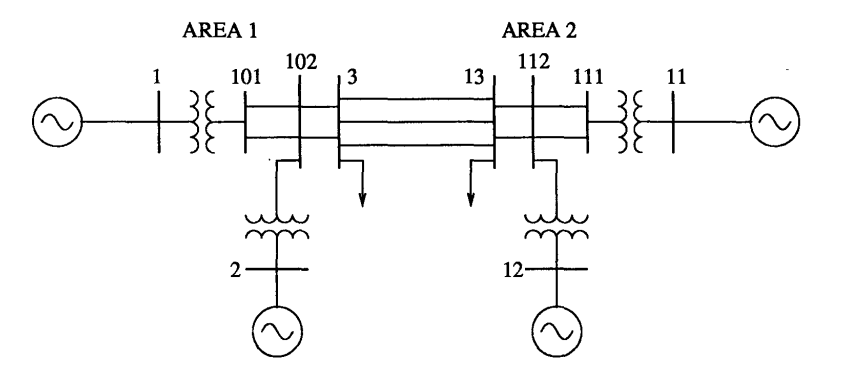
\includegraphics[width=\textwidth]{figures/padiyar_two_area/circuit_diagram.png}
\caption{Padiyar four-machine ten-bus two-area network (source: Padiyar, \emph{Power System Dynamics}, 2nd ed., Sec.~9.6.1) Generators ที่ buses~1 และ~2 อยู่ใน Area~1; generators ที่ buses~11 และ~12 อยู่ใน Area~2 มี 3 parallel circuits เชื่อม buses~3 และ~13 ข้าม inter-area tie โหลดต่ออยู่ที่ buses~3 และ~13}
\end{figure}

\section{Source Data (Padiyar Tables 9.1--9.6)}

ตารางต่อไปนี้คัดลอก verbatim จาก Padiyar, \emph{Power System Dynamics: Stability and Control}, 2nd ed., Section~9.6.1 (printed pages~325--331) ตารางเหล่านี้คือ \emph{input} สำหรับ in-house computation ไม่ใช่ computed result ปริมาณทั้งหมดอยู่บน 100-MVA base

\begin{table}[H]\centering\scriptsize
\caption{Transmission line data บน 100-MVA base (Padiyar Table~9.1)}
\begin{tabular}{ccccc}\toprule
From & To & $R_s$ (pu) & $X_s$ (pu) & $B$ (pu)\\\midrule
1 & 101 & 0.001 & 0.012 & 0.00\\
2 & 102 & 0.001 & 0.012 & 0.00\\
3 & 13  & 0.022 & 0.220 & 0.33\\
3 & 13  & 0.022 & 0.220 & 0.33\\
3 & 13  & 0.022 & 0.220 & 0.33\\
3 & 102 & 0.002 & 0.020 & 0.03\\
3 & 102 & 0.002 & 0.020 & 0.03\\
11 & 111 & 0.001 & 0.012 & 0.00\\
12 & 112 & 0.001 & 0.012 & 0.00\\
13 & 112 & 0.002 & 0.020 & 0.03\\
13 & 112 & 0.002 & 0.020 & 0.03\\
101 & 102 & 0.005 & 0.050 & 0.075\\
101 & 102 & 0.005 & 0.050 & 0.075\\
111 & 112 & 0.005 & 0.050 & 0.075\\
111 & 112 & 0.005 & 0.050 & 0.075\\\bottomrule
\end{tabular}\end{table}

\begin{table}[H]\centering\scriptsize
\caption{Load-flow data และ results --- printed operating point (Padiyar Table~9.2)}
\begin{tabular}{cccccccc}\toprule
Bus & $|V|$ (pu) & $\theta$ (deg) & $P_G$ (pu) & $Q_G$ (pu) & $P_L$ (pu) & $Q_L$ (pu) & $B_{sh}$ (pu)\\\midrule
1   & 1.0300 & 8.2154   & 7.0     & 1.3386 & 0      & 0     & 0\\
2   & 1.0100 & -1.5040  & 7.0     & 1.5920 & 0      & 0     & 0\\
11  & 1.0300 & 0.0      & 7.2172  & 1.4466 & 0      & 0     & 0\\
12  & 1.0100 & -10.2051 & 7.0     & 1.8083 & 0      & 0     & 0\\
101 & 1.0108 & 3.6615   & 0       & 0      & 0      & 0     & 0\\
102 & 0.9875 & -6.2433  & 0       & 0      & 0      & 0     & 0\\
111 & 1.0095 & -4.6977  & 0       & 0      & 0      & 0     & 0\\
112 & 0.9850 & -14.9443 & 0       & 0      & 0      & 0     & 0\\
3   & 0.9761 & -14.4194 & 0       & 0      & 11.59  & 2.12  & 3.0\\
13  & 0.9716 & -23.2922 & 0       & 0      & 15.75  & 2.88  & 4.0\\\bottomrule
\end{tabular}\end{table}

\begin{table}[H]\centering\scriptsize
\caption{Machine data, เหมือนกันทั้งสี่เครื่องเว้นแต่ระบุ (Padiyar Table~9.3)}
\begin{tabular}{lcccc}\toprule
Variable & Bus 1 & Bus 2 & Bus 11 & Bus 12\\\midrule
$X_l$ (pu)        & 0.022   & 0.022   & 0.022   & 0.022\\
$R_a$ (pu)        & 0.00028 & 0.00028 & 0.00028 & 0.00028\\
$X_d$ (pu)        & 0.2     & 0.2     & 0.2     & 0.2\\
$X'_d$ (pu)       & 0.033   & 0.033   & 0.033   & 0.033\\
$T'_{d0}$ (s)     & 8.0     & 8.0     & 8.0     & 8.0\\
$X_q$ (pu)        & 0.19    & 0.19    & 0.19    & 0.19\\
$X'_q$ (pu)       & 0.061   & 0.061   & 0.061   & 0.061\\
$T'_{q0}$ (s)     & 0.4     & 0.4     & 0.4     & 0.4\\
$H$ (s)           & 54.0    & 54.0    & 63.0    & 63.0\\
$D$ (pu)          & 0       & 0       & 0       & 0\\\bottomrule
\end{tabular}\end{table}

\begin{table}[H]\centering
\caption{Excitation system data, single-time-constant AVR (Padiyar Table~9.4)}
\begin{tabular}{lcccc}\toprule
Variable & Bus 1 & Bus 2 & Bus 11 & Bus 12\\\midrule
$K_A$ (pu)  & 200  & 200  & 200  & 200\\
$T_A$ (s)   & 0.02 & 0.02 & 0.02 & 0.02\\\bottomrule
\end{tabular}\end{table}


\begin{table}[H]\centering\scriptsize
\caption{Participation factors ของ swing modes (Padiyar Table~9.6) ($\omega_1=7.29$, $\omega_2=6.69$, $\omega_3=4.44$ rad/s)}
\begin{tabular}{cccc}\toprule
Variable & Mode \#1 & Mode \#2 & Mode \#3\\\midrule
$\Delta S_{m1}$ (bus 1)  & $-0.18 \pm j0.14$  & $0.004 \pm j0.001$ & $-0.06 \pm j0.15$\\
$\Delta S_{m2}$ (bus 2)  & $-0.27 \pm j0.14$  & $0.00 \pm j0.00$   & $-0.062 \pm j0.07$\\
$\Delta S_{m3}$ (bus 11) & $-0.00 \pm j0.00$  & $0.24 \pm j0.03$   & $-0.068 \pm j0.13$\\
$\Delta S_{m4}$ (bus 12) & $-0.04 \pm j0.00$  & $0.30 \pm j0.08$   & $-0.061 \pm j0.07$\\\bottomrule
\end{tabular}\end{table}

Inter-area mode (mode~3, $\omega\approx4.44$~rad/s) มี participation จากทั้งสี่ machines ใกล้เคียงกัน ยืนยันลักษณะ inter-area ของมัน ส่วน Modes~1 และ~2 เป็น local mode ของ Area~1 และ Area~2 ตามลำดับ


\section{การวิเคราะห์ Power Flow}

In-house Newton--Raphson solver ใช้ bus~11 เป็น reference bus ให้ตรงกับมุมศูนย์ที่พิมพ์ใน Table~9.2 Buses 1, 2 และ 12 เป็น PV buses ค่า line susceptance $B$ จาก Table~9.1 ถูกแทนเป็น $B/2$ ที่แต่ละปลายของ standard $\pi$ model ซึ่งเป็น convention ที่ทำให้ reproduce printed operating point ได้

\subsection{Newton--Raphson Formulation}

Solver วนซ้ำบน polar voltage state $x=[\theta_2,\ldots,\theta_N,\, |V|_{PQ_1},\ldots]^T$ (slack angle fixed, PV magnitudes fixed) ค่า bus power injections คำนวณจาก admittance matrix $Y=G+jB$:
\begin{align}
P_i(x) &= |V_i|\sum_{j=1}^{N}|V_j|\bigl(G_{ij}\cos\theta_{ij}+B_{ij}\sin\theta_{ij}\bigr),\\
Q_i(x) &= |V_i|\sum_{j=1}^{N}|V_j|\bigl(G_{ij}\sin\theta_{ij}-B_{ij}\cos\theta_{ij}\bigr),
\end{align}
โดย $\theta_{ij}=\theta_i-\theta_j$ ค่า power mismatch คือ $\Delta P_i=P_i^{\text{spec}}-P_i(x)$, $\Delta Q_i=Q_i^{\text{spec}}-Q_i(x)$ ในแต่ละ iteration Newton step จะแก้สมการ
\begin{equation}
J(x_k)\,\Delta x = \begin{bmatrix}\Delta P\\ \Delta Q\end{bmatrix},
\qquad x_{k+1}=x_k+\Delta x,
\end{equation}
โดย $J$ คือ standard 4-block Jacobian ที่มี sub-matrices $H=\partial P/\partial\theta$, $N=\partial P/\partial|V|$, $M=\partial Q/\partial\theta$, $L=\partial Q/\partial|V|$ การวนซ้ำหยุดเมื่อ $\max|\Delta P,\Delta Q|<10^{-10}$ ไม่มีการใช้ external nonlinear solver; Jacobian สร้างแบบ analytic จาก $Y$ ใน project code


\begin{table}[H]\centering
\caption{Power-flow convergence และ Table~9.2 comparison}
\begin{tabular}{@{}lr@{}}\toprule Quantity & Value\\ \midrule
Converged & Yes\\
Iterations & 3\\
Maximum $|\Delta V|$ vs Table 9.2 & 4.927e-05 pu\\
Maximum $|\Delta \theta|$ vs Table 9.2 & 4.983e-05 deg\\
Total generation & 2821.72 MW\\
Total load & 2734.00 MW\\
Total loss & 87.72 MW\\
\bottomrule\end{tabular}

\end{table}

\begin{table}[H]\centering\small
\caption{Power-flow comparison: Padiyar Table~9.2 เทียบกับ in-house solution ค่า absolute difference ถูกรายงานเพราะ angle แบบเปอร์เซ็นต์ไม่ได้นิยามที่ zero-angle reference bus}
\resizebox{\textwidth}{!}{\begin{tabular}{rrrrrrr}\toprule
{Bus} & {$V_{book}$} & {$V_{ours}$} & {$|\Delta V|$} & {$\theta_{book}$} & {$\theta_{ours}$} & {$|\Delta\theta|$}\\
{} & {(pu)} & {(pu)} & {(pu)} & {(deg)} & {(deg)} & {(deg)}\\ \midrule
1 & 1.0300 & 1.0300 & 0.00e+00 & 8.2154 & 8.2154 & 4.98e-05\\
2 & 1.0100 & 1.0100 & 0.00e+00 & -1.5040 & -1.5040 & 1.13e-05\\
11 & 1.0300 & 1.0300 & 0.00e+00 & 0.0000 & 0.0000 & 0.00e+00\\
12 & 1.0100 & 1.0100 & 0.00e+00 & -10.2051 & -10.2051 & 6.79e-06\\
101 & 1.0108 & 1.0108 & 5.72e-07 & 3.6615 & 3.6615 & 1.83e-05\\
102 & 0.9875 & 0.9875 & 3.06e-05 & -6.2433 & -6.2433 & 2.33e-05\\
111 & 1.0095 & 1.0095 & 3.02e-05 & -4.6977 & -4.6977 & 3.44e-05\\
112 & 0.9850 & 0.9850 & 4.83e-05 & -14.9443 & -14.9443 & 4.15e-05\\
3 & 0.9761 & 0.9761 & 1.43e-05 & -14.4194 & -14.4194 & 3.67e-05\\
13 & 0.9716 & 0.9716 & 4.93e-05 & -23.2922 & -23.2922 & 1.74e-05\\
\bottomrule\end{tabular}
}
\end{table}

\begin{table}[H]\centering\small
\caption{Detailed in-house power-flow results (mirrors launcher output) กำลังทั้งหมดอยู่ใน pu บน 100-MVA base}
\resizebox{\textwidth}{!}{\begin{tabular}{rlrrrrrrrr}\toprule
{Bus} & {Type} & {$|V|$} & {$\theta$} & {$P_G$} & {$Q_G$} & {$P_L$} & {$Q_L$} & {$P_{net}$} & {$Q_{net}$}\\
{} & {} & {(pu)} & {(deg)} & {(pu)} & {(pu)} & {(pu)} & {(pu)} & {(pu)} & {(pu)}\\ \midrule
1 & PV & 1.0300 & 8.2154 & 7.0000 & 1.3386 & 0.0000 & 0.0000 & 7.0000 & 1.3386\\
2 & PV & 1.0100 & -1.5040 & 7.0000 & 1.5920 & 0.0000 & 0.0000 & 7.0000 & 1.5920\\
11 & REF & 1.0300 & 0.0000 & 7.2172 & 1.4466 & 0.0000 & 0.0000 & 7.2172 & 1.4466\\
12 & PV & 1.0100 & -10.2051 & 7.0000 & 1.8083 & 0.0000 & 0.0000 & 7.0000 & 1.8083\\
101 & PQ & 1.0108 & 3.6615 & 0.0000 & 0.0000 & 0.0000 & 0.0000 & 0.0000 & 0.0000\\
102 & PQ & 0.9875 & -6.2433 & 0.0000 & 0.0000 & 0.0000 & 0.0000 & 0.0000 & 0.0000\\
111 & PQ & 1.0095 & -4.6977 & 0.0000 & 0.0000 & 0.0000 & 0.0000 & 0.0000 & 0.0000\\
112 & PQ & 0.9850 & -14.9443 & 0.0000 & 0.0000 & 0.0000 & 0.0000 & 0.0000 & 0.0000\\
3 & PQ & 0.9761 & -14.4194 & 0.0000 & 0.0000 & 11.5900 & 2.1200 & -11.5900 & -2.1200\\
13 & PQ & 0.9716 & -23.2922 & 0.0000 & 0.0000 & 15.7500 & 2.8800 & -15.7500 & -2.8800\\
\bottomrule\end{tabular}
}
\end{table}

\begin{figure}[H]\centering
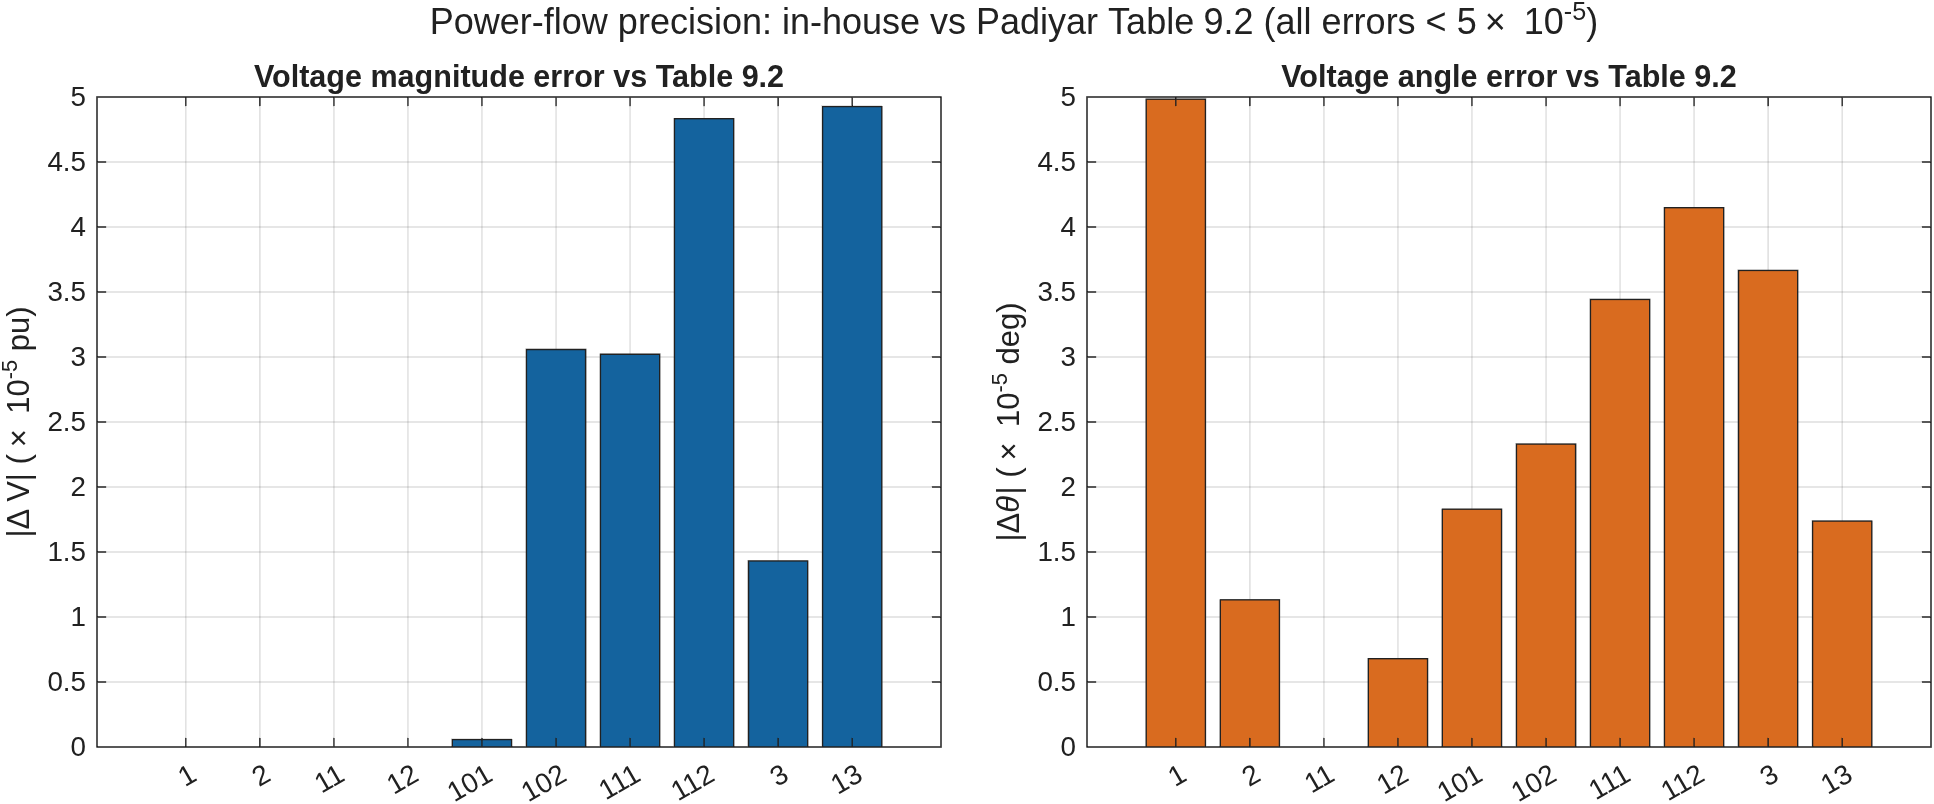
\includegraphics[width=\textwidth]{figures/padiyar_two_area/pf_precision.png}
\caption{Power-flow precision: in-house values เทียบกับ Padiyar Table~9.2 แถวบน---voltage magnitude และ angle scatter พร้อมเส้น 1:1 diagonal (จุดบนเส้นบ่งชี้ exact agreement) แถวล่าง---per-bus absolute errors $|\Delta V|$ และ $|\Delta\theta|$ ทั้งหมดต่ำกว่า $5\times10^{-5}$}
\end{figure}

\begin{figure}[H]\centering

\includegraphics[width=\textwidth]{figures/padiyar_two_area/powerflow_summary.png}
\caption{In-house power-flow result และ Newton--Raphson convergence}
\end{figure}

\section{Model 1.1 ร่วมกับ AVR}

สำหรับ generator $i$ ลำดับ state และ derivative order ที่สอดคล้องกันคือ
\begin{equation}
x_i=\bigl[\delta_i,\ \omega_i,\ E'_{qi},\ E'_{di},\ E_{fdi}\bigr]^T,
\qquad
\dot{x}_i=\bigl[\dot\delta_i,\ \dot\omega_i,\
\dot E'_{qi},\ \dot E'_{di},\ \dot E_{fdi}\bigr]^T
=f_i(x_i,I_{di},I_{qi},|V_i|,u_i),
\end{equation}
โดย dot หมายถึง time derivative ระบบ DAE แบบ input-driven ที่สมบูรณ์คือ
\begin{equation}
\dot x=f(x,y,u),\qquad 0=g(x,y,u),
\label{eq:input-dae}
\end{equation}
โดย
\begin{equation}
\begin{aligned}
y&=\begin{bmatrix}\Re(V)^T&\Im(V)^T\end{bmatrix}^{T},\qquad
u=\begin{bmatrix}P_m^T&u_{exc}^{T}&\rho\end{bmatrix}^{T},\\
u_{exc}&=
\begin{cases}V_{ref},&\text{AVR},\\E_{fd0},&\text{manual excitation}
\end{cases}
\end{aligned}
\label{eq:xyu-order}
\end{equation}
ดังนั้น $x$ คือ differential machine/AVR states, $y$ คือ algebraic bus voltages, และ $u$ คือ prescribed inputs: mechanical power $P_m$, excitation command $u_{exc}$, และ topology selector $\rho$ ใน Equilibrium และ SSSA จะ fixing $u=u_0$ ไว้; ส่วน TS จะเปลี่ยนเฉพาะ $\rho(t)$ ณ declared event times กระแส generator มีเครื่องหมายบวกจาก machine เข้า network สมการ dynamic ที่ implement ใน shared DAE คือ
\begin{align}
\dot\delta_i &= \omega_B(\omega_i-1),\\
2H_i\dot\omega_i &= P_{mi}-P_{ei}-D_i(\omega_i-1),\\
T'_{d0i}\dot E'_{qi} &= E_{fdi}-E'_{qi}-(X_{di}-X'_{di})I_{di},\\
T'_{q0i}\dot E'_{di} &= -E'_{di}+(X_{qi}-X'_{qi})I_{qi},\\
T_{Ai}\dot E_{fdi} &= K_{Ai}(V_{ref,i}-|V_i|)-E_{fdi}.
\end{align}
Transient-saliency stator interface คือ
\begin{align}
V_{di}&=E'_{di}-R_aI_{di}+X'_qI_{qi},\\
V_{qi}&=E'_{qi}-R_aI_{qi}-X'_dI_{di}.
\end{align}
Air-gap electrical power คำนวณโดยตรงเป็น
\begin{equation}
P_{ei}=V_{di}I_{di}+V_{qi}I_{qi}+R_a(I_{di}^2+I_{qi}^2).
\end{equation}
ใช้ nonlinear functions ชุดเดียวกันสำหรับ equilibrium, SSSA และ TS

\subsection{AVR เทียบกับ Manual Excitation}

มีการศึกษา excitation 2 แบบจาก DAE เดียวกัน:
\begin{itemize}
  \item \textbf{With AVR (5 states/machine, 20 total).} Field voltage $E_{fd}$ เป็น dynamic state ที่ควบคุมด้วย single-time-constant AVR ของ Table~9.4 ($K_A=200$, $T_A=0.02$~s):
  \begin{equation}
  T_A\dot E_{fd}=K_A(V_{ref}-|V|)-E_{fd}.
  \label{eq:avr-time}
  \end{equation}
  ที่ equilibrium, $\dot E_{fd}=0$ ดังนั้น voltage error ไม่ได้เป็นศูนย์ แต่เป็น field voltage หารด้วย gain พอดี:
  \begin{equation}
  E_{fd0}=K_A(V_{ref}-|V_0|),\qquad
  V_{ref}=|V_0|+\frac{E_{fd0}}{K_A}.
  \label{eq:avr-equilibrium}
  \end{equation}
  Linearise \eqref{eq:avr-time} ด้วย $\Delta V_{ref}=0$ จะได้
  \begin{equation}
  \Delta E_{fd}(s)=-\frac{K_A}{1+sT_A}\Delta|V|(s).
  \label{eq:avr-transfer}
  \end{equation}
  ดังนั้น $\Delta|V|<0$ ทำให้ $\Delta E_{fd}>0$ DC correction gain คือ 200 และ AVR pole คือ $-1/T_A=-50~\mathrm{s}^{-1}$ ซึ่งอธิบาย fast voltage-support action ทางคณิตศาสตร์ นี่คือ \emph{configuration ที่ตีพิมพ์ในหนังสือ}: Table~9.5 มี 20 eigenvalues พอดี ตรงกับ state count $4\times5=20$ อย่างไรก็ตาม inter-area swing mode มี damping เบามาก สำหรับ $\lambda=\sigma+j\omega_d$,
  \begin{equation}
  \zeta=-\frac{\sigma}{\sqrt{\sigma^2+\omega_d^2}}.
  \label{eq:damping-ratio}
  \end{equation}
  Computed AVR pole $-0.0042+j4.4565$ จึงให้
  \begin{equation}
  \zeta_{AVR}=\frac{0.0042}{\sqrt{0.0042^2+4.4565^2}}
  =9.5\times10^{-4}=0.095\%.
  \end{equation}
  ข้อสรุป lightly damped จึงมาจาก computed pole โดยตรง
  \item \textbf{Manual excitation / no AVR (4 states/machine, 16 total).} การเอา AVR ออกไม่ได้เอา generator field circuit ออก แต่ operator-supplied field voltage จะถูก freeze ไว้ที่ equilibrium value:
  \begin{equation}
  E_{fd}(t)=E_{fd0},\qquad \Delta E_{fd}(s)=0.
  \label{eq:manual-field}
  \end{equation}
  ดังนั้น manual state และ input orders คือ
  \begin{equation}
  x_i^{manual}=
  \begin{bmatrix}\delta_i&\omega_i&E'_{qi}&E'_{di}\end{bmatrix}^{T},
  \qquad
  u_i^{manual}=
  \begin{bmatrix}P_{mi}&E_{fd0,i}&\rho\end{bmatrix}^{T}.
  \label{eq:manual-state-input}
  \end{equation}
  สี่ differential equations ที่คงไว้คือ
  \begin{align}
  \dot\delta_i&=\omega_B(\omega_i-1),\\
  \dot\omega_i&=
  \frac{P_{mi}-P_{ei}-D_i(\omega_i-1)}{2H_i},\\
  \dot E'_{qi}&=
  \frac{E_{fd0,i}-E'_{qi}-(X_{di}-X'_{di})I_{di}}{T'_{d0i}},\\
  \dot E'_{di}&=
  \frac{-E'_{di}+(X_{qi}-X'_{qi})I_{qi}}{T'_{q0i}}.
  \label{eq:manual-dynamics}
  \end{align}
  ดังนั้น manual excitation ยังคงมี rotor, speed, $d$-axis flux, $q$-axis flux, stator-current และ network-voltage dynamics สิ่งที่หายไปคือ closed-loop field-voltage state และ terminal-voltage feedback เท่านั้น

  Linearise สมการที่สามใน \eqref{eq:manual-dynamics} จะได้
  \begin{equation}
  \Delta\dot E'_q=
  -\frac{1}{T'_{d0}}\Delta E'_q
  -\frac{X_d-X'_d}{T'_{d0}}\Delta I_d
  +\frac{1}{T'_{d0}}\underbrace{\Delta E_{fd}}_{0}.
  \label{eq:manual-linear-field}
  \end{equation}
  เปรียบเทียบกับ AVR perturbation ที่ได้จาก \eqref{eq:avr-time}:
  \begin{equation}
  \Delta\dot E_{fd}
  =-\frac{1}{T_A}\Delta E_{fd}
   -\frac{K_A}{T_A}\Delta|V|
   +\frac{K_A}{T_A}\Delta V_{ref}.
  \label{eq:avr-linear-field}
  \end{equation}
  เมื่อ $\Delta V_{ref}=0$, AVR จะเพิ่ม coupling $-(K_A/T_A)\Delta|V|$ และอีกหนึ่ง state เข้ามา ส่วน manual excitation ไม่มีทั้งสอง term ใน state-matrix form จะได้
  \begin{equation}
  \begin{aligned}
  \Delta\dot x_{manual}&=A_{manual}\Delta x_{manual},
  &A_{manual}&\in\mathbb{R}^{16\times16},\\
  \Delta\dot x_{AVR}&=A_{AVR}\Delta x_{AVR},
  &A_{AVR}&\in\mathbb{R}^{20\times20}.
  \end{aligned}
  \end{equation}
  No-AVR ไม่ได้หมายถึง terminal voltage คงที่: $V$ ยังคงเป็น algebraic solution ของ $g(x,y,u)=0$ และเปลี่ยนแปลงเมื่อ machine current หรือ network topology เปลี่ยน มีเพียง $E_{fd}$ ที่คงที่

  Manual case นี้เป็น 16-state study แยกต่างหาก, ไม่ได้ reproduce 20-state Table~9.5 ค่า computed inter-area pole $-0.1173+j4.0712$ ให้
  \begin{equation}
  \zeta_{manual}=\frac{0.1173}{\sqrt{0.1173^2+4.0712^2}}
  =0.0288=2.88\%.
  \end{equation}
  การเปรียบเทียบจึงอยู่บนพื้นฐาน equation-based: AVR ช่วยเรื่อง voltage regulation ผ่าน \eqref{eq:avr-transfer} ขณะที่เพิ่ม feedback block \eqref{eq:avr-linear-field} ทำให้ full system matrix เปลี่ยนและย้าย inter-area pole จาก $\zeta=2.88\%$ ไปเป็น $\zeta=0.095\%$ ข้อสังเกตนี้ใช้กับ operating point และ printed AVR parameters ที่ระบุเท่านั้น ไม่ใช่ universal claim ว่า AVR ทุกตัวลด damping
\end{itemize}
หนังสือใช้ AVR ตลอด Section~9.6.1: Table~9.4 ให้ AVR parameters และ Table~9.5 รายงาน 20-state eigenvalue spectrum ส่วน manual case เป็น project-defined comparison ไม่ใช่ book configuration

\section{Small-Signal Stability (SSSA)}

DAE ทั้งหมดถูก linearise เชิงตัวเลขรอบ in-house power-flow operating point ส่วน algebraic network-voltage perturbations ถูก eliminate ด้วย Schur complement ค่า published eigenvalues ถูก transcribe ในตารางด้านล่าง (Source data) ไม่ได้ถูก copy ไปยัง computed column และไม่ได้ใช้ tune parameters

\subsection{Linearisation และ Schur Reduction}

Nonlinear DAE ใน \eqref{eq:input-dae} ถูก linearise รอบ $(x_0,y_0,u_0)$ หลังจากตรวจสอบว่า
\begin{equation}
\|f(x_0,y_0,u_0)\|_\infty\le\varepsilon_{eq},\qquad
\|g(x_0,y_0,u_0)\|_\infty\le\varepsilon_{eq}.
\end{equation}
SSSA จะ fixing external input $\Delta u=0$ แทนค่า $x=x_0+\Delta x$ และ $y=y_0+\Delta y$ และเก็บ first-order terms จะได้
\begin{equation}
\begin{bmatrix}\Delta\dot x\\0\end{bmatrix}
=
\begin{bmatrix}J_{xx}&J_{xy}\\J_{yx}&J_{yy}\end{bmatrix}
\begin{bmatrix}\Delta x\\\Delta y\end{bmatrix}.
\label{eq:sssa-linear-dae}
\end{equation}
Jacobian blocks คือ
\begin{equation}
J_{xx}=\tfrac{\partial f}{\partial x},\quad
J_{xy}=\tfrac{\partial f}{\partial y},\quad
J_{yx}=\tfrac{\partial g}{\partial x},\quad
J_{yy}=\tfrac{\partial g}{\partial y}.
\end{equation}
ค่าทั้งหมดประเมินด้วย central differences เช่น
\begin{align}
J_{xx}(:,k)&\approx
\frac{f(x_0+h e_k,y_0,u_0)-f(x_0-h e_k,y_0,u_0)}{2h},\\
J_{yx}(:,k)&\approx
\frac{g(x_0+h e_k,y_0,u_0)-g(x_0-h e_k,y_0,u_0)}{2h},
\end{align}
ด้วย $h=10^{-6}$; $J_{xy}$ และ $J_{yy}$ ใช้ $y_0\pm h e_k$ เหล่านี้คือ derivatives ของ DAE equations ไม่ใช่ derivatives ของ reference table

Algebraic row ถูกแก้เป็น
\begin{equation}
J_{yy}\Delta y=-J_{yx}\Delta x.
\end{equation}
Code คำนวณ $K=J_{yy}\backslash J_{yx}$ เพื่อหลีกเลี่ยง explicit inverse และแทน $\Delta y=-K\Delta x$ ลงใน differential row:
\begin{equation}
A=J_{xx}-J_{xy}K
=J_{xx}-J_{xy}J_{yy}^{-1}J_{yx},\qquad
\Delta\dot x=A\Delta x.
\label{eq:sssa-schur}
\end{equation}

\subsection{Eigenvalue Solution และ Modal Quantities}

Solver จากนั้นประเมิน
\begin{equation}
A v_i=\lambda_i v_i,\qquad
\det(\lambda_iI-A)=0,qquad \lambda_i=\sigma_i+j\omega_{d,i}.
\end{equation}
สำหรับแต่ละ conjugate pair
\begin{equation}
f_i=\frac{|\omega_{d,i}|}{2\pi},\qquad
\zeta_i=-\frac{\sigma_i}{\sqrt{\sigma_i^2+\omega_{d,i}^2}},\qquad
\tau_i=-\frac{1}{\sigma_i}\quad(\sigma_i<0).
\label{eq:sssa-modal-metrics}
\end{equation}
Physical mode จะ asymptotically stable เมื่อ $\sigma_i<0$ Table~9 ใช้ full 20-state AVR matrix ตรงกับ original-matrix column ของ Padiyar Table~9.5 ส่วน optional COI reduction ถูก disable อย่างชัดแจ้งในการรันนี้ ดังนั้น rotational reference-angle mode จะอยู่ใกล้ origin และไม่ถูก misclassify เป็น unstable physical mode Table~10 เลือก positive-imaginary roots ด้วย $1<\omega_d<10$ rad/s; conjugates ที่ละไว้มี $f$ และ $\zeta$ เหมือนกัน

Reference matching เกิดขึ้นหลัง \eqref{eq:sssa-schur} ถูกแก้แล้วเท่านั้น การ assign แบบ one-to-one จะ minimize $|\lambda_{ours}-\lambda_{book}|$ โดยไม่เปลี่ยน $A$ หรือ model parameter ค่า reported errors คือ
\begin{equation}
\varepsilon_\lambda=
100\frac{|\lambda_{ours}-\lambda_{book}|}{|\lambda_{book}|},\quad
\varepsilon_f=100\frac{|f_{ours}-f_{book}|}{f_{book}},\quad
\varepsilon_\zeta=
100\frac{|\zeta_{ours}-\zeta_{book}|}{|\zeta_{book}|}.
\end{equation}
Eigenvalue percentage ถูกละไว้สำหรับ near-zero reference pair เพราะ denominator ทำให้ relative error ไม่มีความหมายเชิงตัวเลข

\begin{table}[H]\centering\small
\caption{Eigenvalue comparison: ค่าจากหนังสือ ($\lambda_{book}$, Padiyar Table~9.5) เทียบกับ in-house computed values ($\lambda_{ours}$) พร้อม absolute difference $|\Delta\lambda|$ และ swing-mode labels ค่า percentage error ถูกละไว้สำหรับ near-zero reference-angle modes เพราะไม่มีความหมายเชิงตัวเลข และ 18 non-reference modes ทั้งหมด stable}




\resizebox{\textwidth}{!}{\begin{tabular}{rccrcl}\toprule
{No.} & {$\lambda_{book}$} & {$\lambda_{ours}$} & {$|\Delta\lambda|$} & {$\varepsilon_{\lambda}$} & {Mode}\\
{} & {(s$^{-1}$)} & {(s$^{-1}$)} & {(s$^{-1}$)} & {(\%)} & {}\\ \midrule
1 & $-39.9893$ & $-40.0225$ & 0.0332 & {0.08} & \\
2 & $-39.4922$ & $-39.5270$ & 0.0348 & {0.09} & \\
3 & $-24.5058 +20.6749j$ & $-24.5061 +20.6319j$ & 0.0430 & {0.13} & \\
4 & $-24.5058 -20.6749j$ & $-24.5061 -20.6319j$ & 0.0430 & {0.13} & \\
5 & $-25.0383 +11.9973j$ & $-25.0384 +11.9598j$ & 0.0375 & {0.13} & \\
6 & $-25.0383 -11.9973j$ & $-25.0384 -11.9598j$ & 0.0375 & {0.13} & \\
7 & $-11.5835$ & $-11.5566$ & 0.0269 & {0.23} & \\
8 & $-11.1735$ & $-11.1485$ & 0.0250 & {0.22} & \\
9 & $-0.7594 +7.2938j$ & $-0.7553 +7.3157j$ & 0.0223 & {0.30} & Swing 1\\
10 & $-0.7594 -7.2938j$ & $-0.7553 -7.3157j$ & 0.0223 & {0.30} & Swing 1\\
11 & $-0.7365 +6.6899j$ & $-0.7336 +6.7108j$ & 0.0211 & {0.31} & Swing 2\\
12 & $-0.7365 -6.6899j$ & $-0.7336 -6.7108j$ & 0.0211 & {0.31} & Swing 2\\
13 & $-0.0044 +4.4444j$ & $-0.0042 +4.4565j$ & 0.0121 & {0.27} & Inter-area\\
14 & $-0.0044 -4.4444j$ & $-0.0042 -4.4565j$ & 0.0121 & {0.27} & Inter-area\\
15 & $-4.5727$ & $-4.5701$ & 0.0026 & {0.06} & \\
16 & $-4.4802$ & $-4.4776$ & 0.0026 & {0.06} & \\
17 & $-4.1121$ & $-4.1095$ & 0.0026 & {0.06} & \\
18 & $0.0000 +0.0017j$ & $0.0000 +0.0000j$ & 0.0017 & {--} & \\
19 & $0.0000 -0.0017j$ & $0.0000 -0.0000j$ & 0.0017 & {--} & \\
20 & $-4.2449$ & $-4.2423$ & 0.0026 & {0.06} & \\
\bottomrule\end{tabular}
}
\end{table}

\begin{figure}[H]\centering
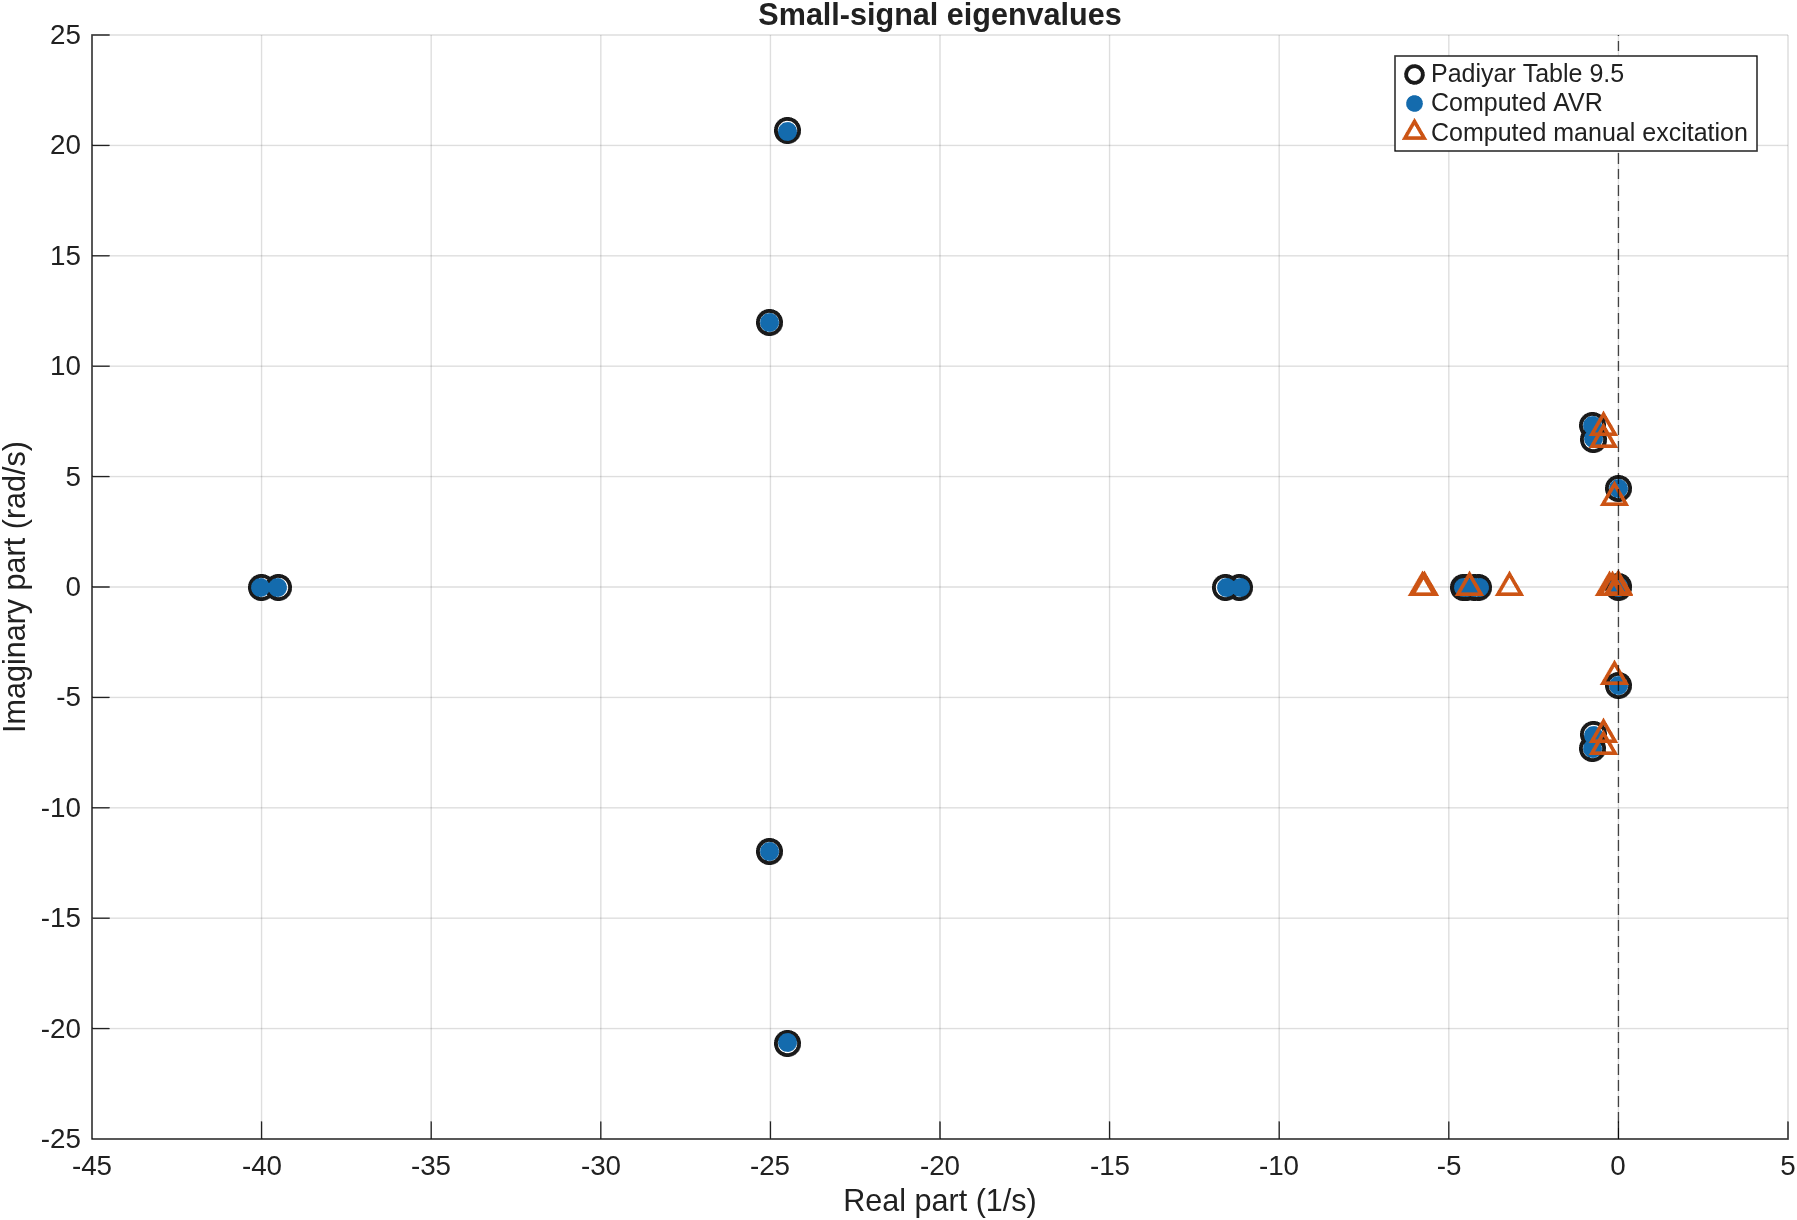
\includegraphics[width=.92\textwidth]{figures/padiyar_two_area/eigenvalue_comparison.png}
\caption{Graphical counterpart ของ Table~9 โดยใช้เพียง AVR comparison บน complex-plane เดียว ค่าที่ transcribe อิสระจาก Padiyar Table~9.5 เป็นวงกลม และ computed AVR eigenvalues เป็นกากบาท เครื่องหมายที่ซ้อนทับกันแสดง direct graphical agreement}
\end{figure}

\begin{table}[H]\centering
\caption{SSSA swing-mode comparison แต่ละแถว AVR เปรียบเทียบโดยตรงระหว่าง published และ in-house eigenvalue, frequency และ damping ratio ส่วน manual excitation ไม่มี published counterpart เพราะมี state count ต่างกัน เซลล์ reference ที่ไม่มีจะแสดงด้วยขีด ทั้ง frequency และ damping-ratio percentage errors คำนวณโดยตรงจากค่าที่แสดง}
\resizebox{\textwidth}{!}{\begin{tabular}{llccrrrrrr}\toprule
{Configuration} & {Mode} & {$\lambda_{book}$} & {$\lambda_{ours}$} & {$f_{book}$} & {$f_{ours}$} & {$\varepsilon_f$} & {$\zeta_{book}$} & {$\zeta_{ours}$} & {$\varepsilon_{\zeta}$}\\
{} & {} & {(s$^{-1}$)} & {(s$^{-1}$)} & {(Hz)} & {(Hz)} & {(\%)} & {(\%)} & {(\%)} & {(\%)}\\ \midrule
AVR & Inter-area & $-0.0044+4.4444j$ & $-0.0042+4.4565j$ & 0.7073 & 0.7093 & 0.27 & 0.099 & 0.095 & 3.79\\
AVR & Local Area 2 & $-0.7365+6.6899j$ & $-0.7336+6.7108j$ & 1.0647 & 1.0680 & 0.31 & 10.943 & 10.867 & 0.70\\
AVR & Local Area 1 & $-0.7594+7.2938j$ & $-0.7553+7.3157j$ & 1.1608 & 1.1643 & 0.30 & 10.356 & 10.269 & 0.83\\
Manual & Inter-area & {--} & $-0.1173+4.0712j$ & {--} & 0.6480 & {--} & {--} & 2.880 & {--}\\
Manual & Local Area 2 & {--} & $-0.4296+6.6775j$ & {--} & 1.0627 & {--} & {--} & 6.420 & {--}\\
Manual & Local Area 1 & {--} & $-0.4460+7.2336j$ & {--} & 1.1513 & {--} & {--} & 6.154 & {--}\\
\bottomrule\end{tabular}
}
\end{table}

\begin{figure}[H]\centering
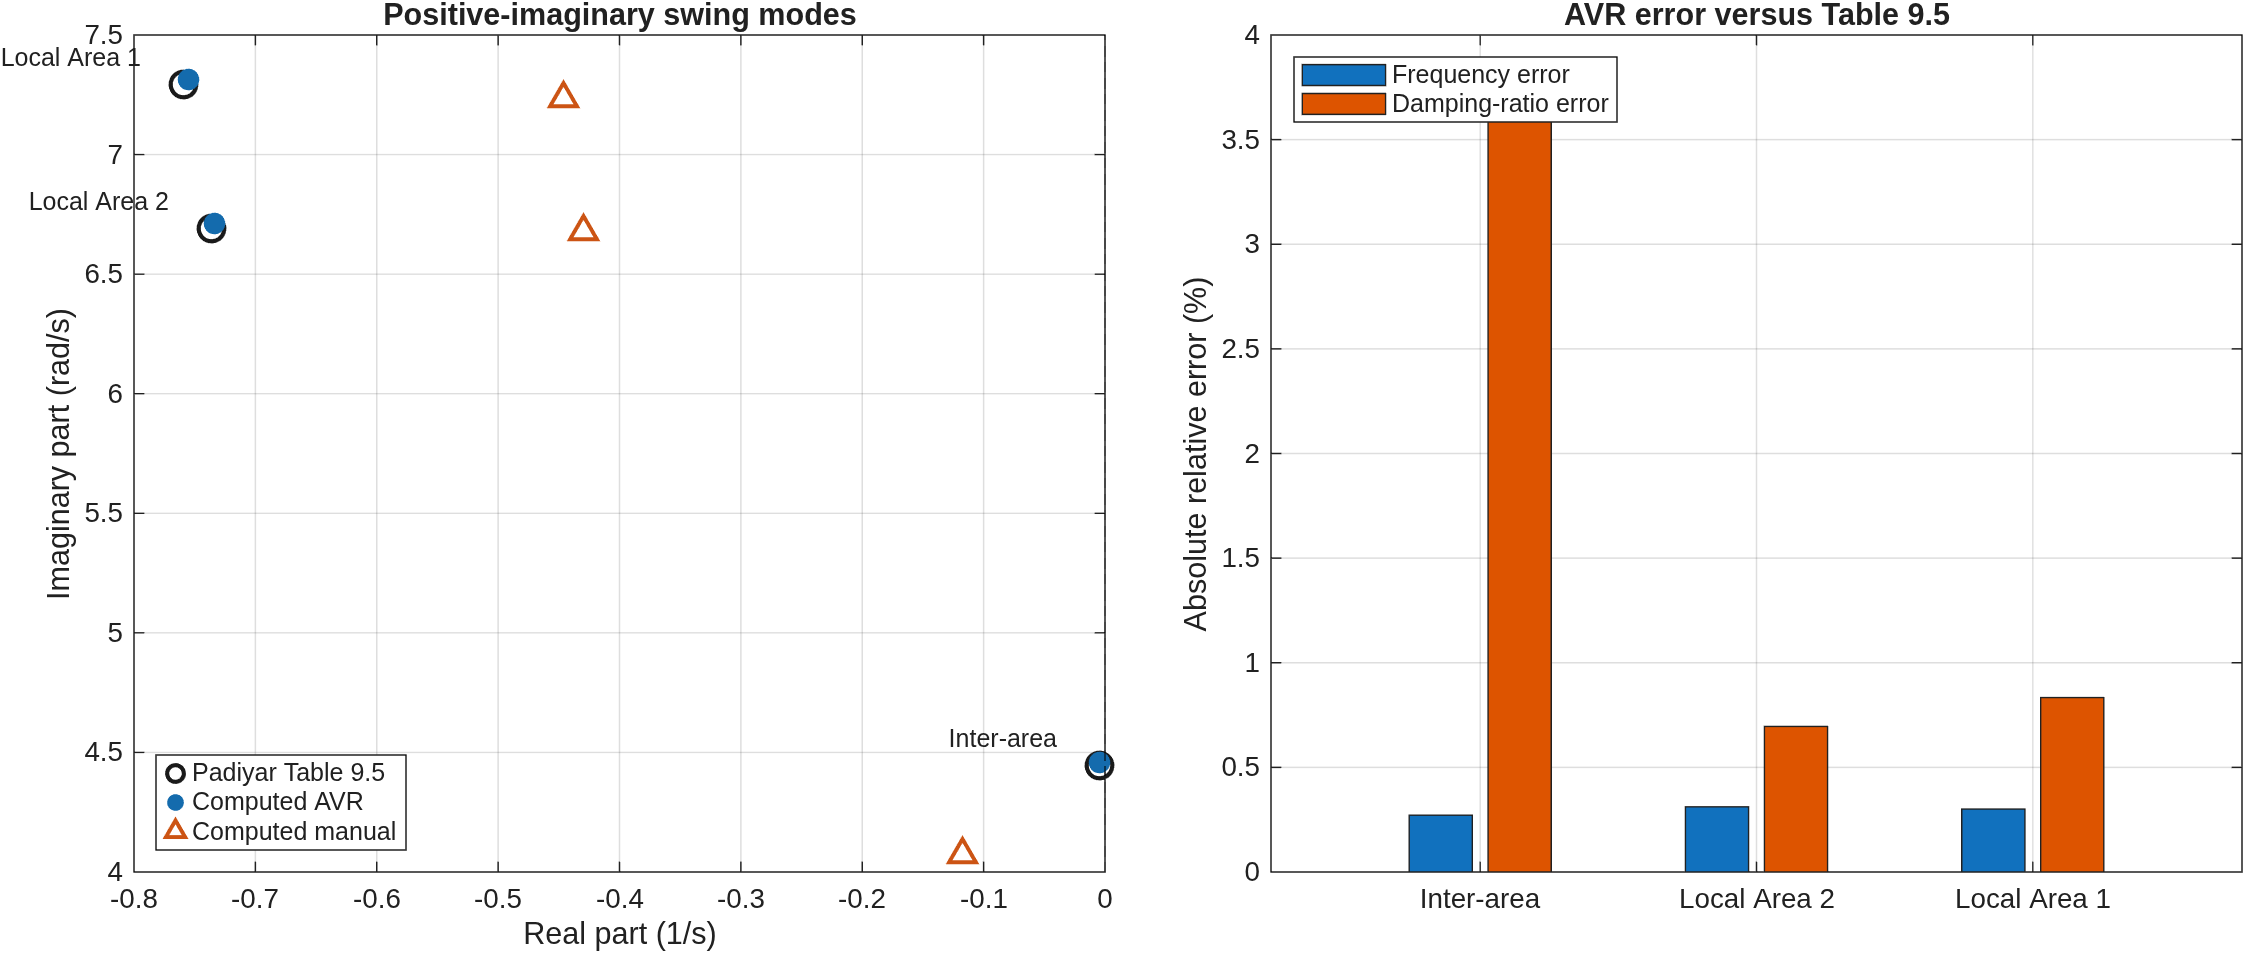
\includegraphics[width=\textwidth]{figures/padiyar_two_area/swing_mode_comparison.png}
\caption{Graphical counterpart ของ Table~10 ซ้าย: positive-imaginary swing-mode eigenvalues ขวา: AVR frequency และ damping-ratio errors เทียบกับ published values ส่วน manual case ถูก plot เฉพาะใน complex plane เพราะไม่มี published manual-excitation target}
\end{figure}


AVR case ทำซ้ำ published mode groups ได้โดยไม่ copy table ความแตกต่างถูกรายงานเป็น model/numerical discrepancies แทนที่จะถูกลบออกด้วยการ calibrate ส่วน manual excitation เป็น 16-state study แยกต่างหาก และไม่ได้คาดหวังให้ reproduce 20-state AVR table

\section{Time-Domain Simulation (TDS)}

Source pages ไม่ได้ระบุ time-domain fault scenario สำหรับ controlled comparison รายงานฉบับนี้กำหนด project scenario: temporary balanced fault ที่ bus~101, $Z_f=j(10\times10^{-5})=j10^{-4}$ pu ใช้ที่ 1.0~s และ clear ที่ 1.1~s จำลองจาก 0 ถึง 20.0~s ด้วย $\Delta t=0.005$~s โครงข่าย จุดทำงาน และ disturbance ชุดเดียวกันถูกใช้สำหรับ manual และ AVR configurations วิธีนี้ใช้ fixed nominal time step, exact event samples และ iterative implicit-trapezoidal corrector

\subsection{Implicit Trapezoidal Integration}

\subsubsection{ทำไมจึงใช้ Implicit Trapezoidal Method}

การเลือกนี้เป็นเชิง numerical ไม่ใช่ post-result fit ให้ได้ trajectory ที่ต้องการ โมเดล Padiyar ที่ implement เป็น semi-explicit DAE system
\begin{equation}
 \dot{x}=f(x,y,u),\qquad 0=g(x,y,Y),
 \label{eq:ts-dae-interface}
\end{equation}
โดย machine states $x$ evolve พร้อมกับ algebraic network voltages $y$ การใช้ trapezoidal quadrature กับ differential equation ในช่วงหนึ่งที่มีความยาว $h$ ให้
\begin{equation}
 x_{n+1}=x_n+\frac{h}{2}\left[f(x_n,y_n,u_n)
                  +f(x_{n+1},y_{n+1},u_{n+1})\right],
 \qquad g(x_{n+1},y_{n+1},Y_{n+1})=0.
 \label{eq:ts-trapezoidal-update}
\end{equation}
สมการ~\eqref{eq:ts-trapezoidal-update} คือสมการที่แก้จริงโดย \path{stability.ts_step_kernel}; algebraic endpoint condition ถูกแก้โดย \path{stability.ts_algebraic_solve} เหตุผลต่อไปนี้เป็น project derivation จาก implemented equation นั้น ไม่ใช่ claim ว่า reference พิมพ์ project code ตรงตามตัวอักษร

ประการแรก สำหรับ smooth exact solution, Taylor expansion รอบ $t_n$ ให้ one-step defect
\begin{equation}
x(t_n+h)-x(t_n)-\frac{h}{2}\left[\dot{x}(t_n)+\dot{x}(t_n+h)\right]
=-\frac{h^3}{12}x^{(3)}(t_n)+\mathcal{O}(h^4).
\label{eq:ts-trapezoidal-order}
\end{equation}
ดังนั้น trapezoidal quadrature มี one-step truncation error $\mathcal{O}(h^3)$ และ global order 2 จึงช่วยปรับปรุง time-discretisation accuracy เหนือ first-order backward Euler ที่ nominal step เดียวกัน พร้อมยังคง implicit endpoint solve ประการที่สอง linear stability สามารถดูได้โดยไม่ต้องพึ่ง plot สำหรับ test equation $\dot{x}=\lambda x$ ด้วย $z=h\lambda$ จะได้
\begin{equation}
 x_{n+1}=R(z)x_n,\qquad
 R(z)=\frac{1+z/2}{1-z/2}.
 \label{eq:ts-trapezoidal-stability}
\end{equation}
ถ้า $\operatorname{Re}(z)\le0$ แล้ว $|1-z/2|^2-|1+z/2|^2=-2\operatorname{Re}(z)\ge0$ ดังนั้น $|R(z)|\le1$ วิธีนี้จึงเป็น A-stable: stable continuous modes จะไม่ถูกทำให้ unstable เพียงเพราะ stability region ของ explicit method เล็กเกินไป ประเด็นนี้มีประโยชน์สำหรับ coupled machine--network DAE ซึ่ง electrical และ electromechanical modes อาจมี time scales ต่างกันมาก อย่างไรก็ตาม step size ยังคงเลือกเพื่อ accuracy และ event resolution ไม่ได้ทำให้ใหญ่โดยพลการเพียงเพราะ method เป็น A-stable

ประการที่สาม implicit endpoint formulation อนุญาตให้ network constraint $g=0$ ถูก re-solve ที่แต่ละ accepted endpoint เมื่อ fault ถูก apply หรือ clear, integration grid จะลงจอดตรง declared event time พอดี, network topology ถูก switch และ algebraic voltage ถูก re-solve ภายใต้ new topology ดังนั้น stored event sample จึง consistent กับ DAE แทนที่จะได้มาจากการ interpolate ข้าม discontinuous network change

วิธีนี้ก็มีข้อจำกัดเช่นกัน: มันไม่เป็น L-stable เพราะ $R(z)\rightarrow-1$ เมื่อ $z\rightarrow-\infty$; very fast decaying components จะไม่ถูก annihilate ในหนึ่ง large step และอาจปรากฏเป็น numerical ringing ถ้า $h$ ถูกเลือกใหญ่เกินไป ทุก step ยังต้องการ nonlinear corrector และ algebraic Newton iterations ด้วย Implementation จึงตรวจสอบทั้ง trapezoidal residual และ algebraic residual และจะ fail-closed เมื่อ iterations เหล่านั้นไม่ converge การตรวจสอบ accuracy และ convergence เหล่านี้ ไม่ใช่เพียง A-stability อย่างเดียว ที่เป็นเหตุผลให้ accepted TDS result มีความน่าเชื่อถือ

Topology input เป็น piecewise constant:
\begin{equation}
Y(t)=
\begin{cases}
Y_{pre},&t<t_f,\\
Y_{fault},&t_f\le t<t_c,\\
Y_{post},&t\ge t_c,
\end{cases}
\qquad
Y_{fault}=Y_{pre}+\frac{1}{Z_f}e_fe_f^T.
\label{eq:ts-topology}
\end{equation}
โดย $e_f$ เลือก faulted bus เวลา $t_f$ และ $t_c$ ถูก insert ตรงเข้าไปใน nominal $\Delta t$ grid ดังนั้นไม่มี step ใดซ่อน topology transition

ที่แต่ละ accepted state $x$ ค่า network voltage ได้มาจาก
\begin{equation}
g(x,y,Y)=0.
\label{eq:ts-algebraic}
\end{equation}
สำหรับ algebraic Newton iteration $k$ กำหนด $r_g^{(k)}=g(x,y^{(k)},Y)$ และ $G_y^{(k)}=\partial g/\partial y$ จากนั้น
\begin{equation}
G_y^{(k)}\Delta y^{(k)}=-r_g^{(k)},\qquad
y^{(k+1)}=y^{(k)}+\alpha_k\Delta y^{(k)}.
\label{eq:ts-network-newton}
\end{equation}
Line search ลอง $\alpha_k=1,1/2,1/4,\ldots,2^{-16}$ และยอมรับค่าแรกที่ลด $\|r_g\|_\infty$ ลง Algebraic solve ต้องการ $\|r_g\|_\infty\le10^{-11}$ และจะ refresh $G_y$ ด้วย central differences ถ้า step ถูก reject

สำหรับ $h=t_{n+1}-t_n$ และ $f_n=f(x_n,y_n,u_n)$ ค่า predictor คือ
\begin{equation}
\hat x^{(0)}_{n+1}=x_n+h f_n,\qquad
\hat y^{(0)}_{n+1}=y_n.
\label{eq:ts-predictor}
\end{equation}
Corrector iteration $c$ ทำลำดับต่อไปนี้:
\begin{align}
g(\hat x^{(c)}_{n+1},\hat y^{(c)}_{n+1},Y_n)&=0,\\
x^{(c+1)}_{n+1}
 &=x_n+\frac{h}{2}\left[f_n+
 f(\hat x^{(c)}_{n+1},\hat y^{(c)}_{n+1},u_n)\right],\\
g(x^{(c+1)}_{n+1},y^{(c+1)}_{n+1},Y_n)&=0,\\
R^{(c+1)}_{trap}
 &=x^{(c+1)}_{n+1}-x_n-\frac{h}{2}\left[f_n+
 f(x^{(c+1)}_{n+1},y^{(c+1)}_{n+1},u_n)\right].
\label{eq:ts-corrector}
\end{align}
Next iterate ใช้ $\hat x^{(c+1)}_{n+1}=x^{(c+1)}_{n+1}$ การยอมรับต้องผ่านทั้งสองเงื่อนไข
\begin{equation}
\|x^{(c+1)}_{n+1}-\hat x^{(c)}_{n+1}\|_\infty\le\tau_n,
\qquad
\|R^{(c+1)}_{trap}\|_\infty\le\tau_n,
\end{equation}
โดย implemented mixed tolerance คือ
\begin{equation}
\tau_n=10^{-10}+10^{-8}\max\left(1,\|x^{(c+1)}_{n+1}\|_\infty\right).
\end{equation}
อนุญาต corrector iterations สูงสุด 12 ครั้ง หาก failed corrector จะ raise error แทนที่จะยอมรับ step หลังการยอมรับ $Y(t_{n+1})$ จะถูกเลือกอีกครั้งและ \eqref{eq:ts-algebraic} ถูก solve ทำให้มั่นใจว่า stored event sample สอดคล้องกับ new topology

\subsection{Fixed Corrector Iteration เทียบกับ Adaptive Time Stepping}

Corrector iteration และ time-step controller แก้ปัญหาต่างกัน สำหรับ fixed $h$ การทำ correction ซ้ำจะขับเคลื่อน nonlinear equation residual
\begin{equation}
F_h(x_{n+1})=
x_{n+1}-x_n-\frac{h}{2}\left(f_n+f_{n+1}\right)
\end{equation}
ให้เข้าใกล้ศูนย์ ดังนั้น $\|F_h\|_\infty\ll1$ พิสูจน์ว่า trapezoidal equation สำหรับ $h$ ที่เลือกถูกแก้อย่างแม่นยำ แต่ไม่ได้ประเมิน discretization error $\|x(t_{n+1})-x_{n+1}\|$

Adaptive second-order trapezoidal method ยังต้องการ independent local-error estimate แบบหนึ่ง การทำ step doubling จะคำนวณหนึ่ง full step $x_h$ และสอง half steps $x_{h/2,h/2}$ แล้วสร้าง
\begin{equation}
e_n=\frac{x_{h/2,h/2}-x_h}{2^2-1},\qquad
E_n=\left\|
\frac{e_n}{a_{tol}+r_{tol}\max(|x_n|,|x_{h/2,h/2}|)}
\right\|_\infty.
\label{eq:adaptive-estimator}
\end{equation}
Step จะถูกยอมรับเฉพาะเมื่อ $E_n\le1$; มิฉะนั้นจะถูก reject และ recompute ตัวอย่าง controller คือ
\begin{equation}
h_{new}=h\,
\operatorname{clip}\left(f_{min},f_{max},
safety\,E_n^{-1/3}\right),
\label{eq:adaptive-controller}
\end{equation}
โดย event times จะกำหนด upper bound ของ $h_{new}$ เพื่อให้ solver ยังคง landing ตรง $t_f$ และ $t_c$ พอดี

Validation solver ปัจจุบันตั้งใจคงเป็น fixed-step เพราะ published comparison protocol ต้องการ deterministic common output grid และ implementation ปัจจุบันยังไม่มีทั้ง independent estimator \eqref{eq:adaptive-estimator} และ step rejection การเรียก corrector iteration ว่า adaptive จึงไม่ถูกต้อง ค่า fixed $h=0.005$~s ถูกยอมรับที่นี่เฉพาะหลัง equilibrium, residual, convergence และ finite-trajectory checks แล้วเท่านั้น ไม่ได้นำเสนอเป็น general proof ของ time-discretization accuracy ส่วน adaptive stepping เป็น valid future production improvement แต่ต้องเพิ่ม estimator, accept/reject controller, exact event landing, resampling สำหรับ cross-tool comparison และ convergence tests ภายใต้ tighter tolerances ก่อนที่จะแทนที่ reproducible validation path นี้

Recorded outputs ถูก reconstruct จาก accepted $(x_n,y_n)$:
\begin{equation}
|V_b|=\sqrt{y_{2b-1}^2+y_{2b}^2},\qquad
P_{ei}=V_{di}I_{di}+V_{qi}I_{qi}+R_a(I_{di}^2+I_{qi}^2),
\end{equation}
ด้วย $P_{ei}[\mathrm{MW}]=S_{base}[\mathrm{MVA}]P_{ei}[\mathrm{pu}]$ ส่วน saved diagnostics ประกอบด้วย initial DAE residual, corrector update norm, trapezoidal residual, iteration count, convergence flag และ non-converged-step count; ดังนั้น plausible plot จะไม่สามารถซ่อน failed numerical step ได้

\begin{table}[H]\centering
\caption{Time-domain simulation input contract, numerical status และ response extrema สำหรับ 0--20~s bus-101 fault scenario ด้วย $Z_f=j10^{-4}$~pu, $t_f=1.0$~s, $t_c=1.1$~s และ $\Delta t=0.005$~s}
\label{tab:ts-summary}
\begin{tabular}{llrr}\toprule {Metric} & {Unit} & {AVR} & {Manual excitation}\\ \midrule
Initial DAE residual & pu & 9.215e-13 & 5.684e-14\\
Non-converged steps & steps & 0 & 0\\
Maximum corrector residual & pu & 7.676e-09 & 5.107e-10\\
Minimum bus voltage & pu & 0.9244 & 0.9184\\
Maximum speed deviation & pu & 4.397e-04 & 8.002e-04\\
\bottomrule\end{tabular}

\end{table}

\begin{figure}[H]\centering
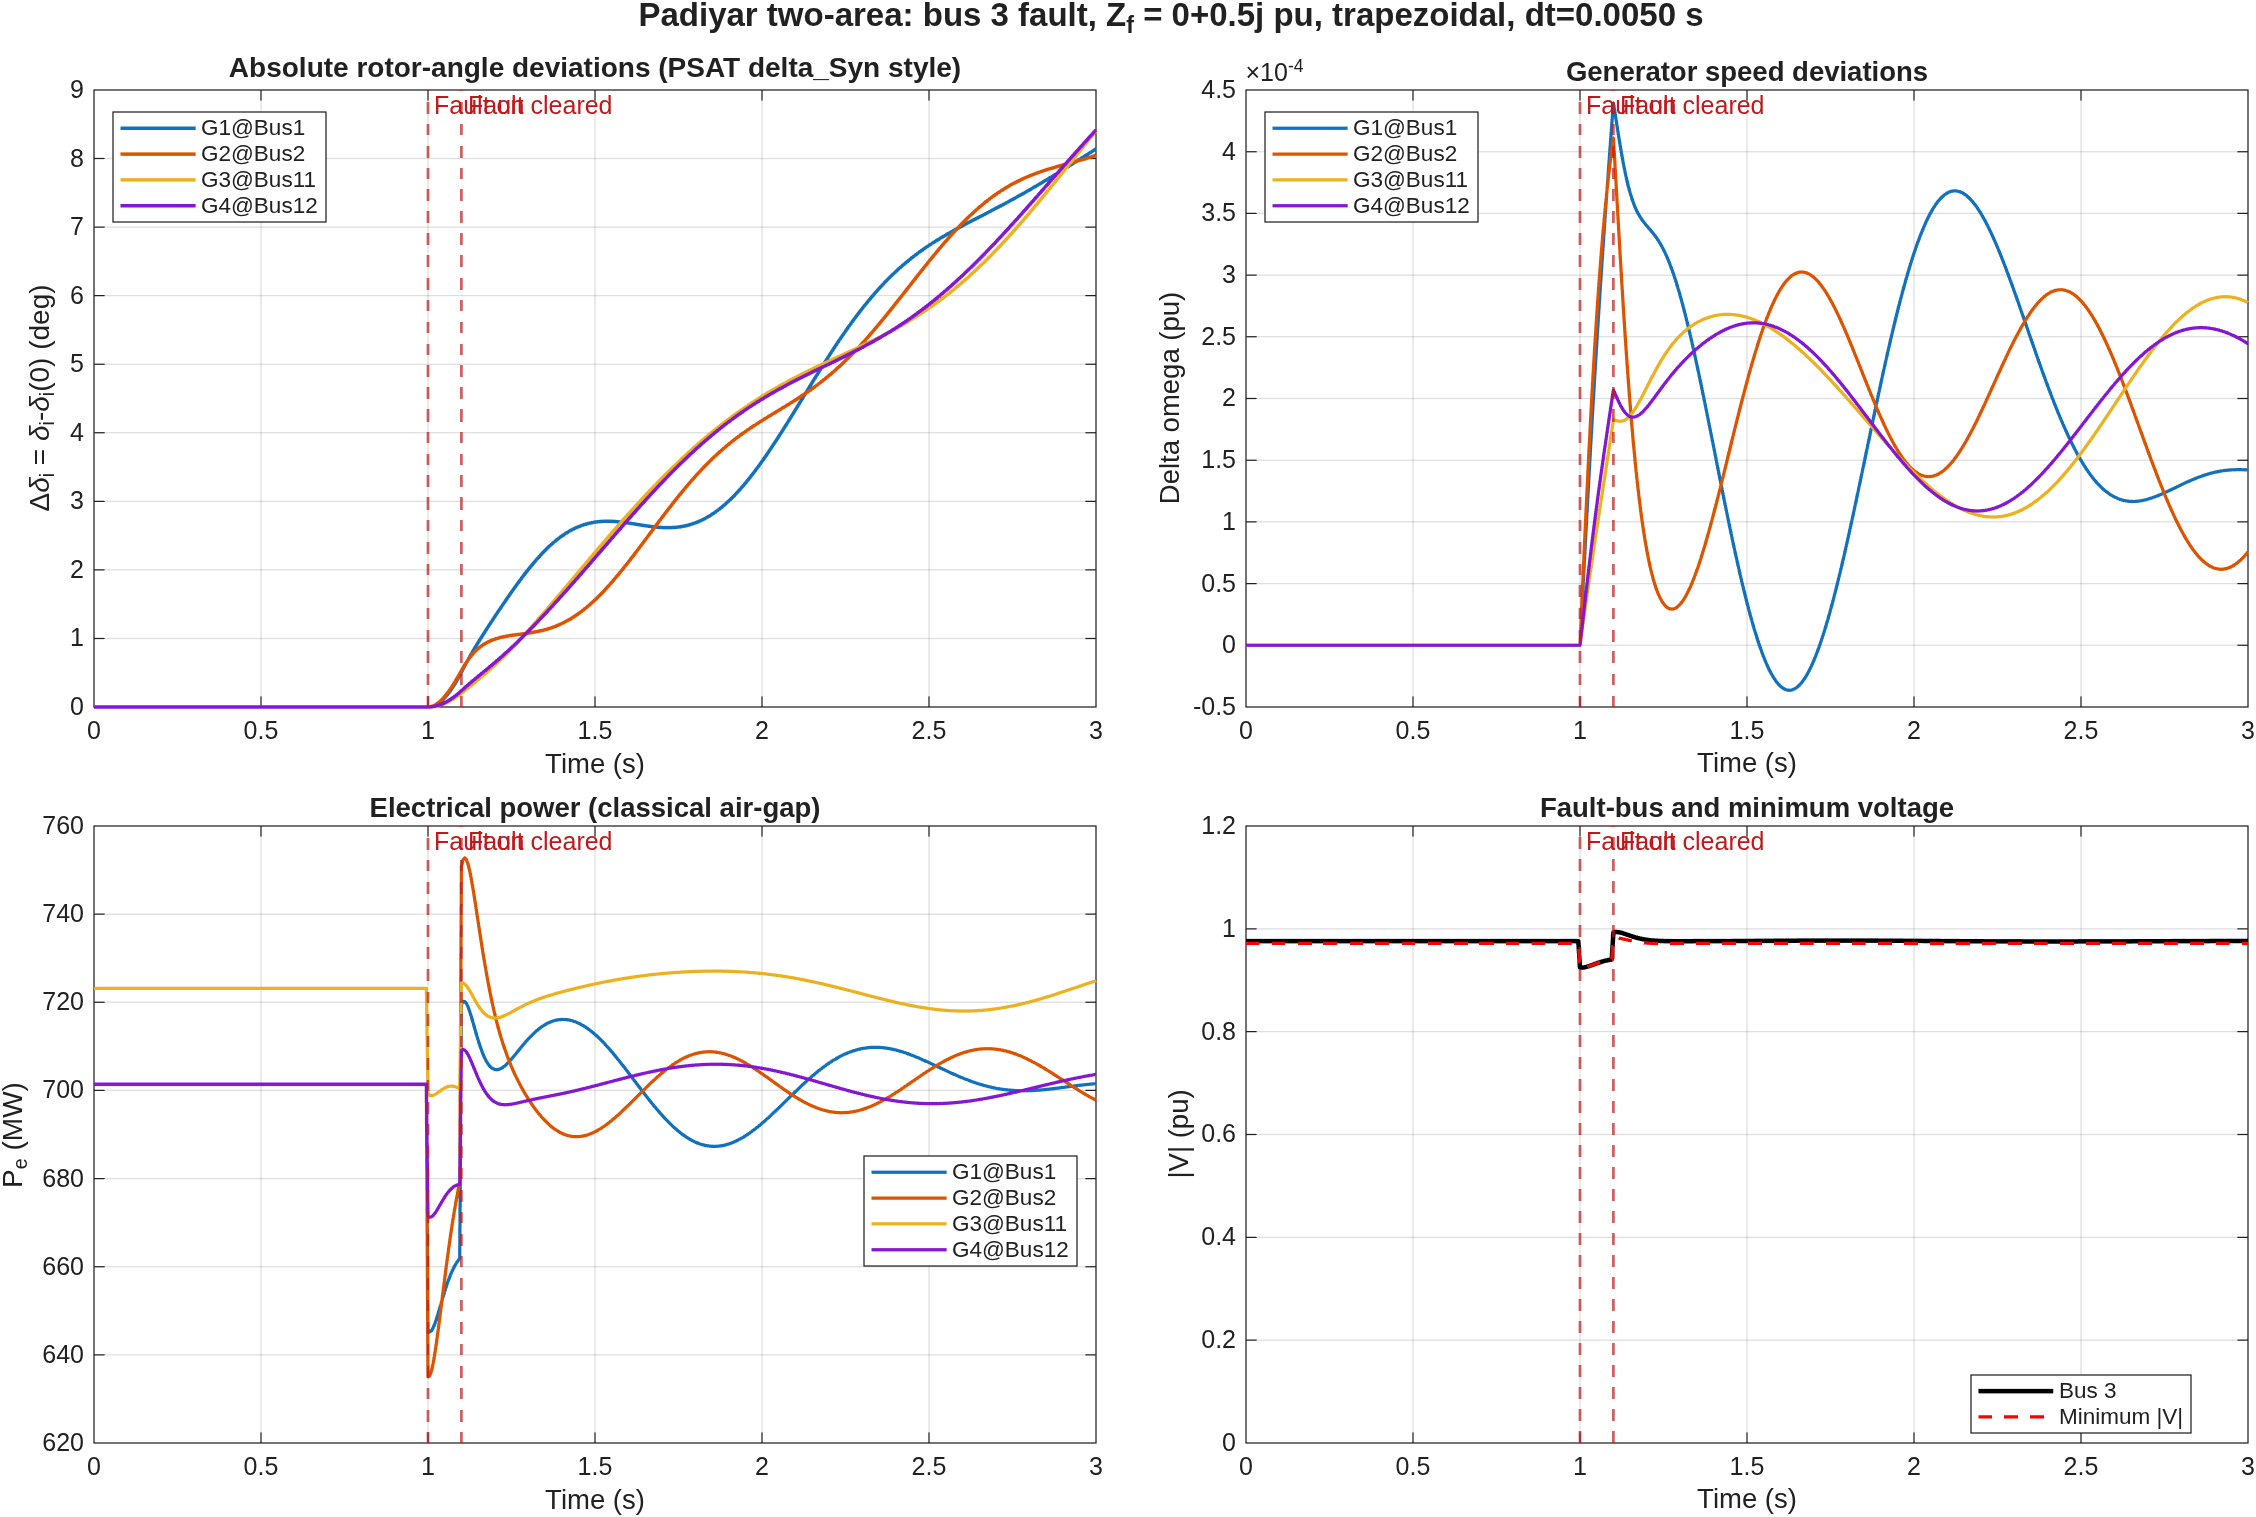
\includegraphics[width=.90\textwidth]{figures/padiyar_two_area/fault_comparison.png}
\caption{Bus-101 project fault response โดยใช้ AVR configuration (20-state model ของหนังสือ): stored absolute generator rotor angles $\delta_i(t)$ เป็น degrees ไม่มีการลบ initial-angle ออก เครื่องหมายสีแดงระบุ fault application และ clearance ช่วงจำลองคือ 0--20~s และ $Z_f=j10^{-4}$~pu}
\label{fig:ts-avr-angle}
\end{figure}

\begin{figure}[H]\centering
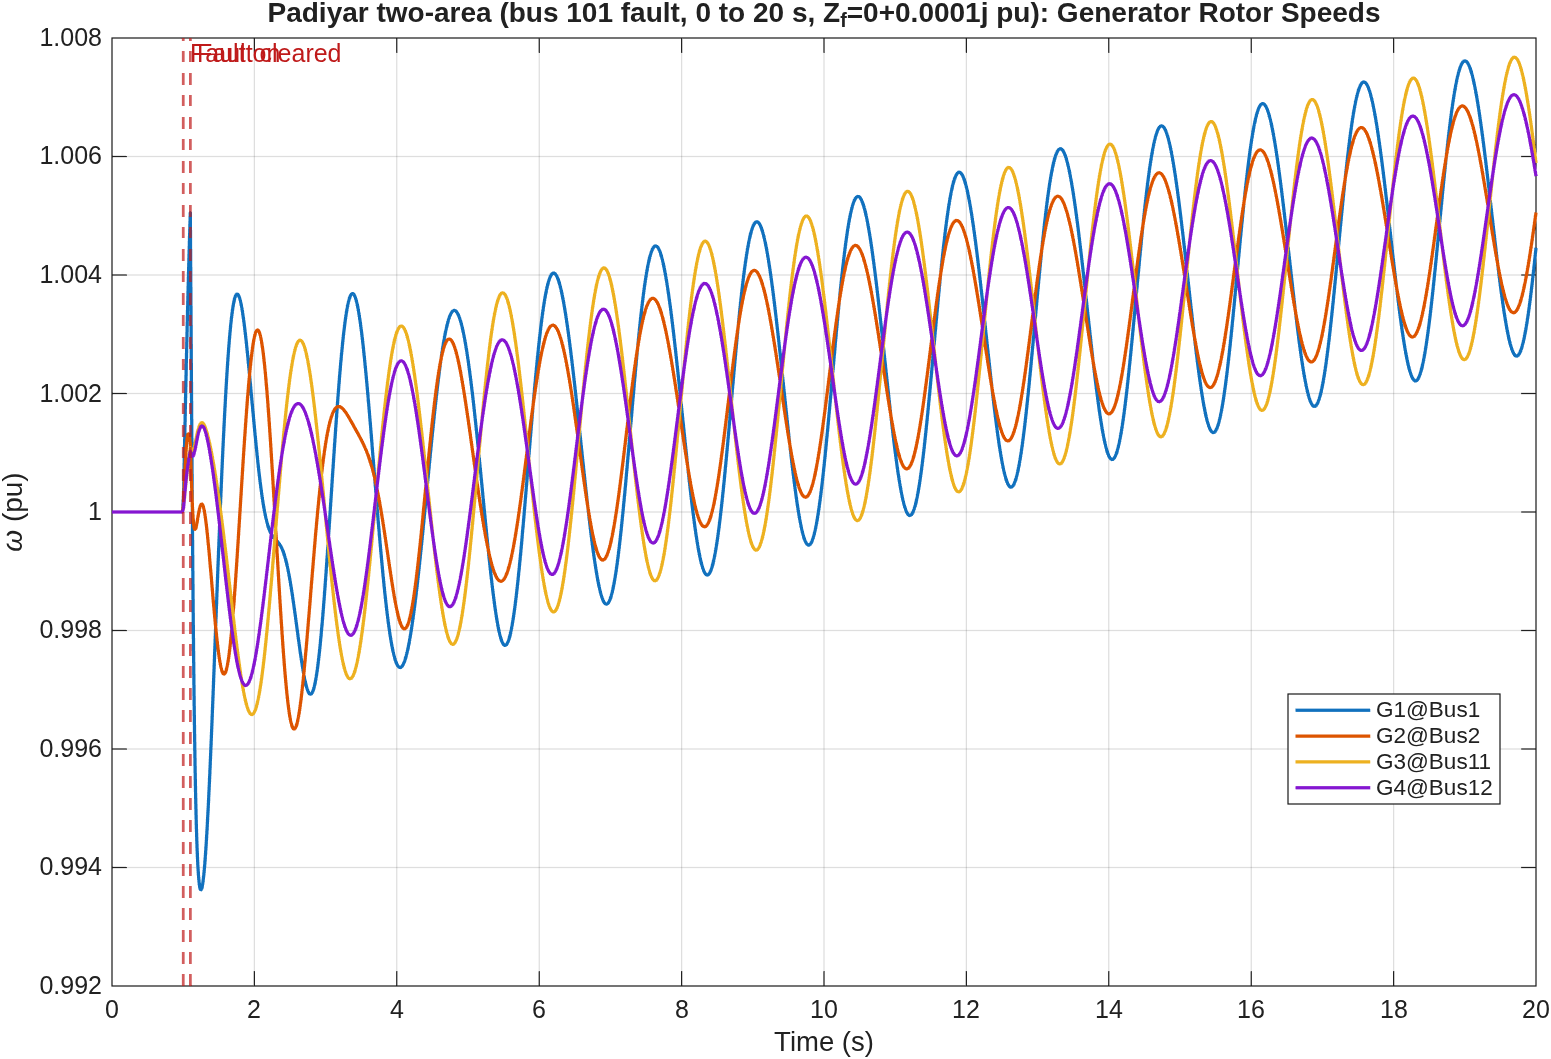
\includegraphics[width=.90\textwidth]{figures/padiyar_two_area/fault_comparison_omega.png}
\caption{Bus-101 project fault response โดยใช้ AVR configuration: stored absolute rotor speeds $\omega_i(t)$ ใน per unit ค่าที่ plot คือ TS result values เอง กราฟไม่ได้ plot $\omega_i-1$ ช่วงจำลองคือ 0--20~s และ $Z_f=j10^{-4}$~pu}
\label{fig:ts-avr-omega}
\end{figure}

\begin{figure}[H]\centering
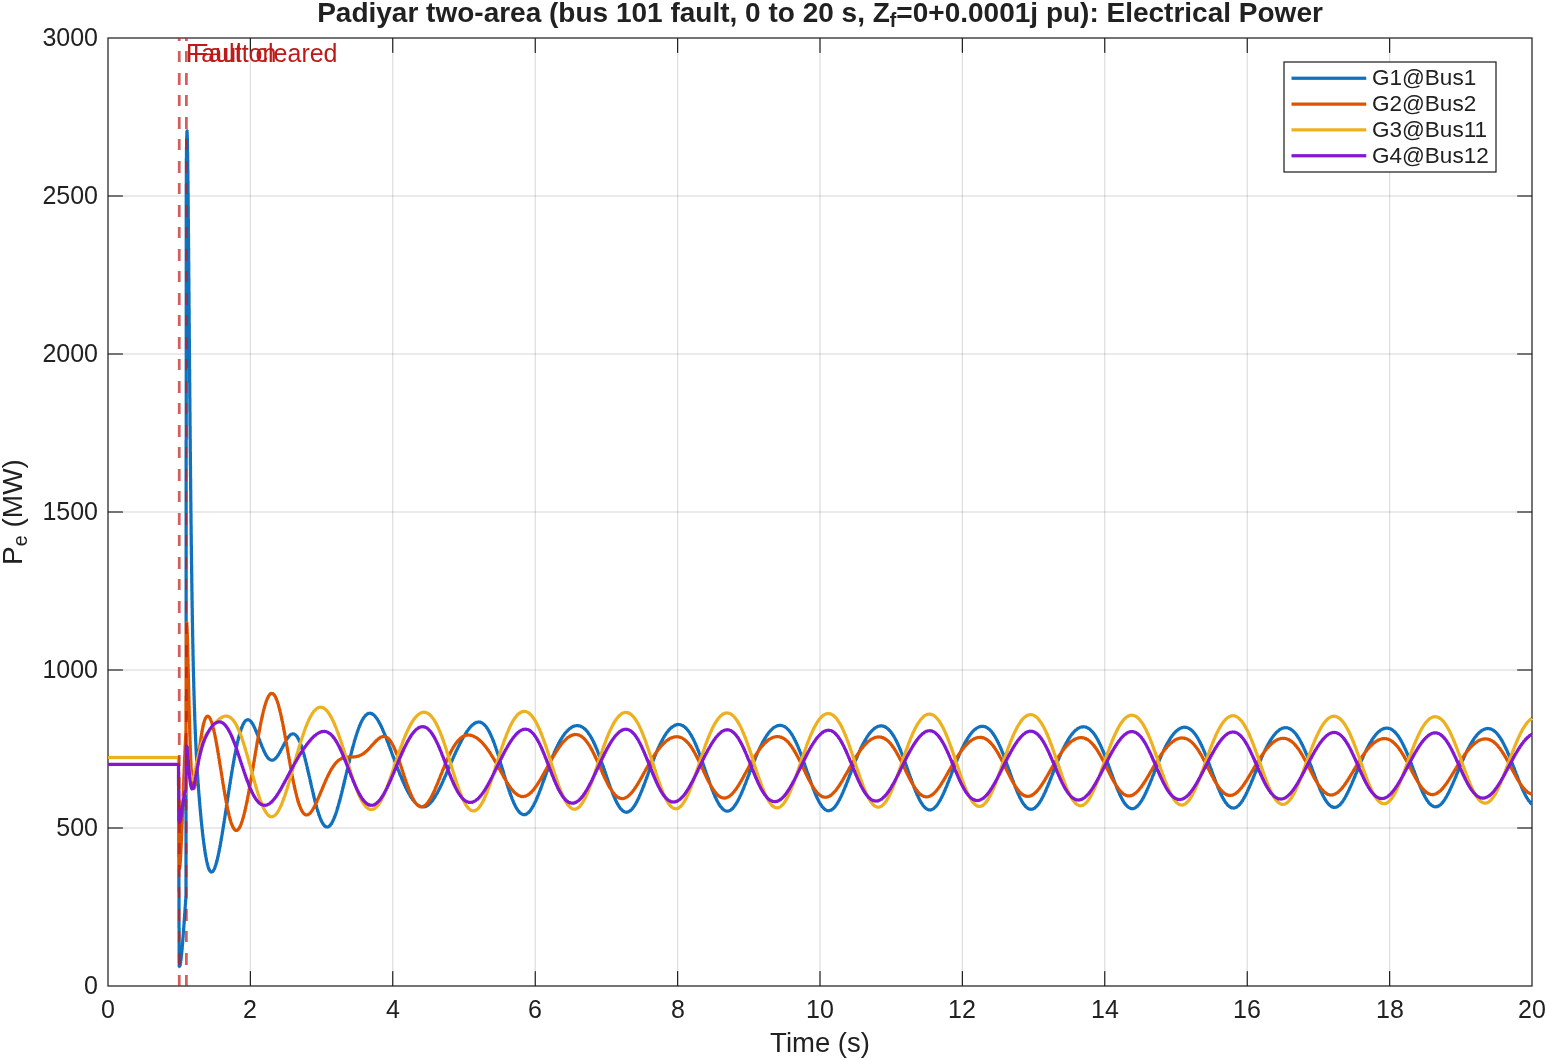
\includegraphics[width=.90\textwidth]{figures/padiyar_two_area/fault_comparison_pe.png}
\caption{Bus-101 project fault response โดยใช้ AVR configuration: generator air-gap electrical powers $P_{ei}(t)$ ที่ reconstruct จาก accepted TS states และ algebraic bus voltages ช่วงจำลองคือ 0--20~s และ $Z_f=j10^{-4}$~pu}
\label{fig:ts-avr-pe}
\end{figure}

\begin{figure}[H]\centering
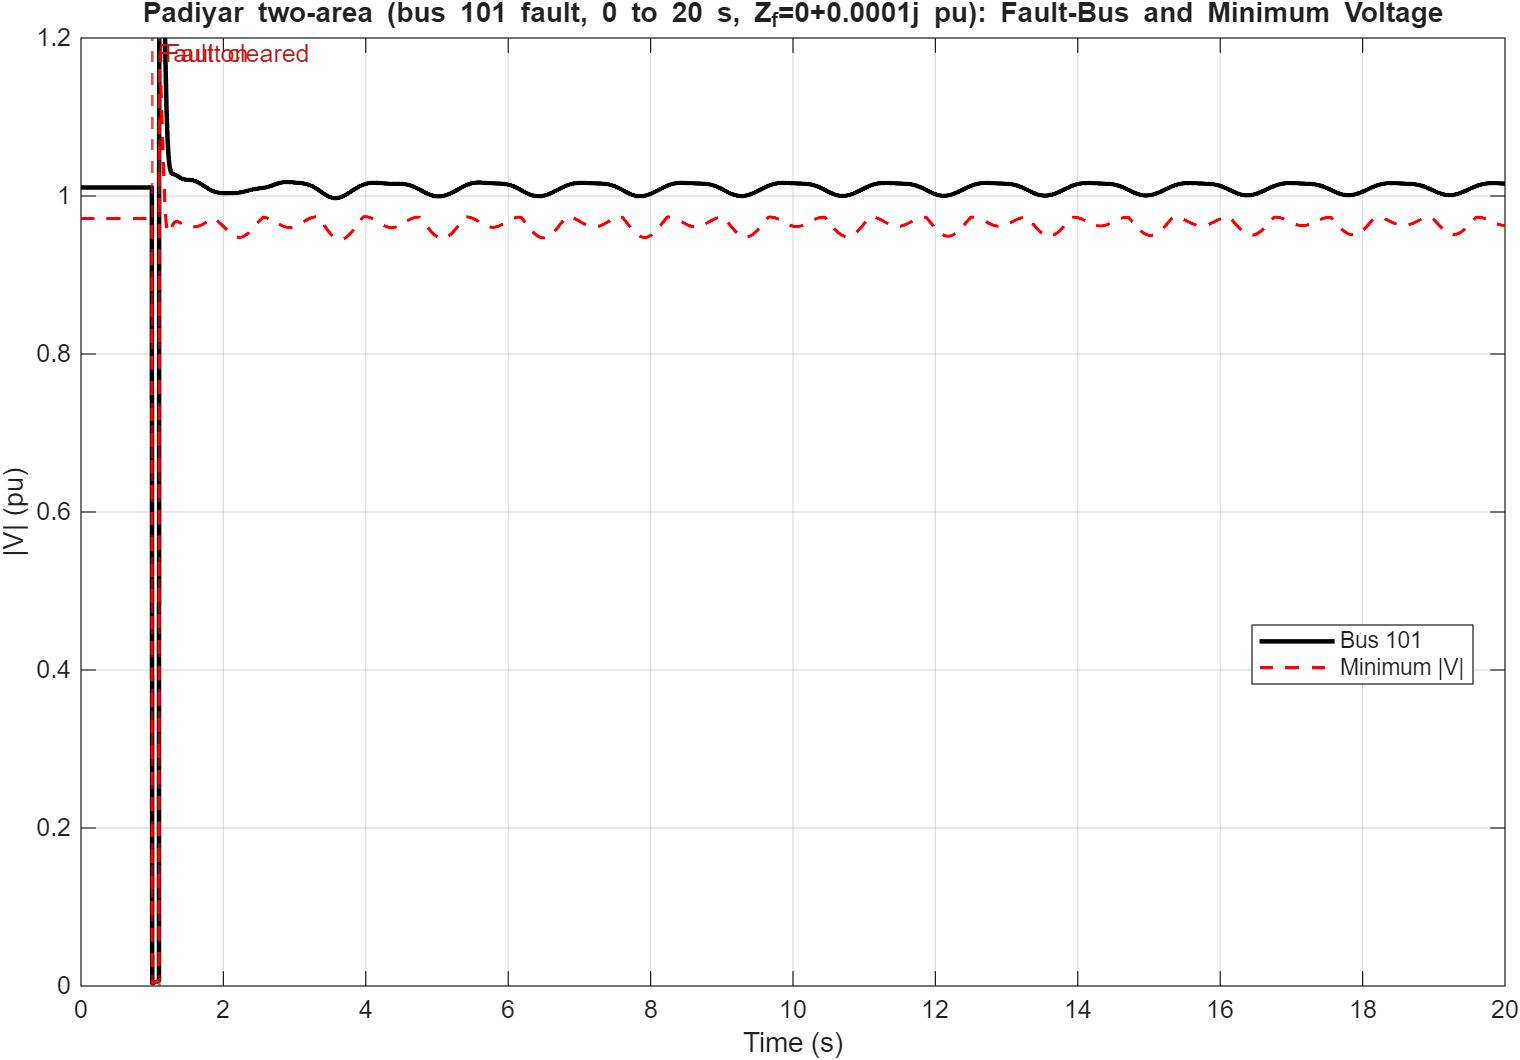
\includegraphics[width=.90\textwidth]{figures/padiyar_two_area/fault_comparison_voltage.png}
\caption{Bus-101 project fault response โดยใช้ AVR configuration: fault-bus voltage magnitude และ minimum voltage magnitude ทั่วทั้ง network ช่วงจำลองคือ 0--20~s และ $Z_f=j10^{-4}$~pu}
\label{fig:ts-avr-voltage}
\end{figure}

\begin{figure}[H]\centering
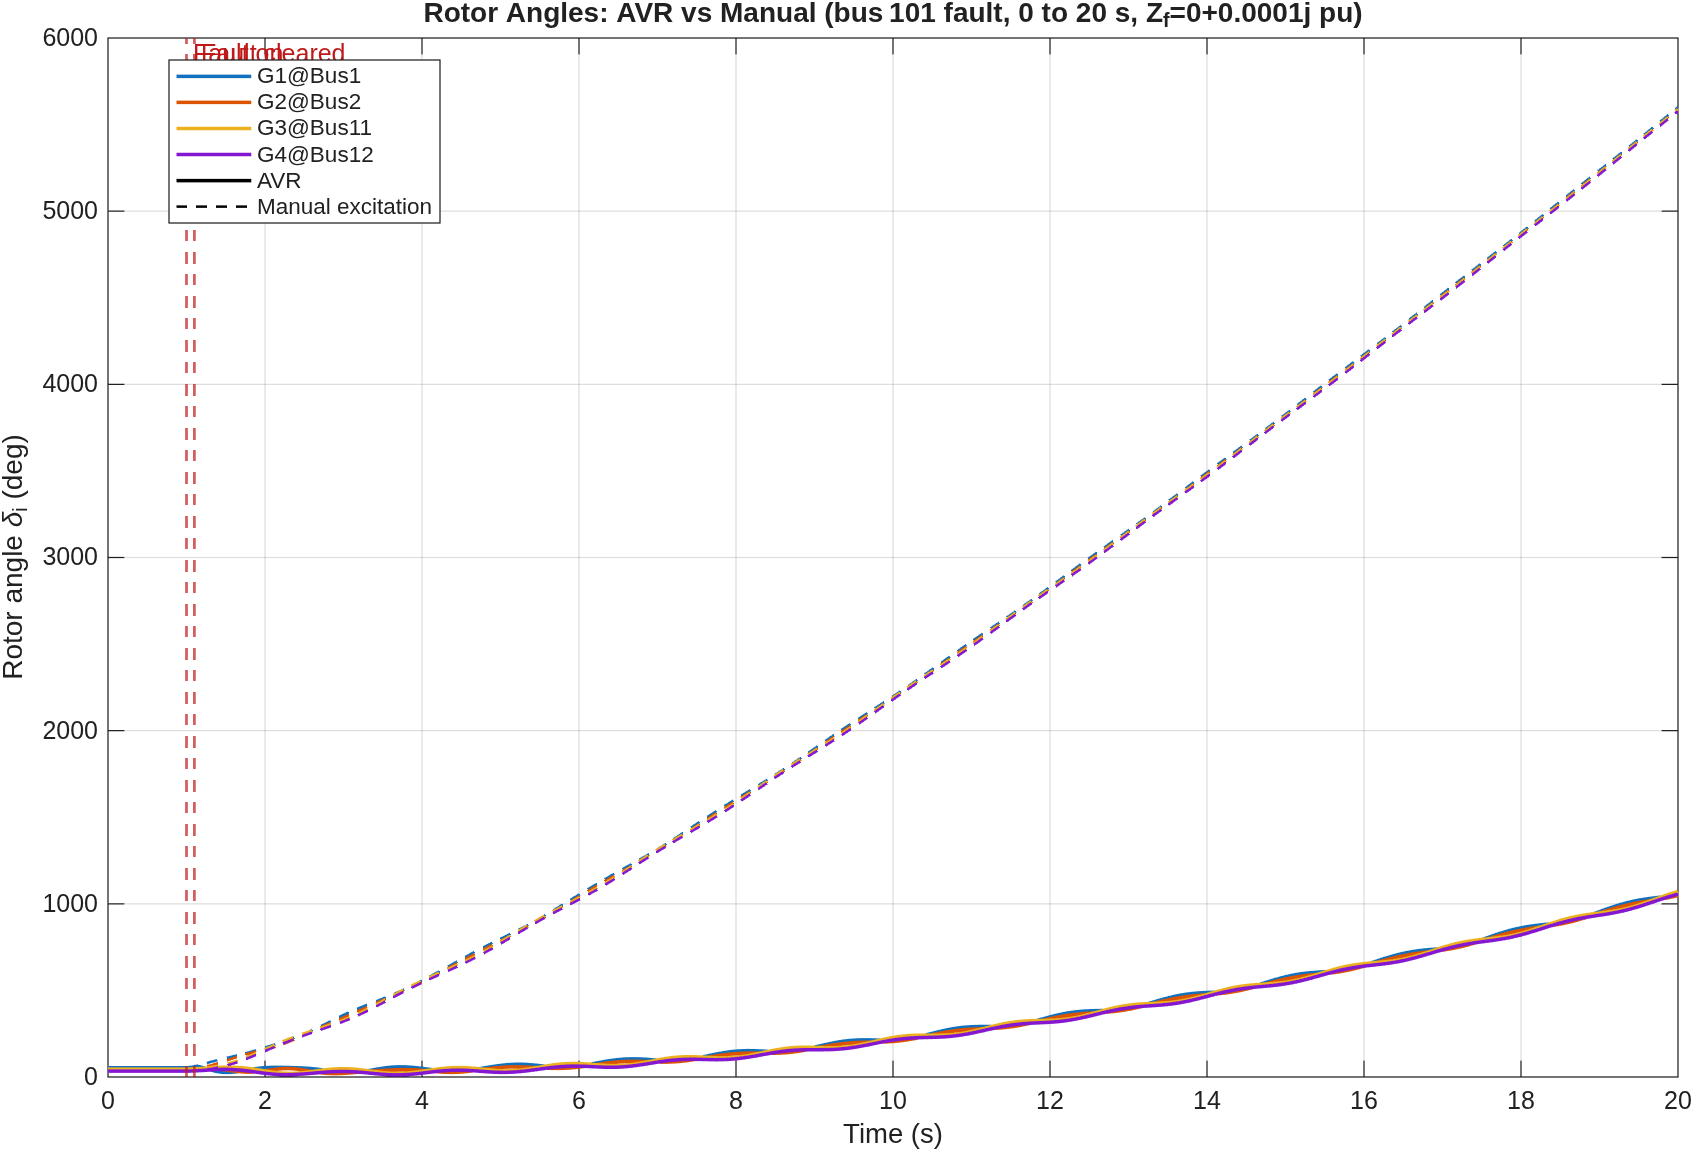
\includegraphics[width=.90\textwidth]{figures/padiyar_two_area/ts_avr_vs_manual.png}
\caption{Stored absolute rotor angles สำหรับ bus-101 fault: AVR (solid) เทียบกับ manual excitation (dashed) แต่ละสีระบุหนึ่ง generator ไม่มีการลบ initial-angle ออก ช่วงจำลองคือ 0--20~s และ $Z_f=j10^{-4}$~pu}
\label{fig:ts-comparison-angle}
\end{figure}

\begin{figure}[H]\centering
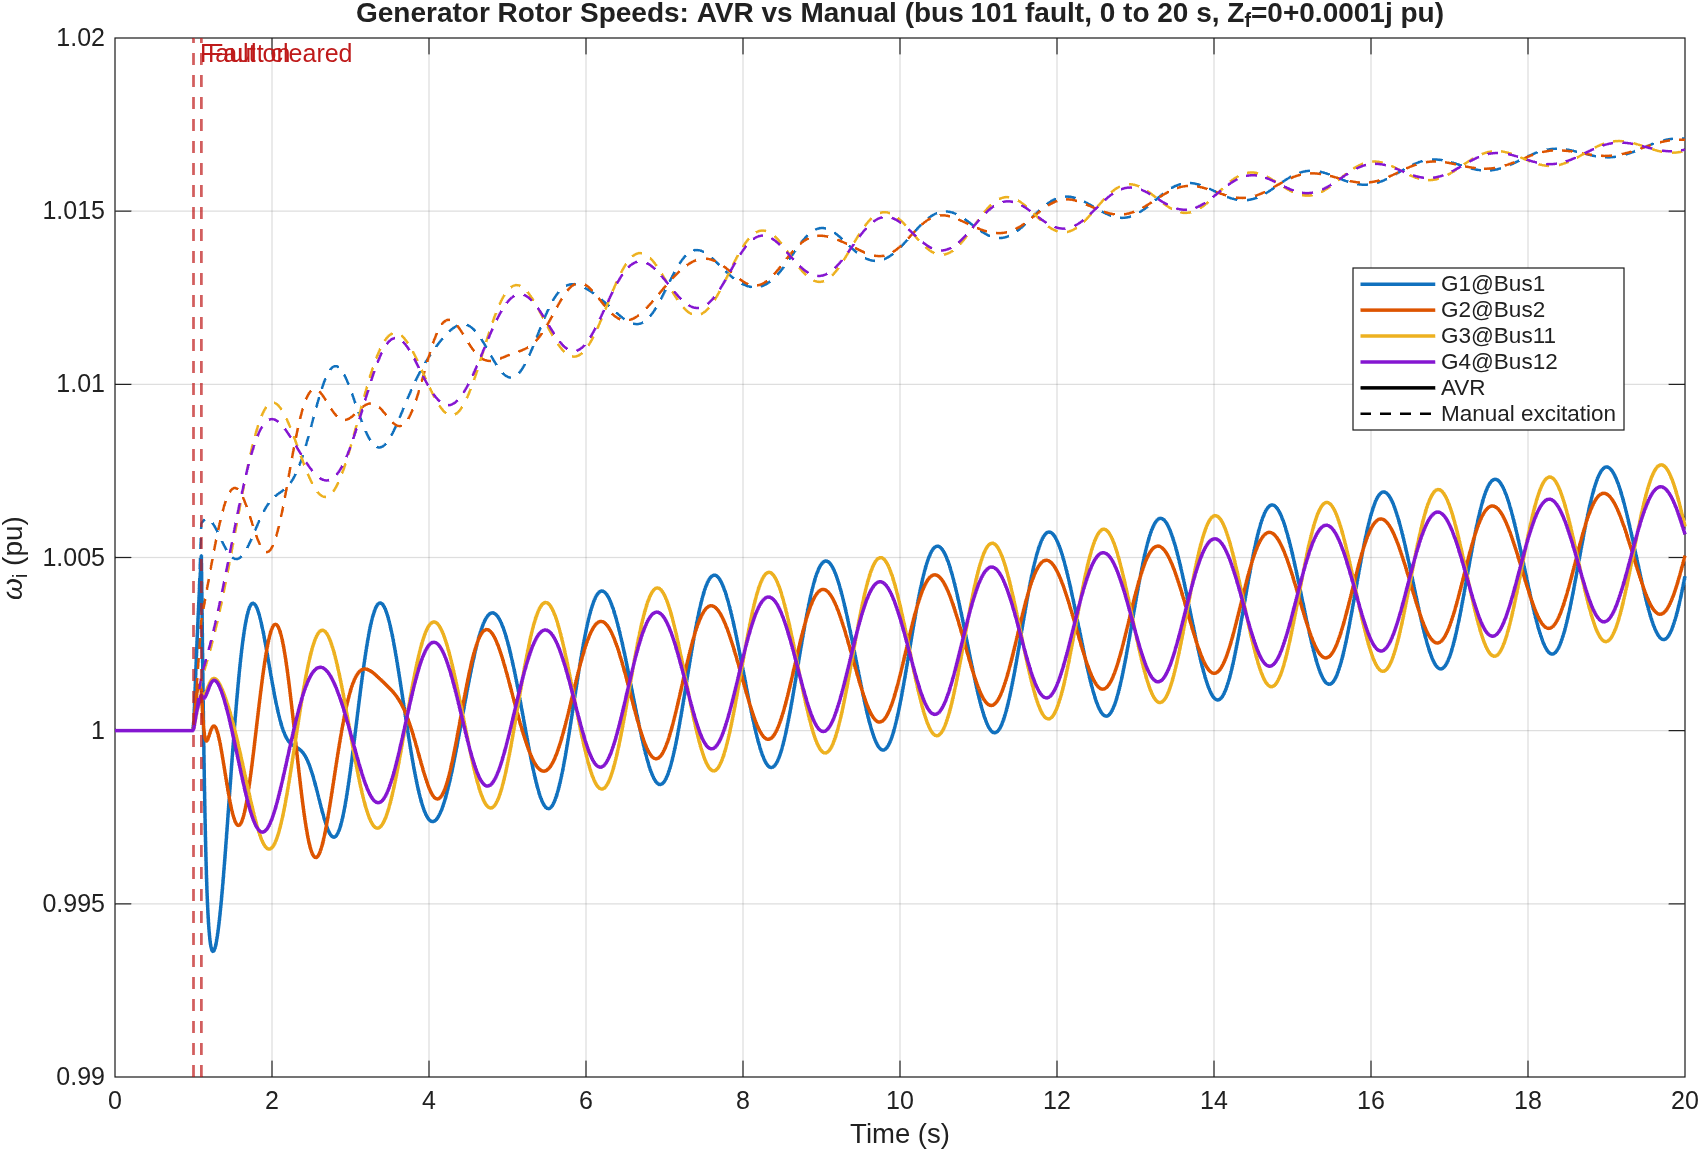
\includegraphics[width=.90\textwidth]{figures/padiyar_two_area/ts_avr_vs_manual_omega.png}
\caption{Stored absolute rotor speeds $\omega_i(t)$ สำหรับ bus-101 fault: AVR (solid) เทียบกับ manual excitation (dashed) ไม่มีการใช้ $\omega_i-1$ plotting transform ช่วงจำลองคือ 0--20~s และ $Z_f=j10^{-4}$~pu}
\label{fig:ts-comparison-omega}
\end{figure}

\begin{figure}[H]\centering
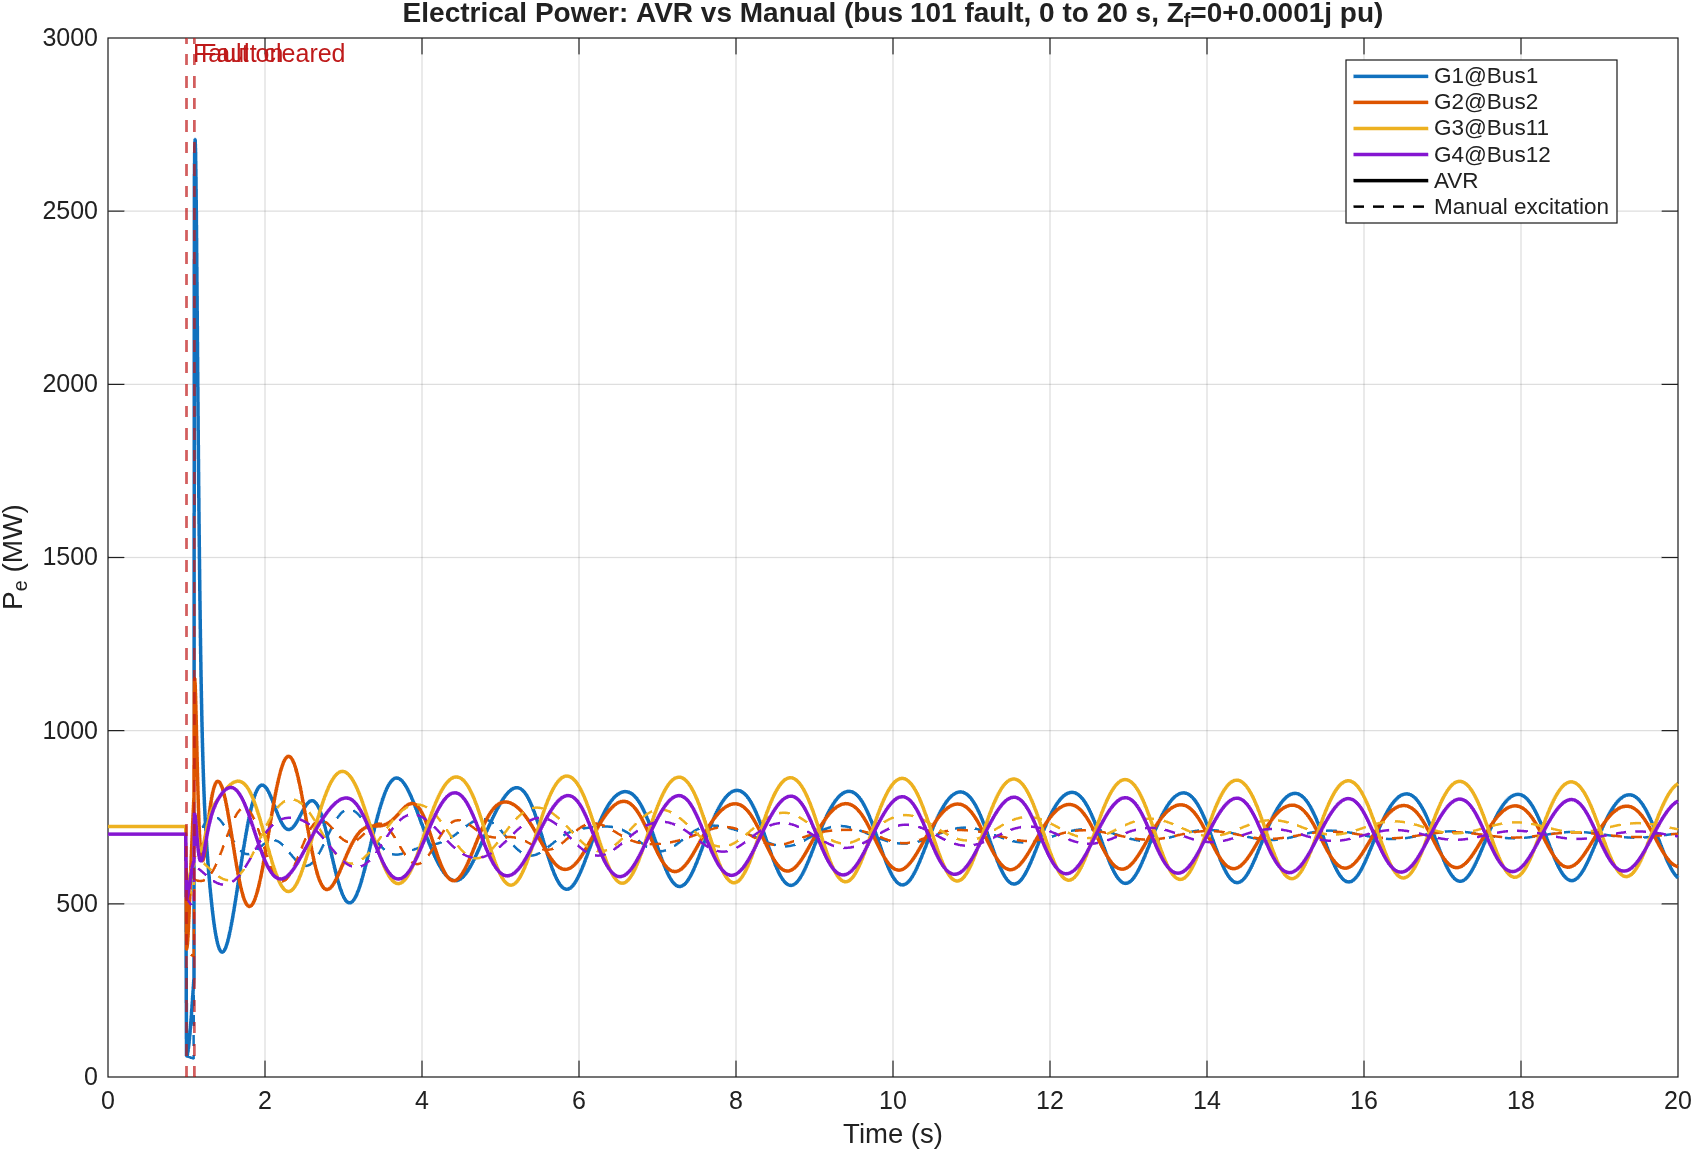
\includegraphics[width=.90\textwidth]{figures/padiyar_two_area/ts_avr_vs_manual_pe.png}
\caption{Generator electrical powers สำหรับ bus-101 fault: AVR (solid) เทียบกับ manual excitation (dashed) ช่วงจำลองคือ 0--20~s และ $Z_f=j10^{-4}$~pu}
\label{fig:ts-comparison-pe}
\end{figure}

\begin{figure}[H]\centering
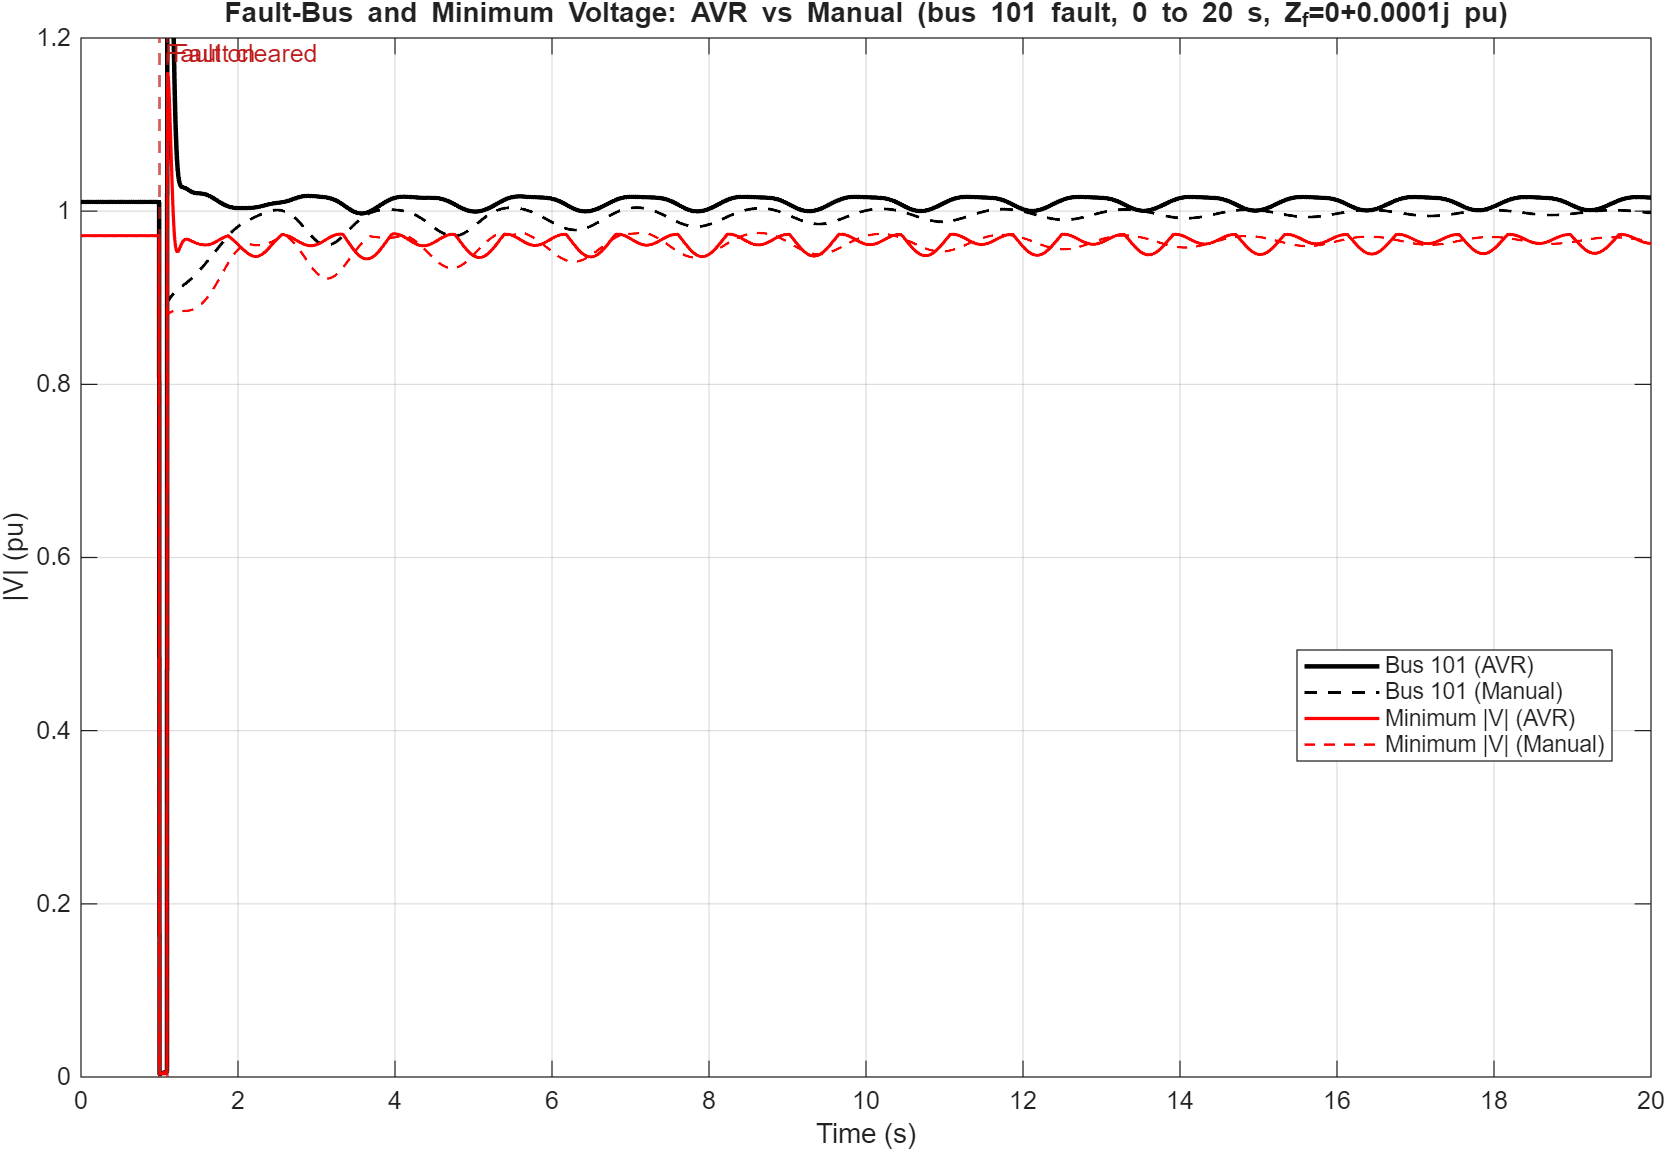
\includegraphics[width=.90\textwidth]{figures/padiyar_two_area/ts_avr_vs_manual_voltage.png}
\caption{Fault-bus และ minimum network voltage magnitudes สำหรับ bus-101 fault: AVR (solid) เทียบกับ manual excitation (dashed) ค่า quantitative modal damping ถูกกำหนดจาก \eqref{eq:sssa-modal-metrics} และ Table~10 ไม่ได้อนุมานจาก visual appearance ช่วงจำลองคือ 0--20~s และ $Z_f=j10^{-4}$~pu}
\label{fig:ts-comparison-voltage}
\end{figure}

\section{IEEE 14-bus Cross-validation เทียบกับ PSAT}

ส่วนนี้ cross-validate common classical PF, SSSA และ TDS substrate เทียบกับ PSAT~2.1.11 เป็น independent infrastructure check และไม่ใช่ claim ว่า PSAT implement five-state Padiyar model ที่ใช้ในหัวข้อก่อนหน้า ทุก IEEE14 tables และ figures ด้านล่างถูก generate ใน invocation เดียวกันเป็น fresh in-house run และ fresh PSAT run; ไม่มี saved trajectory, prior numeric table หรือ prior plot ถูกอ่าน จุดเข้า (entry point) คือ \path{generate_padiyar_ieee14_psat_tables}

\subsection{คำอธิบายระบบ (System Description)}

โครงข่ายคือ MATPOWER~6 IEEE 14-bus case ที่แปลงเป็น project schema มี 14 bus rows, 5 in-service generator rows ที่ buses 1, 2, 3, 6 และ 8 และ 20 in-service branch rows Input inventory ที่สมบูรณ์ที่ใช้ในการศึกษานี้ถูกให้ไว้ก่อน computed PF, SSSA และ TDS results

\begin{figure}[H]
\centering
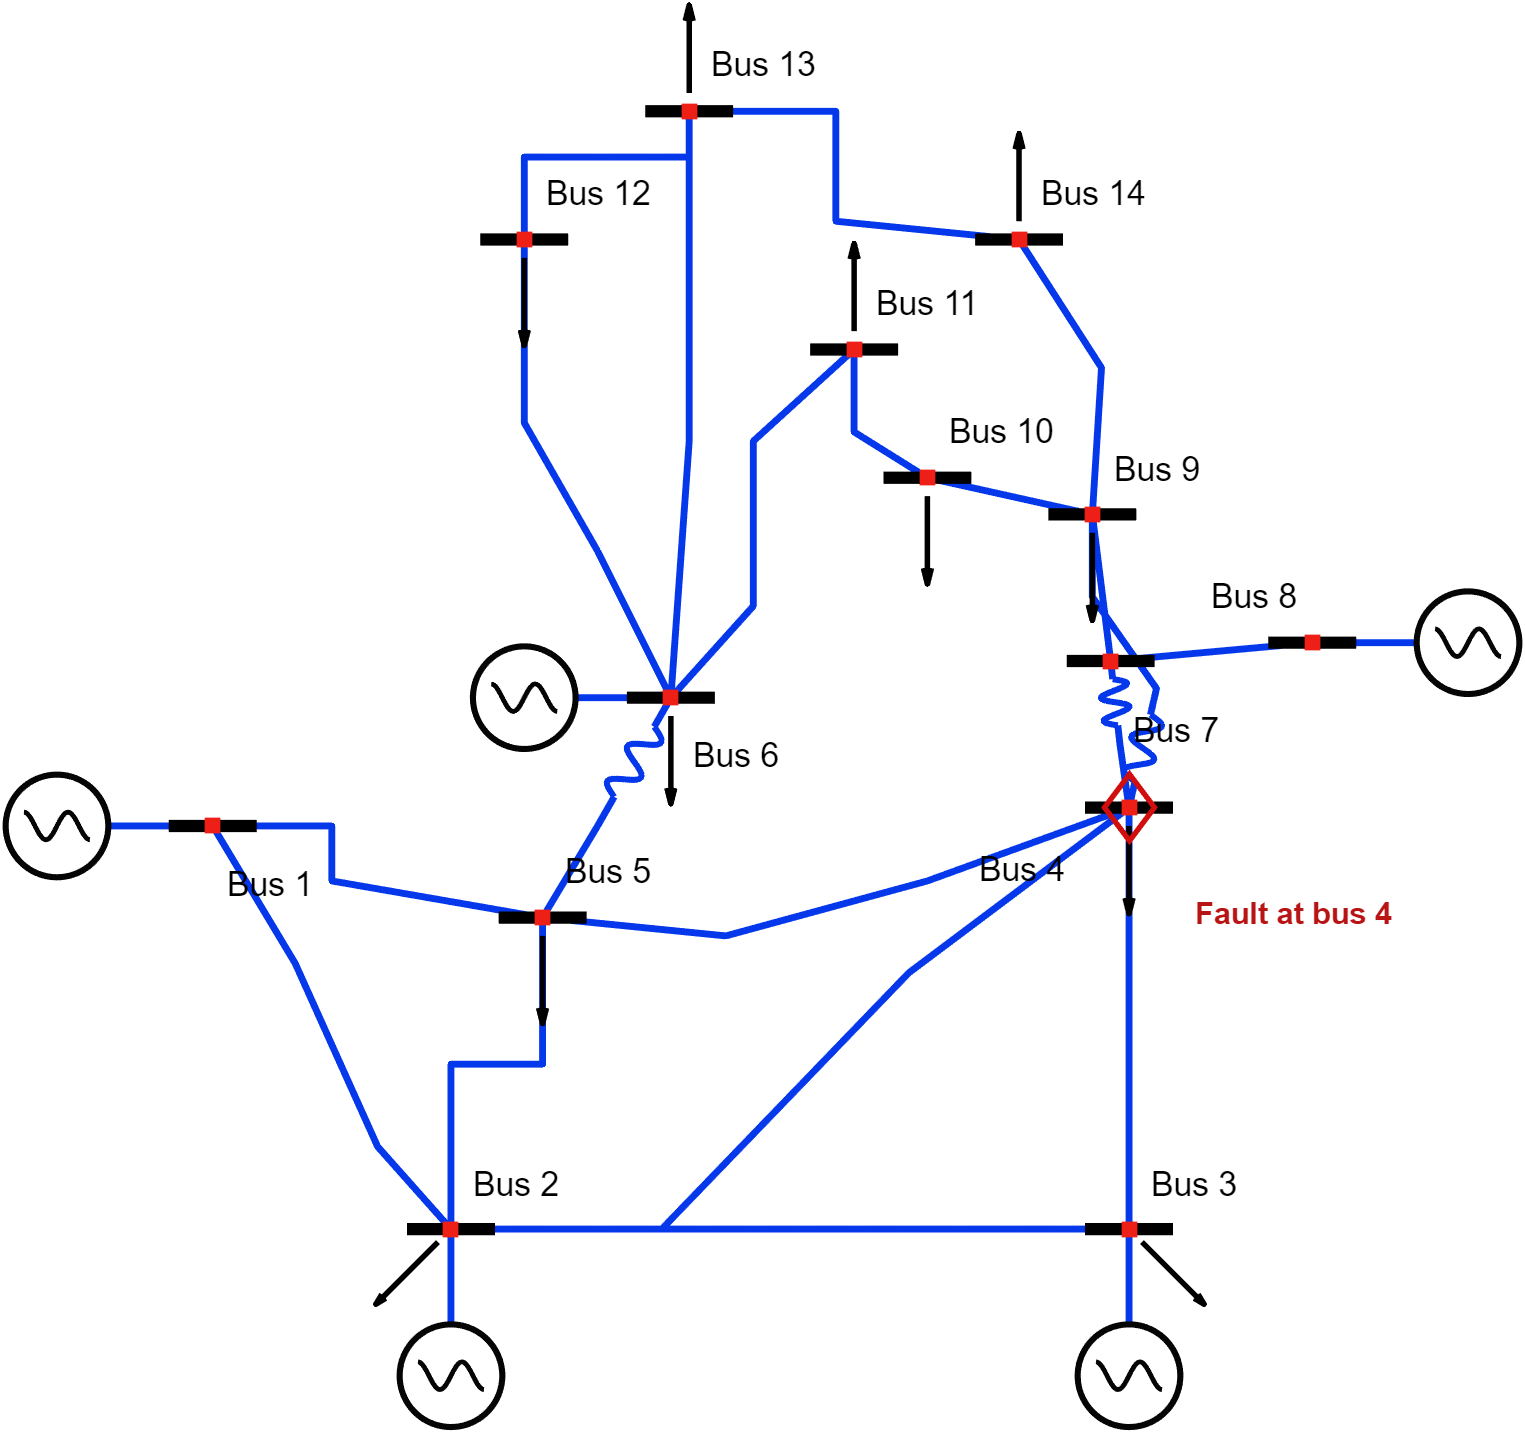
\includegraphics[width=.92\textwidth]{figures/padiyar_two_area/ieee14_network.png}
\caption{IEEE 14-bus network ที่ generate จาก MATPOWER branch, bus และ generator rows เดียวกันที่ใช้โดย Our และ PSAT มีการทำเครื่องหมาย generator buses, nonzero-load buses, transformer branches และ bus-4 fault location อย่างชัดแจ้ง}
\label{fig:ieee14-network}
\end{figure}

\subsection{Source Data (MATPOWER IEEE 14-bus)}

\begin{table}[H]\centering\small
\caption{MATPOWER IEEE14 case summary: 14 buses, 5 online generators และ 20 line/transformer rows พร้อม shared base quantities}
\label{tab:ieee14-case-summary}
\resizebox{\textwidth}{!}{% Fresh case summary derived from the exact IEEE14 case used by both solvers.
\begin{tabular}{lll}\toprule
Item & Value & Contract note \\ \midrule
Case & {MATPOWER 6.0 IEEE 14-bus} & Converted from the supplied case14.m \\ 
Power base & 100 MVA & MATPOWER mpc.baseMVA \\ 
Nominal frequency & 60 Hz & Project dynamic base \\ 
Bus rows & 14 & 1 REF, 4 PV, 9 PQ \\ 
Online generators & 5 & Buses [1,2,3,6,8] \\ 
Online branches & 20 & 3 transformer-tap branches \\ 
Total specified demand & 259.0 MW, 73.5 MVAr & Sum of bus Pd and Qd \\ 
Nonzero shunt susceptance & 19.0 MVAr & Bus 9 source Bs entry \\ 
\bottomrule\end{tabular}
}
\end{table}

\subsubsection{Bus Data และ Bus Types}

Table~\ref{tab:ieee14-bus-data} บันทึก source bus operating entries และ aggregated source generation ส่วน Table~\ref{tab:ieee14-bus-parameters} เก็บ remaining MATPOWER bus-matrix fields รวมถึง bus type, shunt, area, voltage limits และ initial voltage ค่า source $P_G/Q_G$ entries คือ case data; การตีความ input/output ของมันเป็นไปตาม effective REF, PV และ PQ bus types

\begin{table}[H]\centering\small
\caption{IEEE14 bus-type assignment รวมถึง MATPOWER type codes และ buses ในแต่ละ REF, PV และ PQ group}
\label{tab:ieee14-bus-types}
\resizebox{.78\textwidth}{!}{% Fresh bus-type assignment from the exact IEEE14 bus matrix.
\begin{tabular}{l r l r}\toprule
Bus type & MATPOWER code & Bus IDs & Count \\ \midrule
REF & 3 & {[1]} & 1 \\ 
PV & 2 & {[2,3,6,8]} & 4 \\ 
PQ & 1 & {[4,5,7,9,10,11,12,13,14]} & 9 \\ 
\bottomrule\end{tabular}
}
\end{table}

\begin{table}[H]\centering\small
\caption{IEEE 14-bus data และ bus types ที่ share กันโดย in-house และ PSAT runs}
\label{tab:ieee14-bus-data}
\resizebox{\textwidth}{!}{% Fresh source-data table generated in the same invocation as the IEEE14 simulations.
\begin{tabular}{r l r r r r r r}\toprule
Bus & Type & {$|V|_{src}$} & {$\theta_{src}$} & {$P_L$} & {$Q_L$} & {$P_G$} & {$Q_G$} \\
{} & {} & {(pu)} & {(deg)} & {(MW)} & {(MVAr)} & {(MW)} & {(MVAr)} \\ \midrule
1 & REF & 1.0600 & 0.0000 & 0.00 & 0.00 & 232.40 & -16.90 \\
2 & PV & 1.0450 & -4.9800 & 21.70 & 12.70 & 40.00 & 42.40 \\
3 & PV & 1.0100 & -12.7200 & 94.20 & 19.00 & 0.00 & 23.40 \\
4 & PQ & 1.0190 & -10.3300 & 47.80 & -3.90 & 0.00 & 0.00 \\
5 & PQ & 1.0200 & -8.7800 & 7.60 & 1.60 & 0.00 & 0.00 \\
6 & PV & 1.0700 & -14.2200 & 11.20 & 7.50 & 0.00 & 12.20 \\
7 & PQ & 1.0620 & -13.3700 & 0.00 & 0.00 & 0.00 & 0.00 \\
8 & PV & 1.0900 & -13.3600 & 0.00 & 0.00 & 0.00 & 17.40 \\
9 & PQ & 1.0560 & -14.9400 & 29.50 & 16.60 & 0.00 & 0.00 \\
10 & PQ & 1.0510 & -15.1000 & 9.00 & 5.80 & 0.00 & 0.00 \\
11 & PQ & 1.0570 & -14.7900 & 3.50 & 1.80 & 0.00 & 0.00 \\
12 & PQ & 1.0550 & -15.0700 & 6.10 & 1.60 & 0.00 & 0.00 \\
13 & PQ & 1.0500 & -15.1600 & 13.50 & 5.80 & 0.00 & 0.00 \\
14 & PQ & 1.0360 & -16.0400 & 14.90 & 5.00 & 0.00 & 0.00 \\
\bottomrule\end{tabular}
}
\end{table}

\begin{table}[H]\centering\scriptsize
\caption{MATPOWER IEEE14 bus data: complete bus-matrix parameters ที่จ่ายให้ case converter}
\label{tab:ieee14-bus-parameters}
\resizebox{\textwidth}{!}{% Fresh MATPOWER bus-matrix fields from the case used in this invocation.
\begin{tabular}{r l r r r r r r r r r r r}\toprule
Bus & Type & {$P_d$} & {$Q_d$} & {$G_s$} & {$B_s$} & Area & {$V_m$} & {$V_a$} & {baseKV} & Zone & {$V_{max}$} & {$V_{min}$} \\ 
{} & {} & {(MW)} & {(MVAr)} & {(MW)} & {(MVAr)} & {} & {(pu)} & {(deg)} & {(kV)} & {} & {(pu)} & {(pu)} \\ \midrule
1 & REF & 0.00 & 0.00 & 0.00 & 0.00 & 1 & 1.0600 & 0.0000 & 0.0 & 1 & 1.06 & 0.94 \\ 
2 & PV & 21.70 & 12.70 & 0.00 & 0.00 & 1 & 1.0450 & -4.9800 & 0.0 & 1 & 1.06 & 0.94 \\ 
3 & PV & 94.20 & 19.00 & 0.00 & 0.00 & 1 & 1.0100 & -12.7200 & 0.0 & 1 & 1.06 & 0.94 \\ 
4 & PQ & 47.80 & -3.90 & 0.00 & 0.00 & 1 & 1.0190 & -10.3300 & 0.0 & 1 & 1.06 & 0.94 \\ 
5 & PQ & 7.60 & 1.60 & 0.00 & 0.00 & 1 & 1.0200 & -8.7800 & 0.0 & 1 & 1.06 & 0.94 \\ 
6 & PV & 11.20 & 7.50 & 0.00 & 0.00 & 1 & 1.0700 & -14.2200 & 0.0 & 1 & 1.06 & 0.94 \\ 
7 & PQ & 0.00 & 0.00 & 0.00 & 0.00 & 1 & 1.0620 & -13.3700 & 0.0 & 1 & 1.06 & 0.94 \\ 
8 & PV & 0.00 & 0.00 & 0.00 & 0.00 & 1 & 1.0900 & -13.3600 & 0.0 & 1 & 1.06 & 0.94 \\ 
9 & PQ & 29.50 & 16.60 & 0.00 & 19.00 & 1 & 1.0560 & -14.9400 & 0.0 & 1 & 1.06 & 0.94 \\ 
10 & PQ & 9.00 & 5.80 & 0.00 & 0.00 & 1 & 1.0510 & -15.1000 & 0.0 & 1 & 1.06 & 0.94 \\ 
11 & PQ & 3.50 & 1.80 & 0.00 & 0.00 & 1 & 1.0570 & -14.7900 & 0.0 & 1 & 1.06 & 0.94 \\ 
12 & PQ & 6.10 & 1.60 & 0.00 & 0.00 & 1 & 1.0550 & -15.0700 & 0.0 & 1 & 1.06 & 0.94 \\ 
13 & PQ & 13.50 & 5.80 & 0.00 & 0.00 & 1 & 1.0500 & -15.1600 & 0.0 & 1 & 1.06 & 0.94 \\ 
14 & PQ & 14.90 & 5.00 & 0.00 & 0.00 & 1 & 1.0360 & -16.0400 & 0.0 & 1 & 1.06 & 0.94 \\ 
\bottomrule\end{tabular}
}
\end{table}

\subsubsection{Line Data}

ทั้ง 20 in-service MATPOWER line/transformer rows ถูก transcribe ใน Table~\ref{tab:ieee14-branch-data} ค่า zero source tap ratio หมายถึง MATPOWER unity-ratio default; ส่วนสาม nonzero ratios ระบุ transformer branches

\begin{table}[H]\centering\scriptsize
\caption{MATPOWER IEEE14 line และ transformer data (branch matrix); ทั้ง 20 rows อยู่ใน service}
\label{tab:ieee14-branch-data}
\resizebox{\textwidth}{!}{\input{figures/padiyar_two_area/table_ieee14_branch_data.tex}}
\end{table}

\subsubsection{Generator Data และ Dynamic Parameters}

5 online generator rows ถูก transcribe ใน Table~\ref{tab:ieee14-generator-data} ส่วน generator-cost rows ถูกเก็บไว้เพื่อ case completeness ใน Table~\ref{tab:ieee14-gencost} แม้ไม่มี optimal-power-flow calculation ที่ทำที่นี่

\begin{table}[H]\centering\scriptsize
\caption{MATPOWER IEEE14 online generator data}
\label{tab:ieee14-generator-data}
\resizebox{\textwidth}{!}{% Fresh MATPOWER online-generator fields from the case used in this invocation.
\begin{tabular}{r r r r r r r r r r r}\toprule
Gen & Bus & {$P_g$} & {$Q_g$} & {$Q_{max}$} & {$Q_{min}$} & {$V_g$} & {mBase} & Status & {$P_{max}$} & {$P_{min}$} \\ 
{} & {} & {(MW)} & {(MVAr)} & {(MVAr)} & {(MVAr)} & {(pu)} & {(MVA)} & {} & {(MW)} & {(MW)} \\ \midrule
1 & 1 & 232.40 & -16.90 & 10.00 & 0.00 & 1.0600 & 100.0 & 1 & 332.40 & 0.00 \\ 
2 & 2 & 40.00 & 42.40 & 50.00 & -40.00 & 1.0450 & 100.0 & 1 & 140.00 & 0.00 \\ 
3 & 3 & 0.00 & 23.40 & 40.00 & 0.00 & 1.0100 & 100.0 & 1 & 100.00 & 0.00 \\ 
4 & 6 & 0.00 & 12.20 & 24.00 & -6.00 & 1.0700 & 100.0 & 1 & 100.00 & 0.00 \\ 
5 & 8 & 0.00 & 17.40 & 24.00 & -6.00 & 1.0900 & 100.0 & 1 & 100.00 & 0.00 \\ 
\bottomrule\end{tabular}
}
\end{table}

\begin{table}[H]\centering\small
\caption{MATPOWER IEEE14 polynomial generator-cost data ที่ retain จาก source case}
\label{tab:ieee14-gencost}
\resizebox{.86\textwidth}{!}{% Fresh MATPOWER polynomial generation-cost rows from the same case.
\begin{tabular}{r r r r r r r r r}\toprule
Gen & Bus & Model & Startup & Shutdown & {$N$} & {$c_2$} & {$c_1$} & {$c_0$} \\ \midrule
1 & 1 & 2 & 0.0 & 0.0 & 3 & 0.0430292599 & 20 & 0 \\ 
2 & 2 & 2 & 0.0 & 0.0 & 3 & 0.25 & 20 & 0 \\ 
3 & 3 & 2 & 0.0 & 0.0 & 3 & 0.01 & 40 & 0 \\ 
4 & 6 & 2 & 0.0 & 0.0 & 3 & 0.01 & 40 & 0 \\ 
5 & 8 & 2 & 0.0 & 0.0 & 3 & 0.01 & 40 & 0 \\ 
\bottomrule\end{tabular}
}
\end{table}

Static MATPOWER case ไม่ได้ให้ complete dynamic data set ดังนั้น 5 classical-machine rows ใน Table~\ref{tab:ieee14-machine-data} จึงถูก label อย่างชัดแจ้งว่า \texttt{ASSUMED\_DIAGNOSTIC}; identical rows ถูกส่งให้ทั้ง Our และ PSAT

\begin{table}[H]\centering\small
\caption{Classical-machine parameters ที่ใช้เหมือนกันโดย Our และ PSAT}
\label{tab:ieee14-machine-data}
\resizebox{.86\textwidth}{!}{% Fresh dynamic-machine contract applied identically to Our and PSAT.
\begin{tabular}{r r r r r l}\toprule
Machine & Bus & {$H$ (s)} & {$D$ (pu)} & {$X'_d$ (pu)} & Provenance \\ \midrule
1 & 1 & 5.00 & 0.00 & 0.300 & {ASSUMED\_DIAGNOSTIC} \\ 
2 & 2 & 5.00 & 0.00 & 0.300 & {ASSUMED\_DIAGNOSTIC} \\ 
3 & 3 & 5.00 & 0.00 & 0.300 & {ASSUMED\_DIAGNOSTIC} \\ 
4 & 6 & 5.00 & 0.00 & 0.300 & {ASSUMED\_DIAGNOSTIC} \\ 
5 & 8 & 5.00 & 0.00 & 0.300 & {ASSUMED\_DIAGNOSTIC} \\ 
\bottomrule\end{tabular}
}
\end{table}

\subsubsection{Fault และ Simulation Inputs}

Identical event contract ใน Table~\ref{tab:ieee14-scenario} ใช้ balanced three-phase fault ที่ bus~4 ด้วย $Z_f=j10^{-4}$~pu ใช้ที่ 1.0~s และ clear ที่ 1.1~s ทั้งสอง simulations รันถึง 15~s ด้วย nominal 0.01~s step

\begin{table}[H]\centering\small
\caption{Identical IEEE14 model และ event inputs ที่ supply ให้ทั้ง Our และ PSAT}
\label{tab:ieee14-scenario}
\resizebox{\textwidth}{!}{% Fresh identical-input contract for Our and PSAT.
\begin{tabular}{lcc}\toprule
Input & Our & PSAT \\ \midrule
Network & MATPOWER 6 IEEE14 & Converted from the same case \\
Generator buses & {[1,2,3,6,8]} & {[1,2,3,6,8]} \\
Classical dynamics $(H,D,X'_d)$ & $(5,0,0.3)$ & $(5,0,0.3)$ \\
Fault bus & 4 & 4 \\
Fault impedance $Z_f$ (pu) & {$j10^{-4}$} & {$j10^{-4}$} \\
Fault interval (s) & 1.0--1.1 & 1.0--1.1 \\
Simulation horizon (s) & 15 & 15 \\
Nominal step (s) & 0.01 & 0.01 \\
\bottomrule\end{tabular}
}
\end{table}

\subsection{Power-flow Results}

Table~\ref{tab:ieee14-pf} รายงานทั้ง solved bus-voltage columns โดยตรง ด้วย bus IDs map ก่อน subtraction PSAT ได้รับ network ผ่าน project converter แทนที่จะผ่าน unrelated built-in case

\begin{table}[H]\centering\small
\caption{Fresh IEEE14 power-flow comparison: Our เทียบกับ PSAT}
\label{tab:ieee14-pf}
\resizebox{\textwidth}{!}{% Fresh Our and PSAT PF results; no saved result was read.
\begin{tabular}{r rr rr rr}\toprule
& \multicolumn{2}{c}{Our} & \multicolumn{2}{c}{PSAT} & \multicolumn{2}{c}{Absolute difference} \\ 
Bus & {$|V|$} & {$\theta$} & {$|V|$} & {$\theta$} & {$|\Delta V|$} & {$|\Delta\theta|$} \\ 
{} & {(pu)} & {(deg)} & {(pu)} & {(deg)} & {(pu)} & {(deg)} \\ \midrule
1 & 1.060000 & 0.000000 & 1.060000 & 0.000000 & 0.00e+00 & 0.00e+00 \\
2 & 1.045000 & -4.982589 & 1.045000 & -4.982589 & 0.00e+00 & 2.66e-15 \\
3 & 1.010000 & -12.725100 & 1.010000 & -12.725100 & 0.00e+00 & 1.78e-15 \\
4 & 1.017671 & -10.312901 & 1.017671 & -10.312901 & 0.00e+00 & 1.78e-15 \\
5 & 1.019514 & -8.773854 & 1.019514 & -8.773854 & 2.22e-16 & 5.33e-15 \\
6 & 1.070000 & -14.220946 & 1.070000 & -14.220946 & 0.00e+00 & 1.95e-14 \\
7 & 1.061520 & -13.359627 & 1.061520 & -13.359627 & 0.00e+00 & 1.78e-15 \\
8 & 1.090000 & -13.359627 & 1.090000 & -13.359627 & 0.00e+00 & 3.55e-15 \\
9 & 1.055932 & -14.938521 & 1.055932 & -14.938521 & 4.44e-16 & 8.88e-15 \\
10 & 1.050985 & -15.097288 & 1.050985 & -15.097288 & 6.66e-16 & 1.24e-14 \\
11 & 1.056907 & -14.790622 & 1.056907 & -14.790622 & 4.44e-16 & 1.95e-14 \\
12 & 1.055189 & -15.075585 & 1.055189 & -15.075585 & 2.22e-16 & 2.84e-14 \\
13 & 1.050382 & -15.156276 & 1.050382 & -15.156276 & 4.44e-16 & 2.84e-14 \\
14 & 1.035530 & -16.033645 & 1.035530 & -16.033645 & 6.66e-16 & 1.42e-14 \\
\bottomrule\end{tabular}
}
\end{table}

\begin{figure}[H]\centering
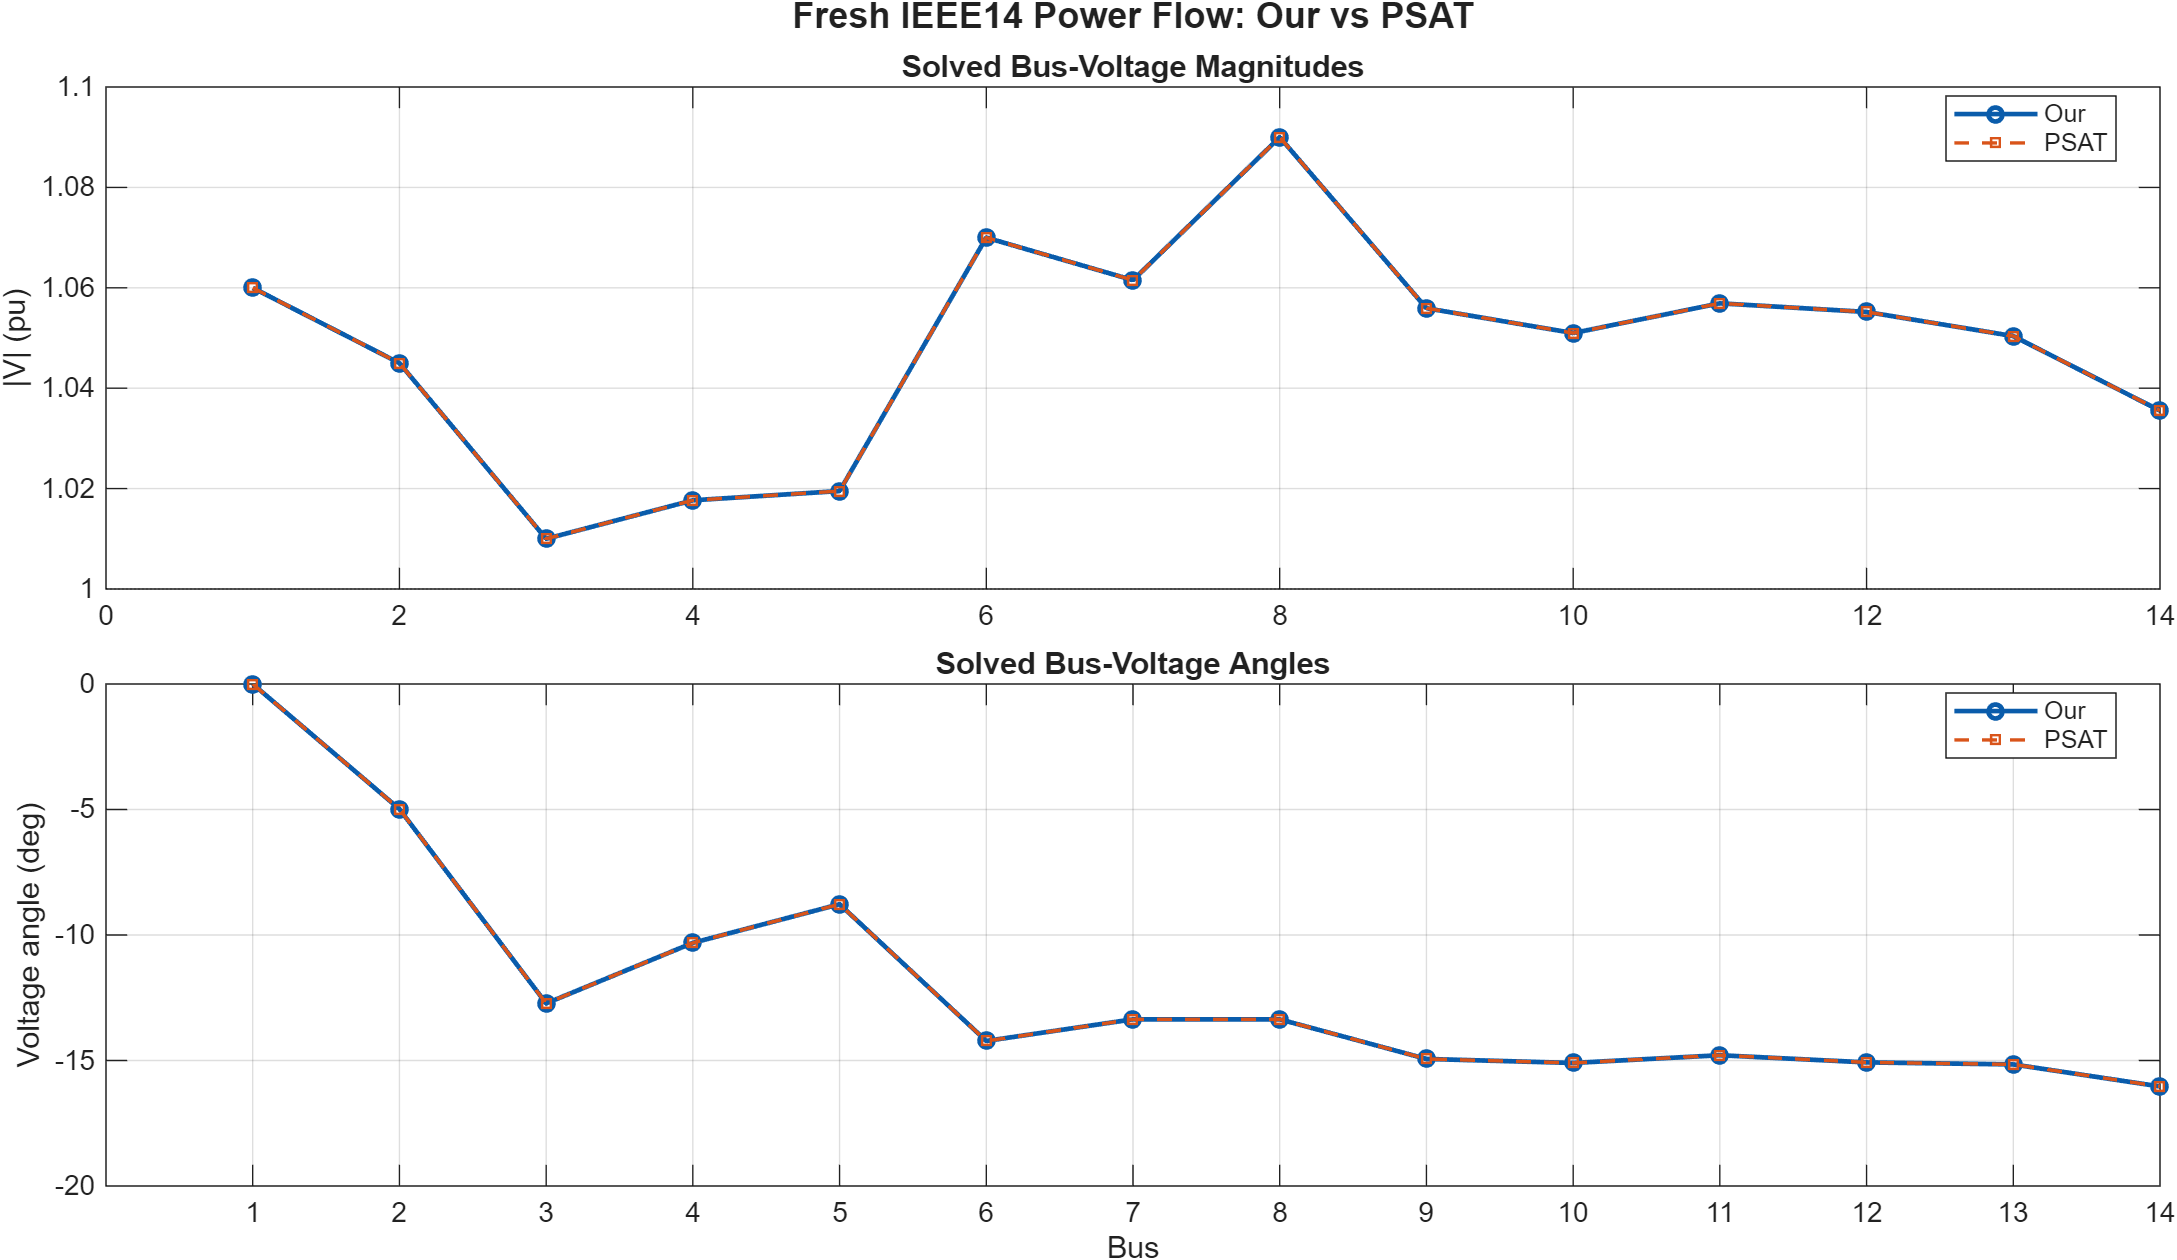
\includegraphics[width=.94\textwidth]{figures/padiyar_two_area/ieee14_pf_ours_psat.png}
\caption{Fresh IEEE14 solved bus-voltage magnitudes และ angles ของเราเป็น solid และ PSAT เป็น dashed; ทั้งสอง traces ใช้ bus-ID mapping ที่รายงานใน Table~\ref{tab:ieee14-pf}}
\label{fig:ieee14-pf-solution}
\end{figure}

\begin{figure}[H]\centering
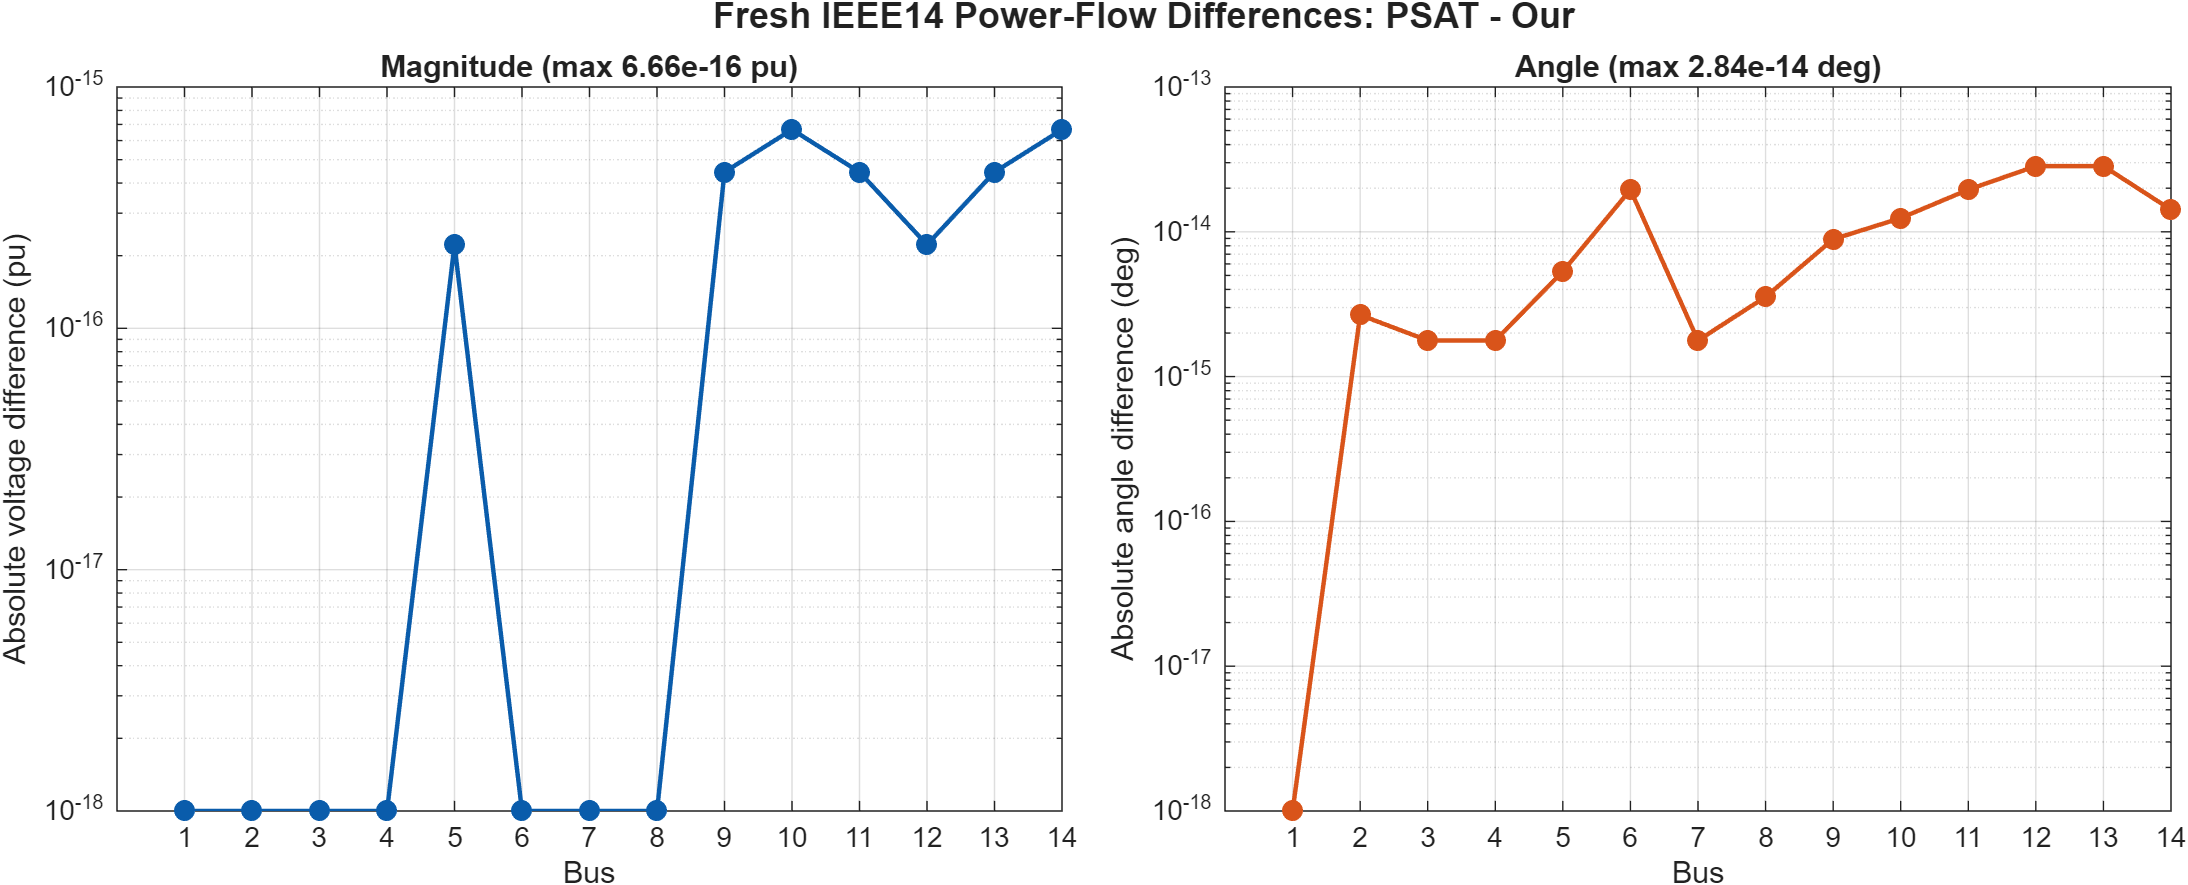
\includegraphics[width=.94\textwidth]{figures/padiyar_two_area/ieee14_pf_error_ours_psat.png}
\caption{Per-bus absolute PF differences จาก fresh Our และ PSAT solutions เดียวกัน ค่า zero differences ถูกแสดงที่ numerical display floor บน logarithmic axes}
\label{fig:ieee14-pf-error}
\end{figure}

\subsection{Small-Signal Stability Results}

Table~\ref{tab:ieee14-sssa} เปรียบเทียบ positive-imaginary physical relative modes จาก identical five-machine classical model ส่วน common-angle zero mode ถูก omit โดย declared $10^{-3}$~rad/s frequency threshold ค่า PSAT ถูกรายงานตรงตามที่ได้จาก state-matrix analysis; \path{fm_eigen} implementation ของมันใช้ documented $-10^{-6}$ diagonal shift ไม่มีสมการใดทำซ้ำที่นี่เพราะ model และ linearisation ได้อธิบายไว้แล้วข้างบน

\begin{table}[H]\centering\small
\caption{Fresh IEEE14 SSSA modal comparison: Our เทียบกับ raw PSAT output}
\label{tab:ieee14-sssa}
\resizebox{\textwidth}{!}{% Fresh Our and raw PSAT SSSA modes; common-angle zero modes excluded a priori.
\begin{tabular}{r cc r rr rr}\toprule
Mode & {$\lambda_{Our}$} & {$\lambda_{PSAT}$} & {$|\Delta\lambda|$} & {$f_{Our}$} & {$f_{PSAT}$} & {$\zeta_{Our}$} & {$\zeta_{PSAT}$} \\ 
{} & {(s$^{-1}$)} & {(s$^{-1}$)} & {(s$^{-1}$)} & {(Hz)} & {(Hz)} & {(\%)} & {(\%)} \\ \midrule
1 & {$-0.000000+11.520207j$} & {$-0.000001+11.520207j$} & 1.000e-06 & 1.83350 & 1.83350 & 0.00000 & 0.00001 \\
2 & {$0.000000+9.955055j$} & {$-0.000001+9.955055j$} & 1.000e-06 & 1.58440 & 1.58440 & -0.00000 & 0.00001 \\
3 & {$-0.000000+9.621911j$} & {$-0.000001+9.621911j$} & 1.000e-06 & 1.53137 & 1.53137 & 0.00000 & 0.00001 \\
4 & {$0.000000+8.505808j$} & {$-0.000001+8.505808j$} & 1.000e-06 & 1.35374 & 1.35374 & -0.00000 & 0.00001 \\
\bottomrule\end{tabular}
}
\end{table}

\begin{figure}[H]\centering
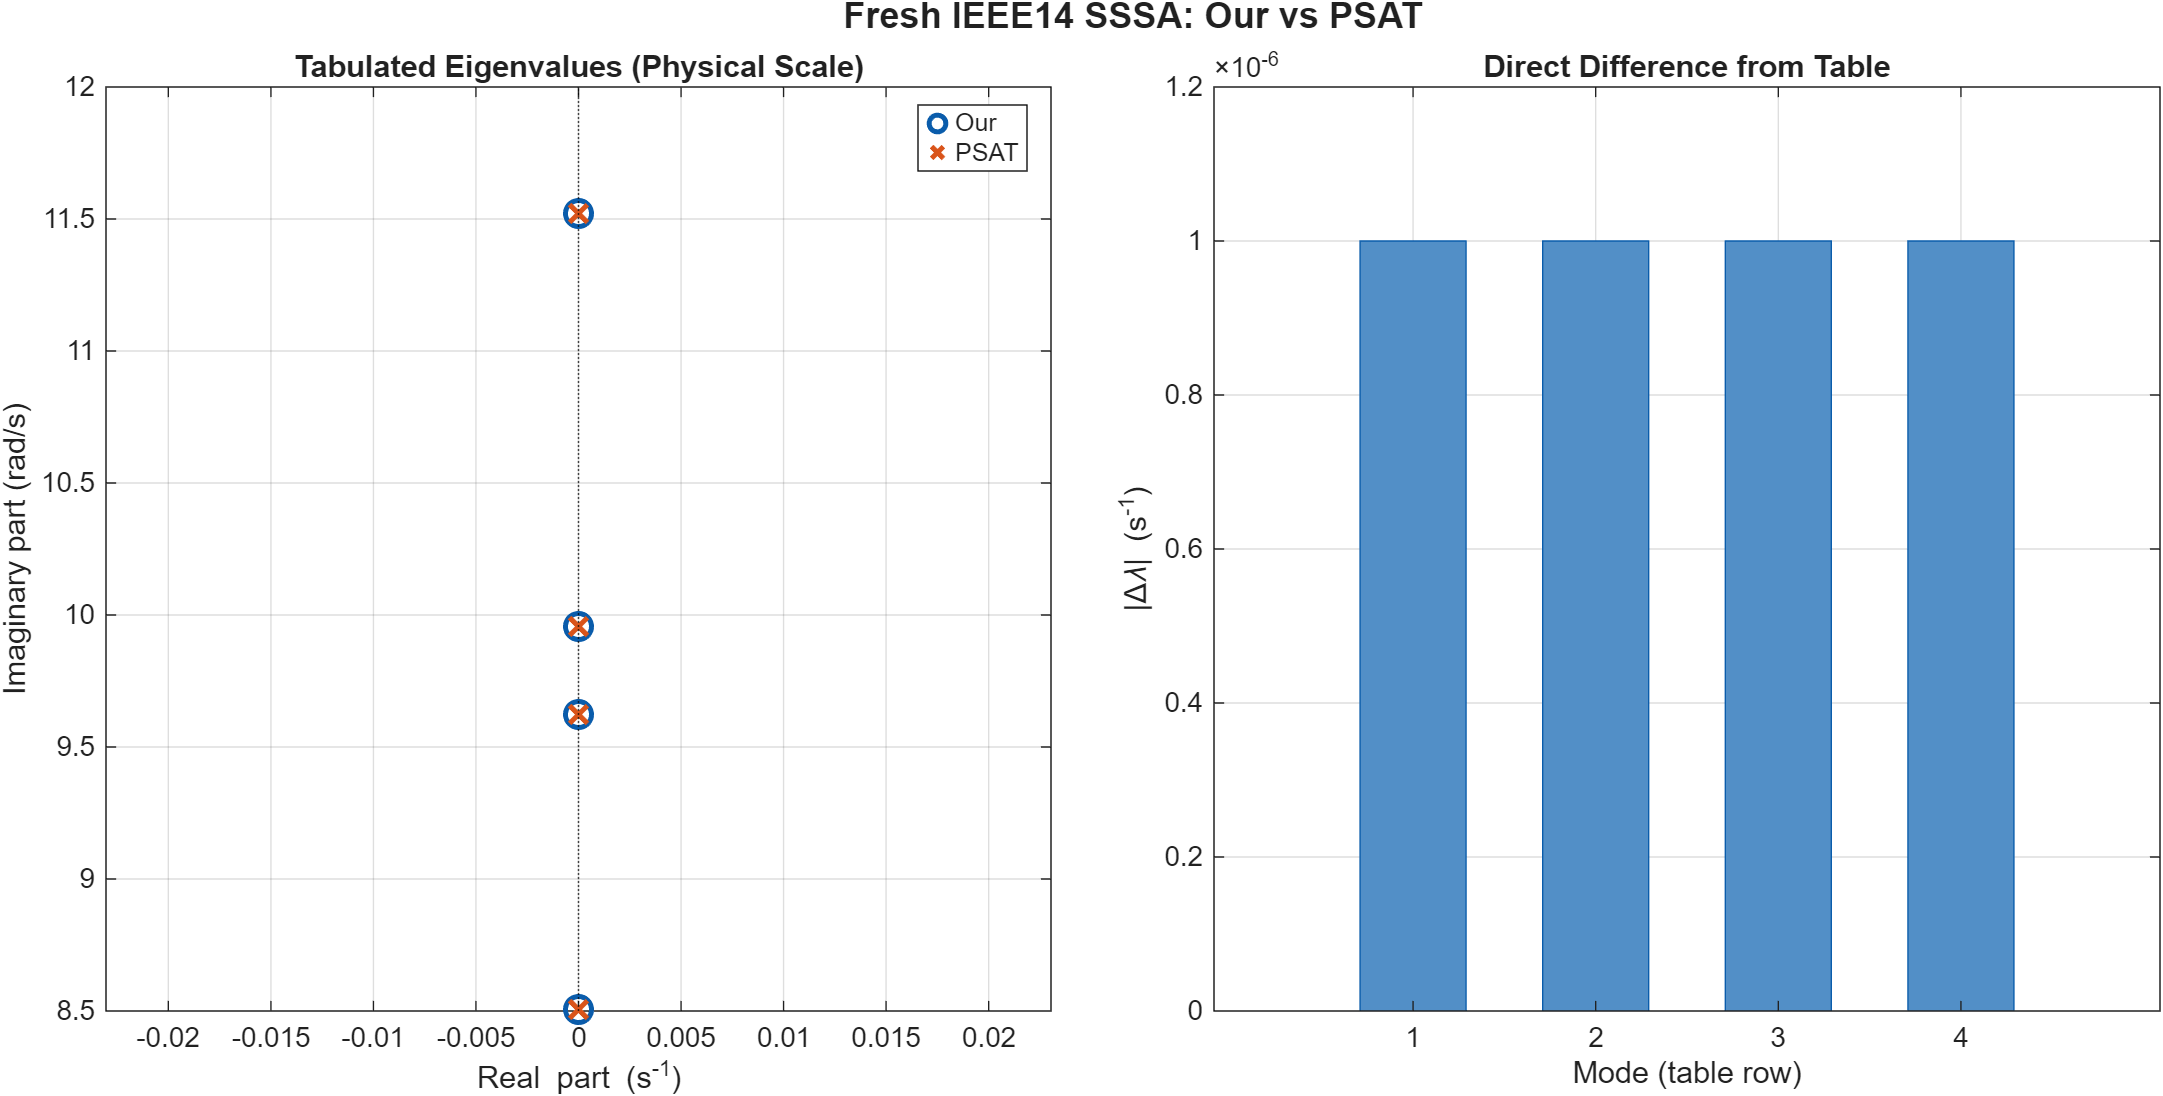
\includegraphics[width=.91\textwidth]{figures/padiyar_two_area/ieee14_sssa_complex_ours_psat.png}
\caption{Fresh IEEE14 positive-imaginary modes ที่ plot โดยตรงจาก Table~\ref{tab:ieee14-sssa} แผง complex-plane ใช้ unscaled eigenvalues ใน physical units; ส่วน difference panel รายงาน $|\Delta\lambda|$ ที่สอดคล้องสำหรับแต่ละ table row}
\label{fig:ieee14-sssa-complex}
\end{figure}

\begin{figure}[H]\centering
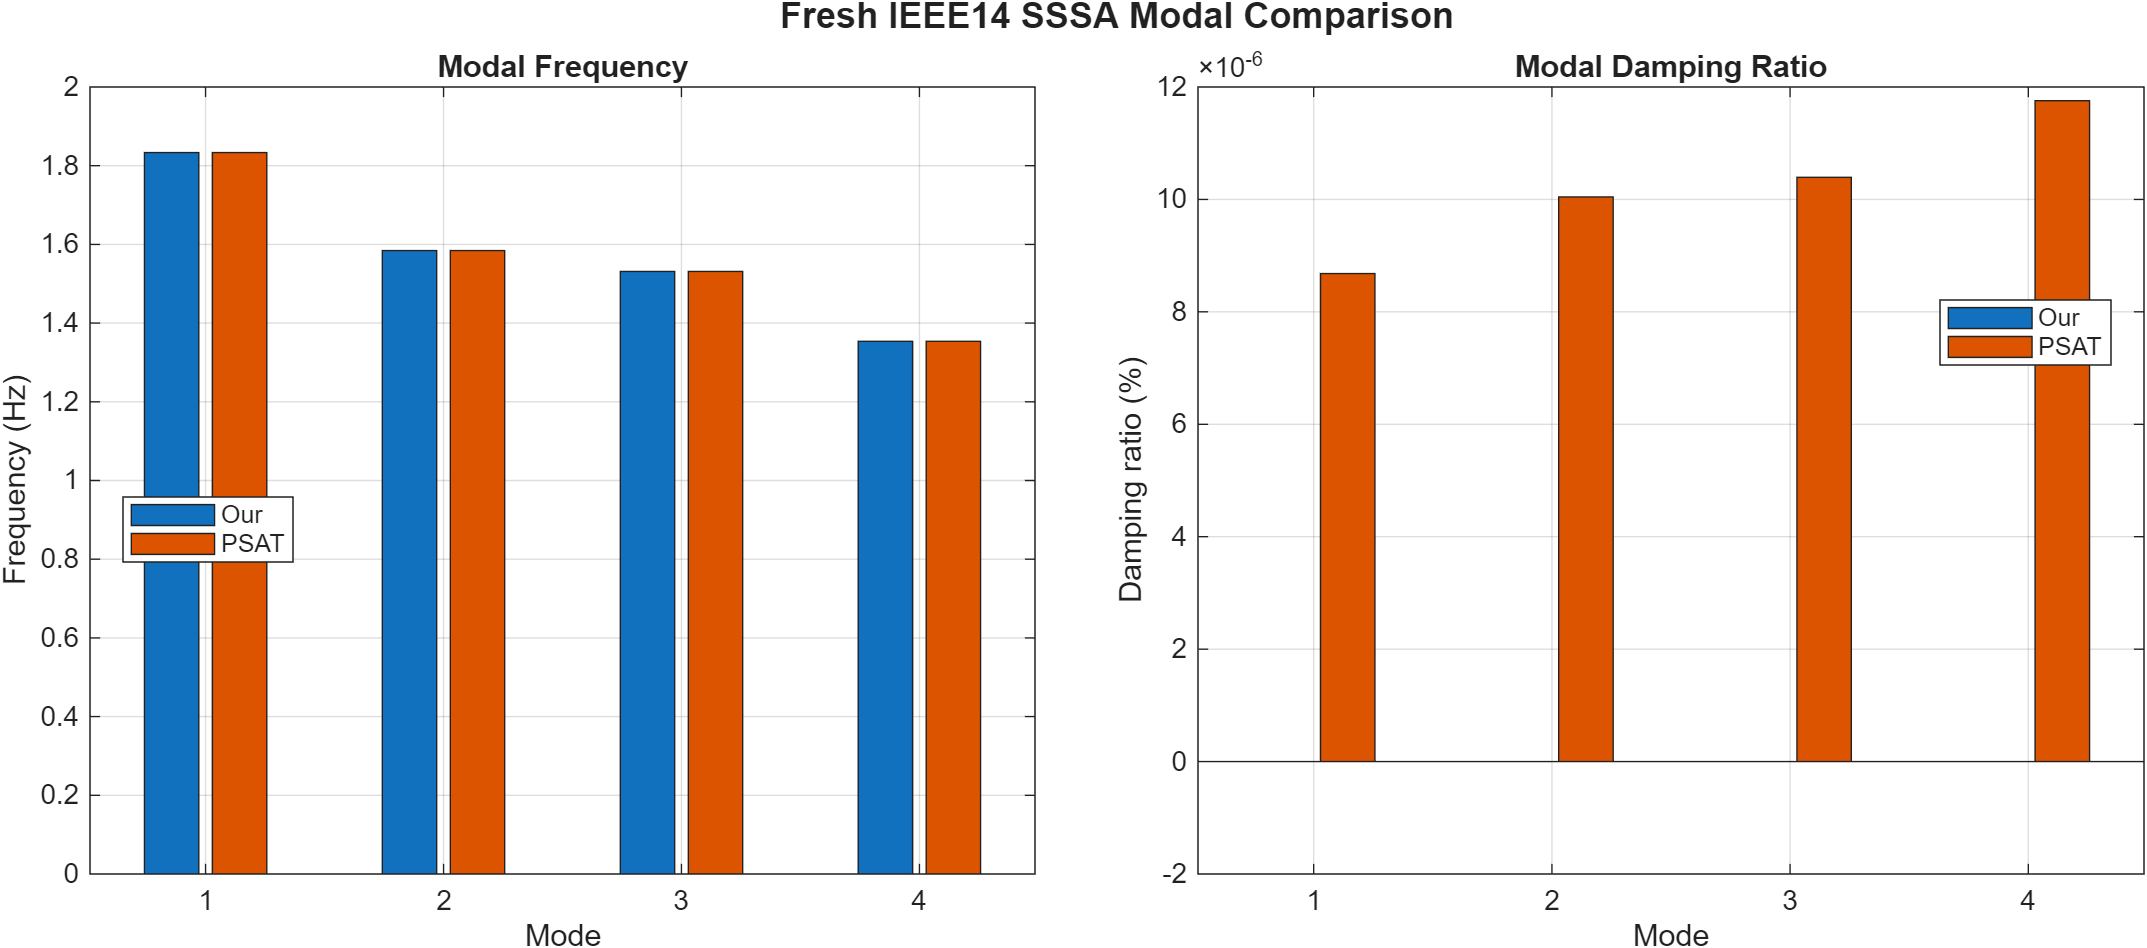
\includegraphics[width=.94\textwidth]{figures/padiyar_two_area/ieee14_sssa_modes_ours_psat.png}
\caption{Fresh IEEE14 modal frequencies และ damping ratios ที่สอดคล้องโดยตรงกับ Table~\ref{tab:ieee14-sssa}}
\label{fig:ieee14-sssa-modes}
\end{figure}

\subsection{Time-Domain Simulation Results}

Generator columns ถูก map โดย bus ID และ direct trajectory differences ถูกประเมินบน in-house event grid ส่วน in-house run เป็นไปตาม \path{solve_case('analysis','ts')} execution path และ MATPOWER14 defaults เดียวกันที่ใช้โดย \path{run_ts.m} ส่วน PSAT's additional internal event samples ถูก retain ใน raw count ของมัน; interpolation ไปยัง comparison grid จะ refuse extrapolation Table~\ref{tab:ieee14-ts} รายงานแต่ละ tool's response summary และ direct PSAT--Our differences ทั้งสี่ figures plot stored solver outputs: $\delta_i(t)$, $\omega_i(t)$, $P_{e,i}(t)$ และ bus-voltage magnitude ไม่มี COI, reference-machine, initial-angle หรือ speed-deviation transform ถูกใช้ ในทุก figure แผงบน overlay Our เป็น continuous lines และ PSAT เป็น cross markers ที่ sample จาก comparison grid เดียวกัน ทำให้ coincident trajectories มองเห็นได้ ส่วนแผงล่าง plot direct PSAT--Our difference

\begin{table}[H]\centering\small
\caption{Fresh IEEE14 TDS comparison สำหรับ bus-4, $Z_f=j10^{-4}$~pu fault}
\label{tab:ieee14-ts}
\resizebox{\textwidth}{!}{% Fresh Our and PSAT TS results on the declared scenario.
\begin{tabular}{llrr}\toprule
Metric & Unit & Our & PSAT \\ \midrule
Completed to 15 s & -- & Yes & Yes \\
Raw time points & points & 1501 & 1509 \\
Non-converged steps & steps & 0 & {Not exposed} \\
Minimum fault-bus voltage & pu & 0.000973 & 0.000973 \\
Maximum stored rotor-angle magnitude & deg & 4964.684009 & 4964.511399 \\
Maximum stored rotor-speed magnitude & pu & 1.040163906 & 1.040155053 \\
Maximum absolute electrical power & MW & 300.383981 & 300.376323 \\ \midrule
Maximum PSAT--Our rotor-angle difference & deg & {Reference} & 1.863392e-01 \\
Maximum PSAT--Our rotor-speed difference & pu & {Reference} & 9.867292e-06 \\
Maximum PSAT--Our electrical-power difference & MW & {Reference} & 1.225034e-01 \\
Maximum PSAT--Our bus-4 voltage difference & pu & {Reference} & 7.810489e-05 \\
\bottomrule\end{tabular}
}
\end{table}

\begin{figure}[H]\centering
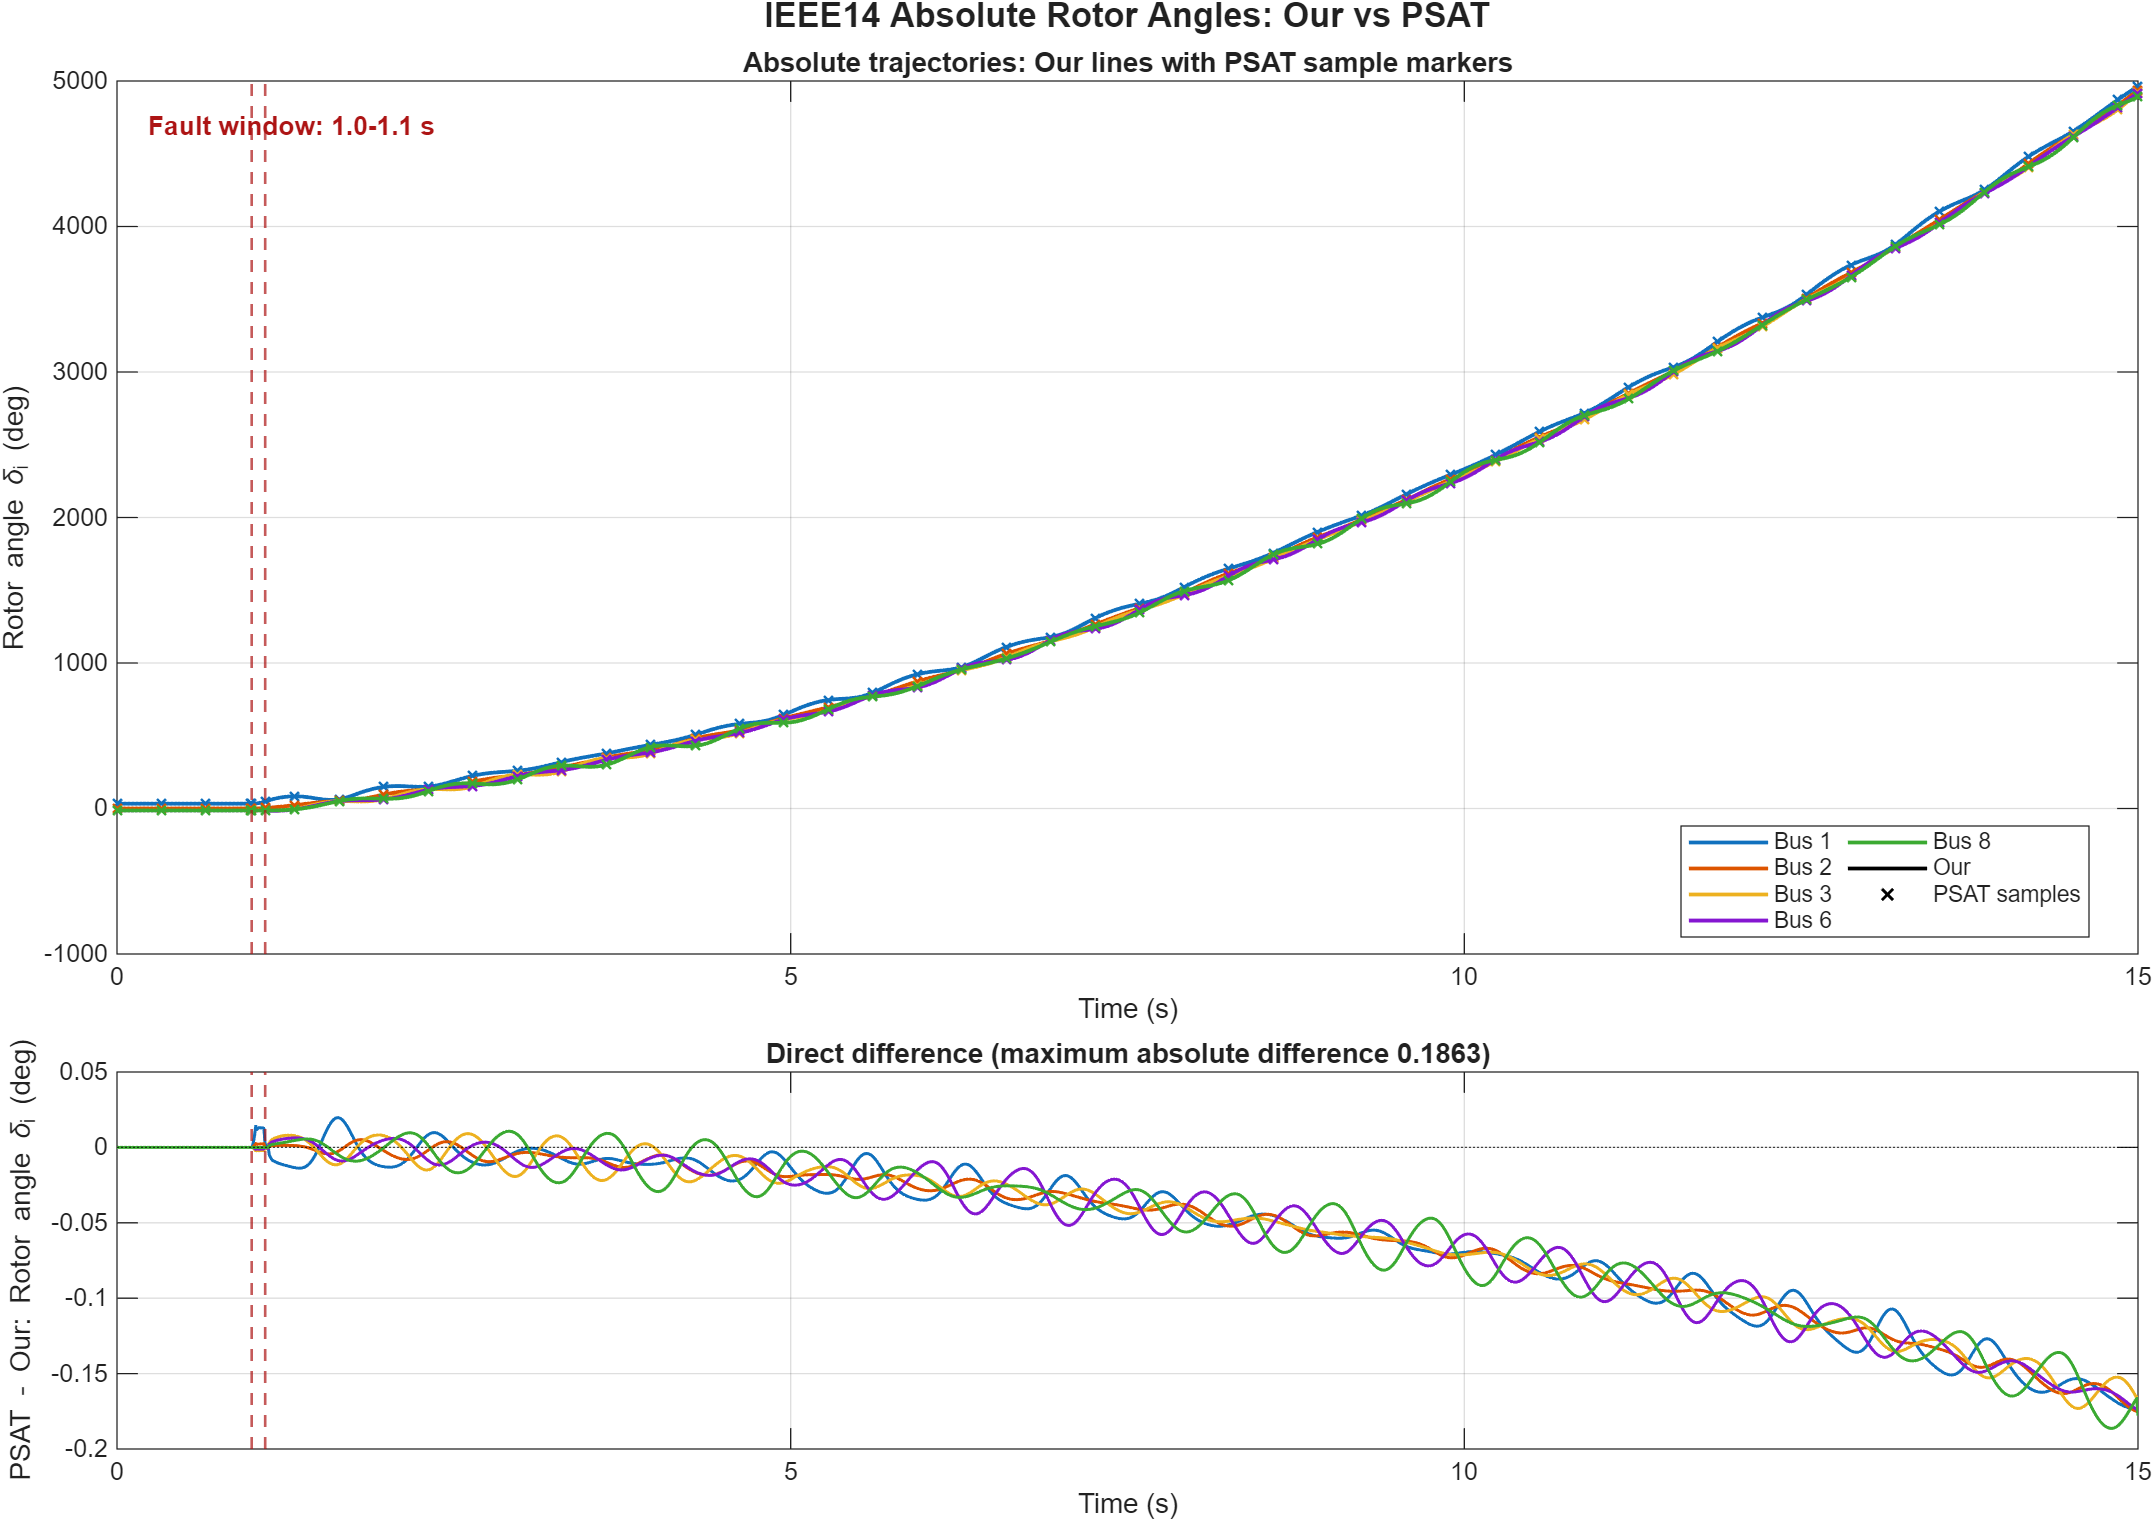
\includegraphics[width=.92\textwidth]{figures/padiyar_two_area/ieee14_ts_angle_ours_psat.png}
\caption{Fresh IEEE14 stored absolute rotor angles $\delta_i(t)$ สำหรับ 5 generator buses โดยใช้ \texttt{run\_ts.m} plotting convention ไม่มีการใช้ COI, reference-machine หรือ initial-angle subtraction สีระบุ buses แผงบน: Our lines และ PSAT cross markers แผงล่าง: direct PSAT--Our angle differences}
\label{fig:ieee14-ts-angle}
\end{figure}

\begin{figure}[H]\centering
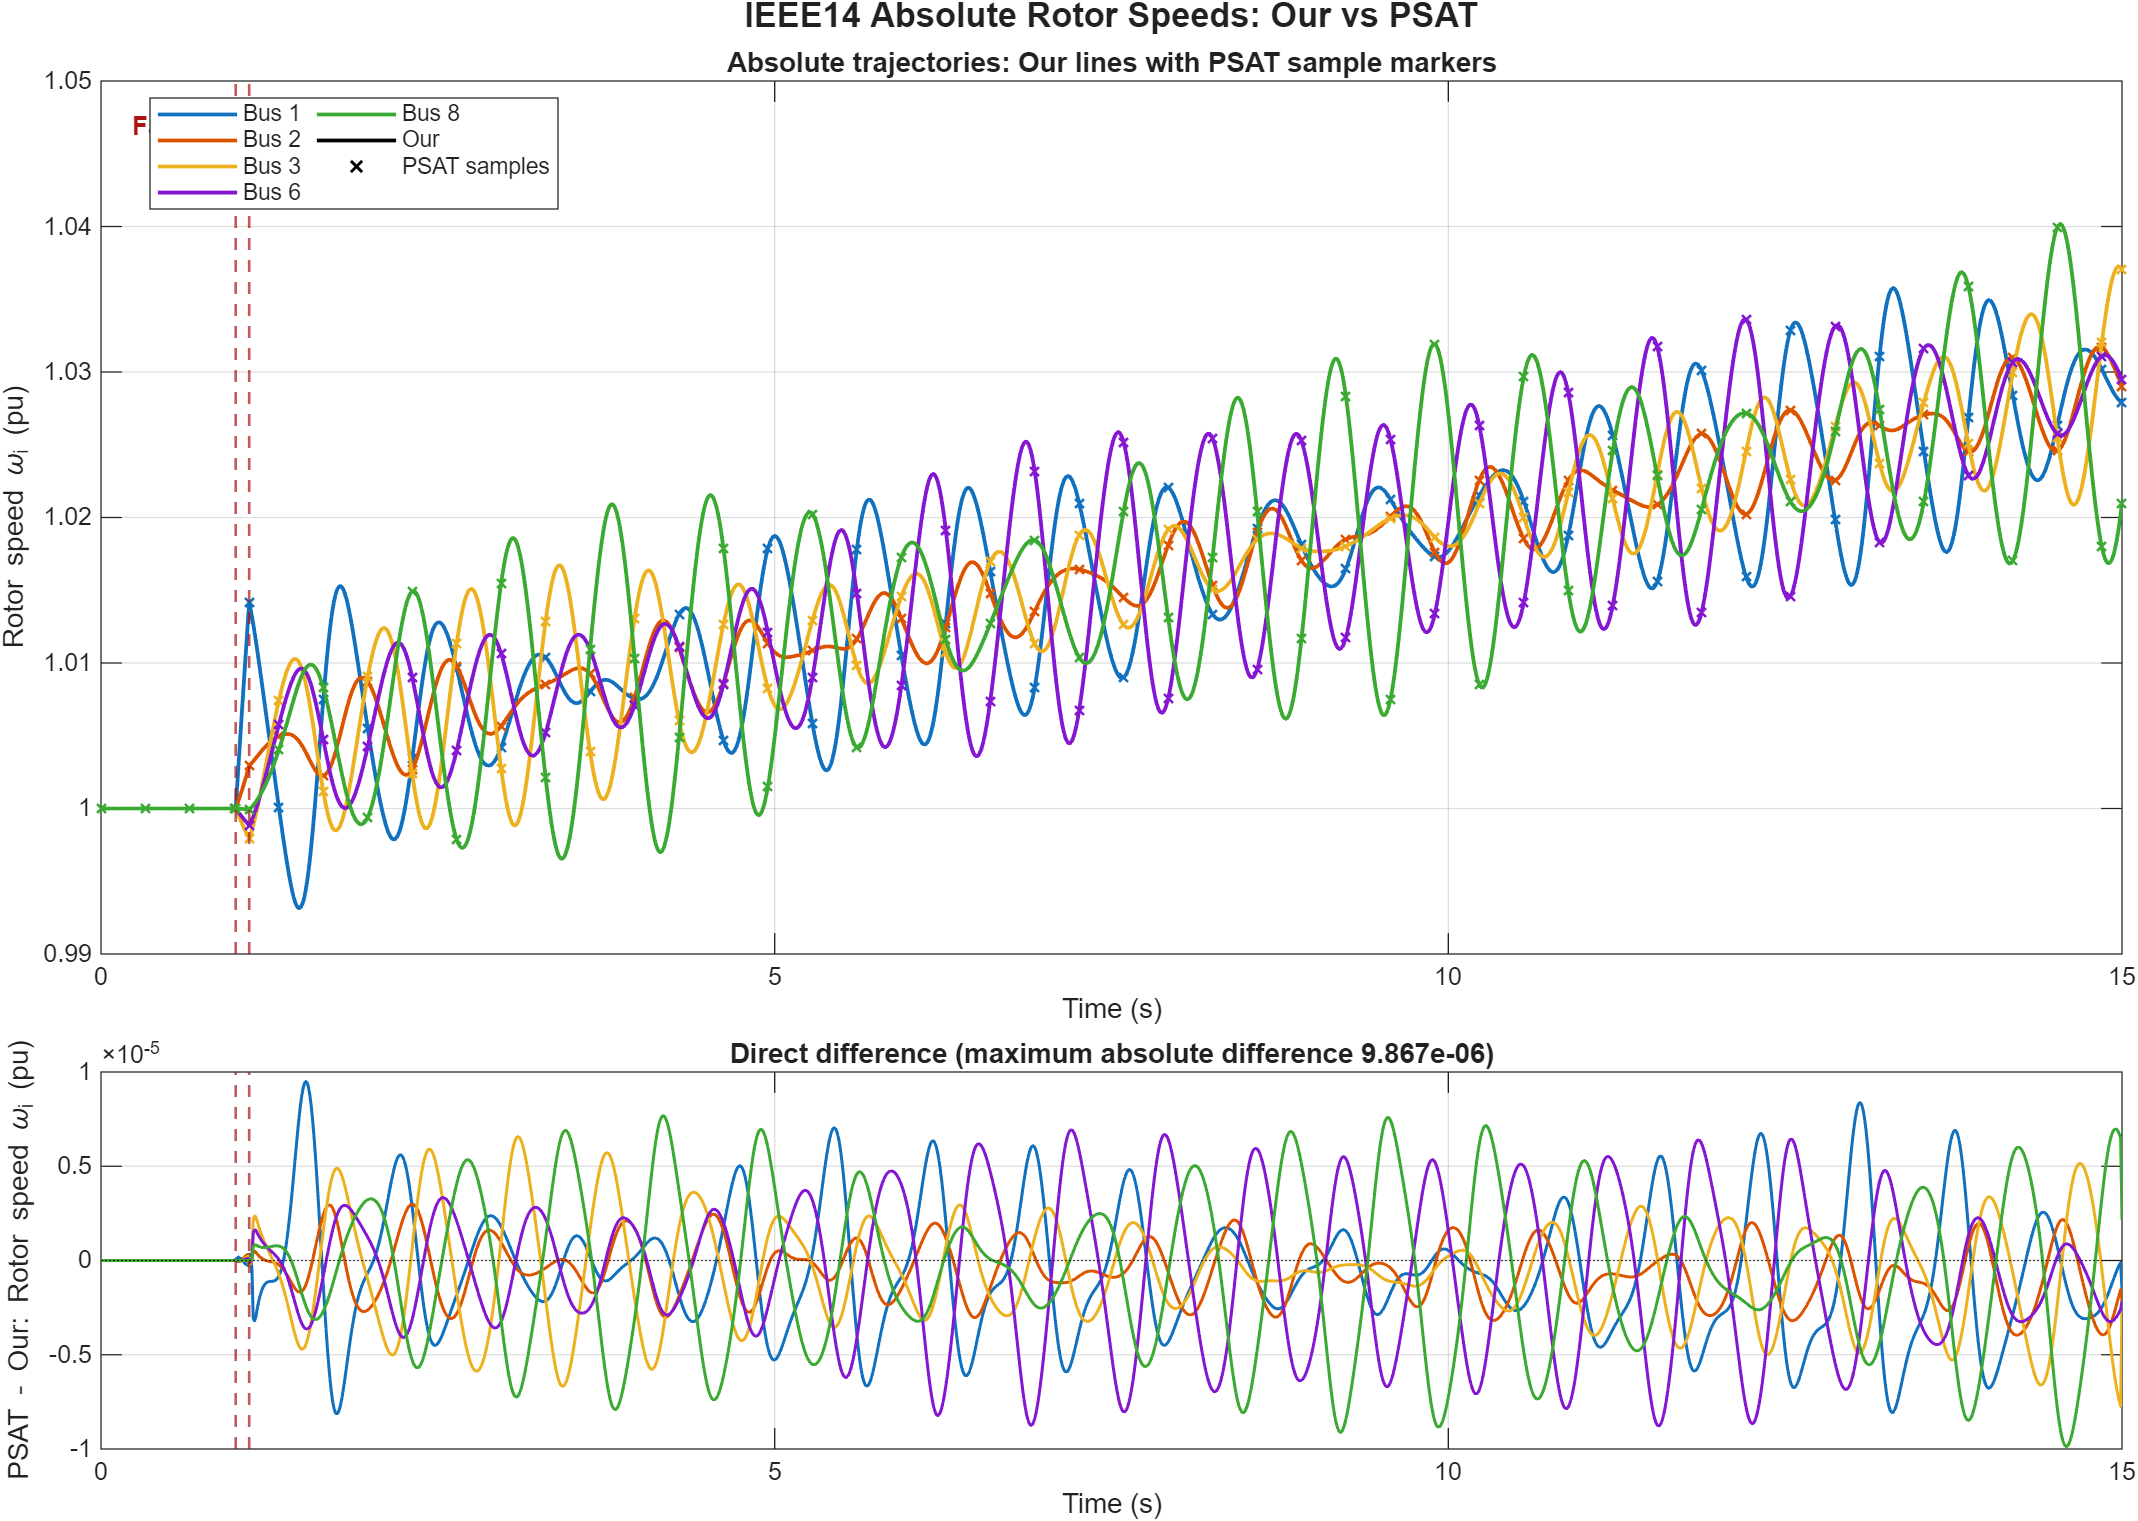
\includegraphics[width=.92\textwidth]{figures/padiyar_two_area/ieee14_ts_omega_ours_psat.png}
\caption{Fresh IEEE14 stored absolute rotor speeds $\omega_i(t)$ ใน per unit โดยใช้ \texttt{run\_ts.m} plotting convention ไม่มีการใช้ COI subtraction และไม่มีการใช้ $\omega_i-1$ transform แผงบน: Our lines และ PSAT cross markers แผงล่าง: direct PSAT--Our speed differences}
\label{fig:ieee14-ts-omega}
\end{figure}

\begin{figure}[H]\centering
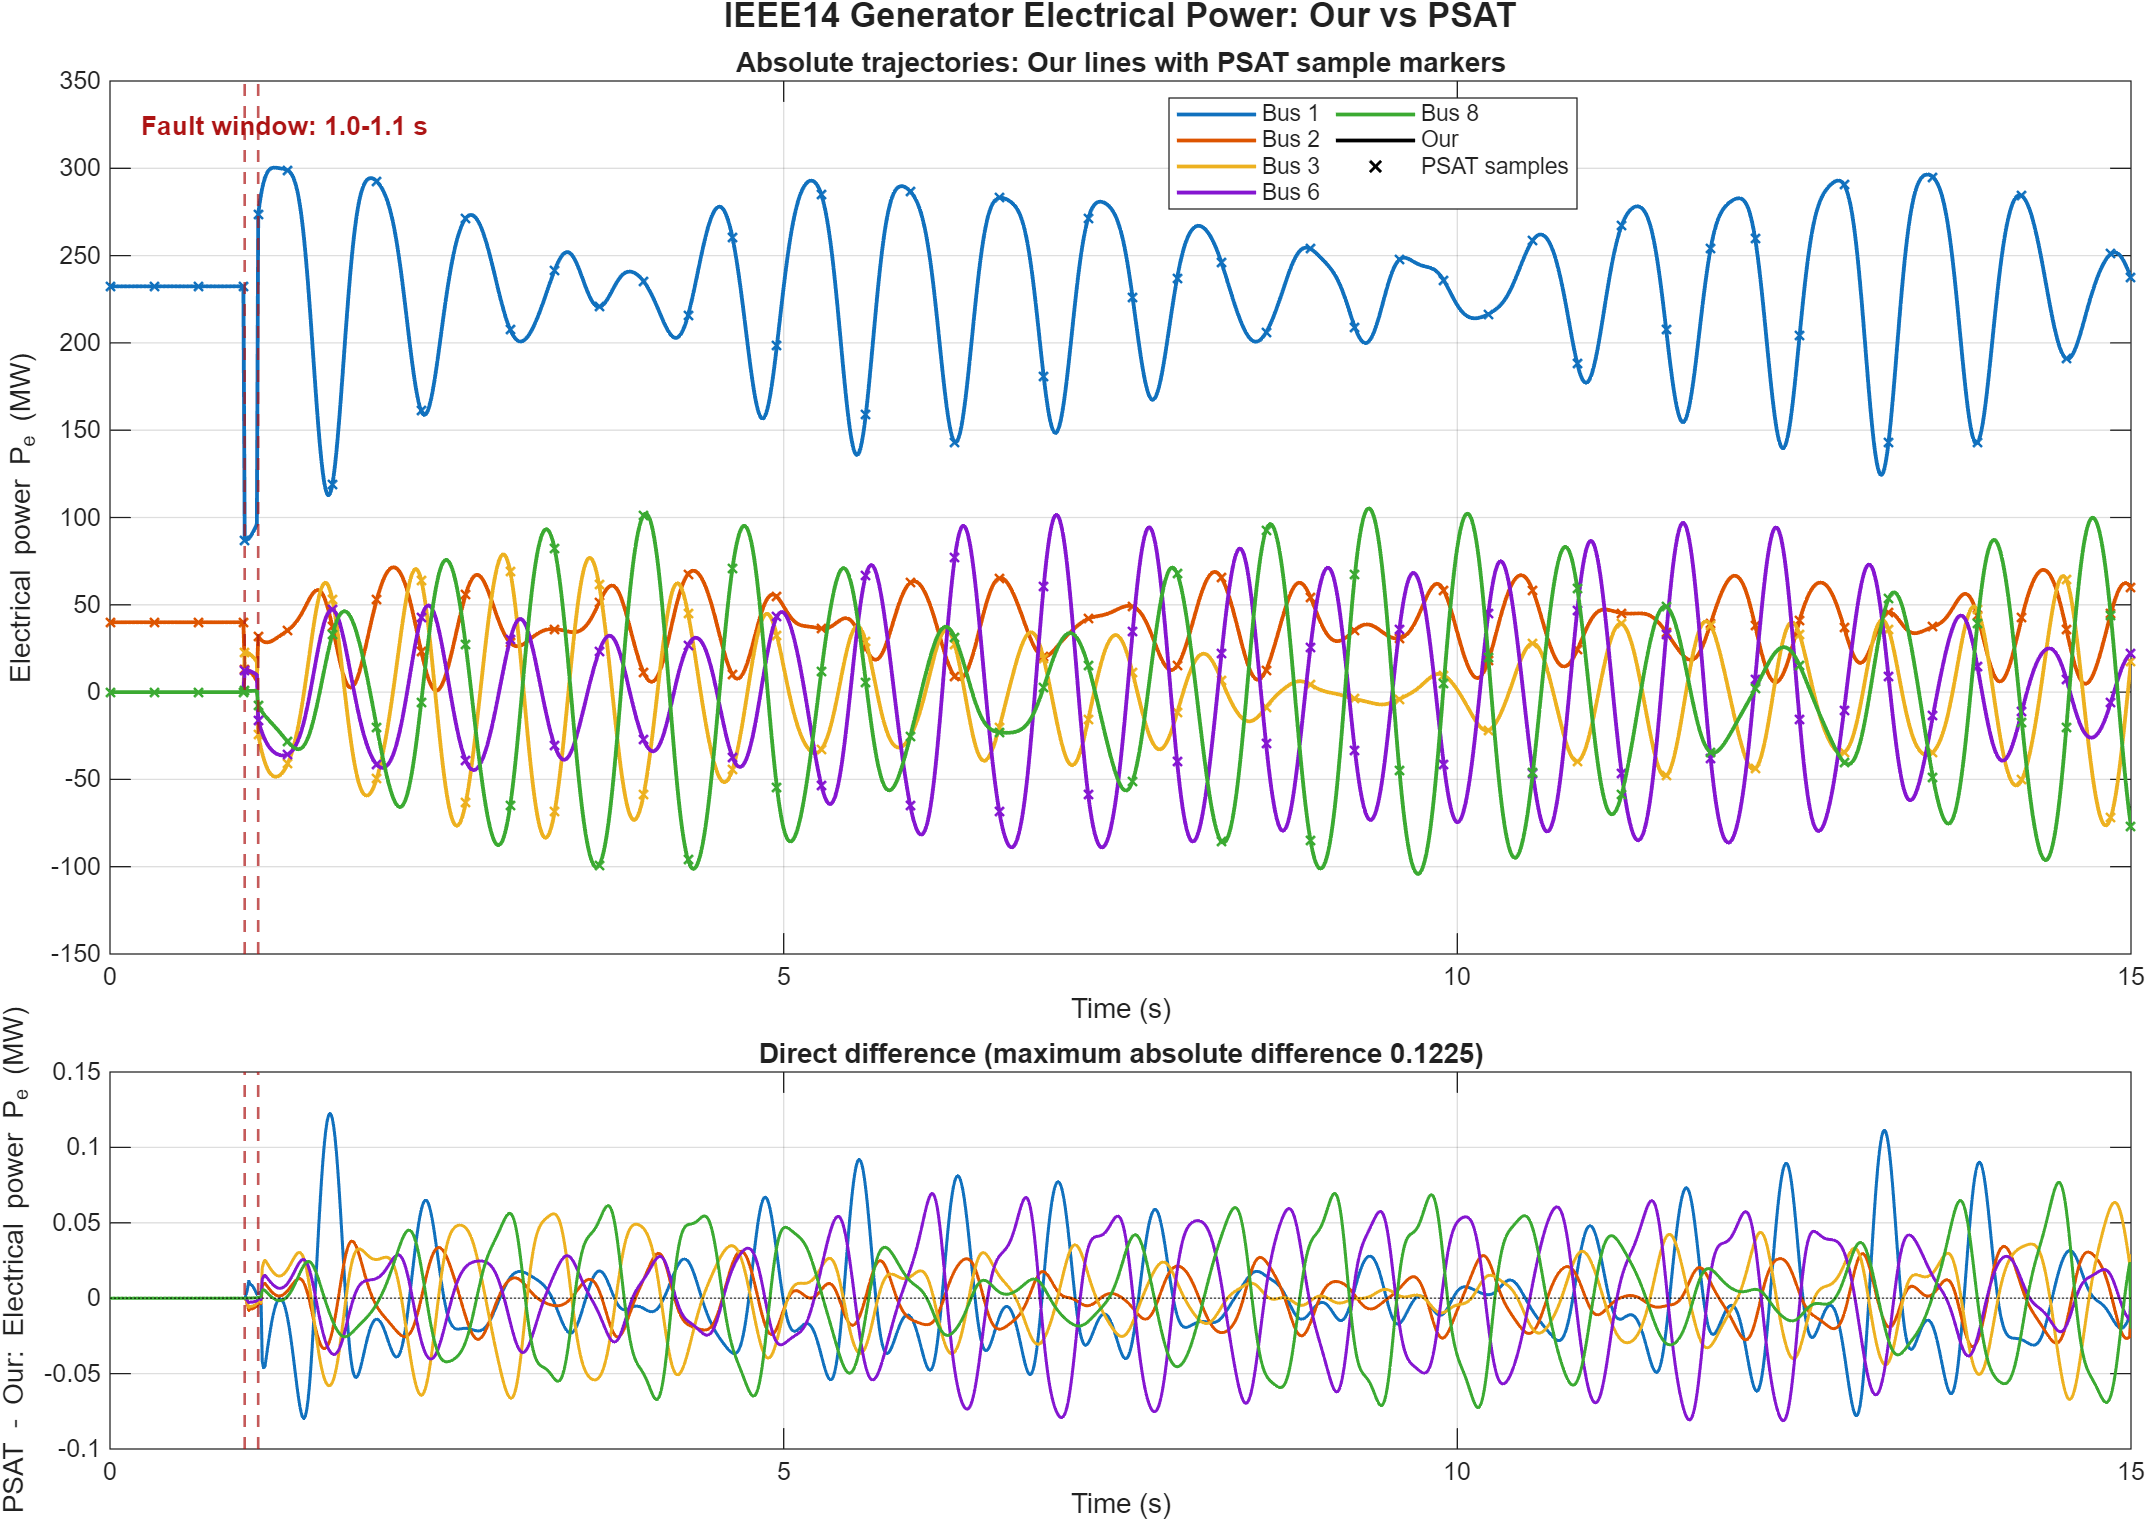
\includegraphics[width=.92\textwidth]{figures/padiyar_two_area/ieee14_ts_pe_ours_psat.png}
\caption{Fresh IEEE14 stored generator electrical powers $P_{e,i}(t)$ โดยใช้ \texttt{run\_ts.m} plotting convention แผงบน: Our lines และ PSAT cross markers แผงล่าง: direct PSAT--Our electrical-power differences}
\label{fig:ieee14-ts-pe}
\end{figure}

\begin{figure}[H]\centering
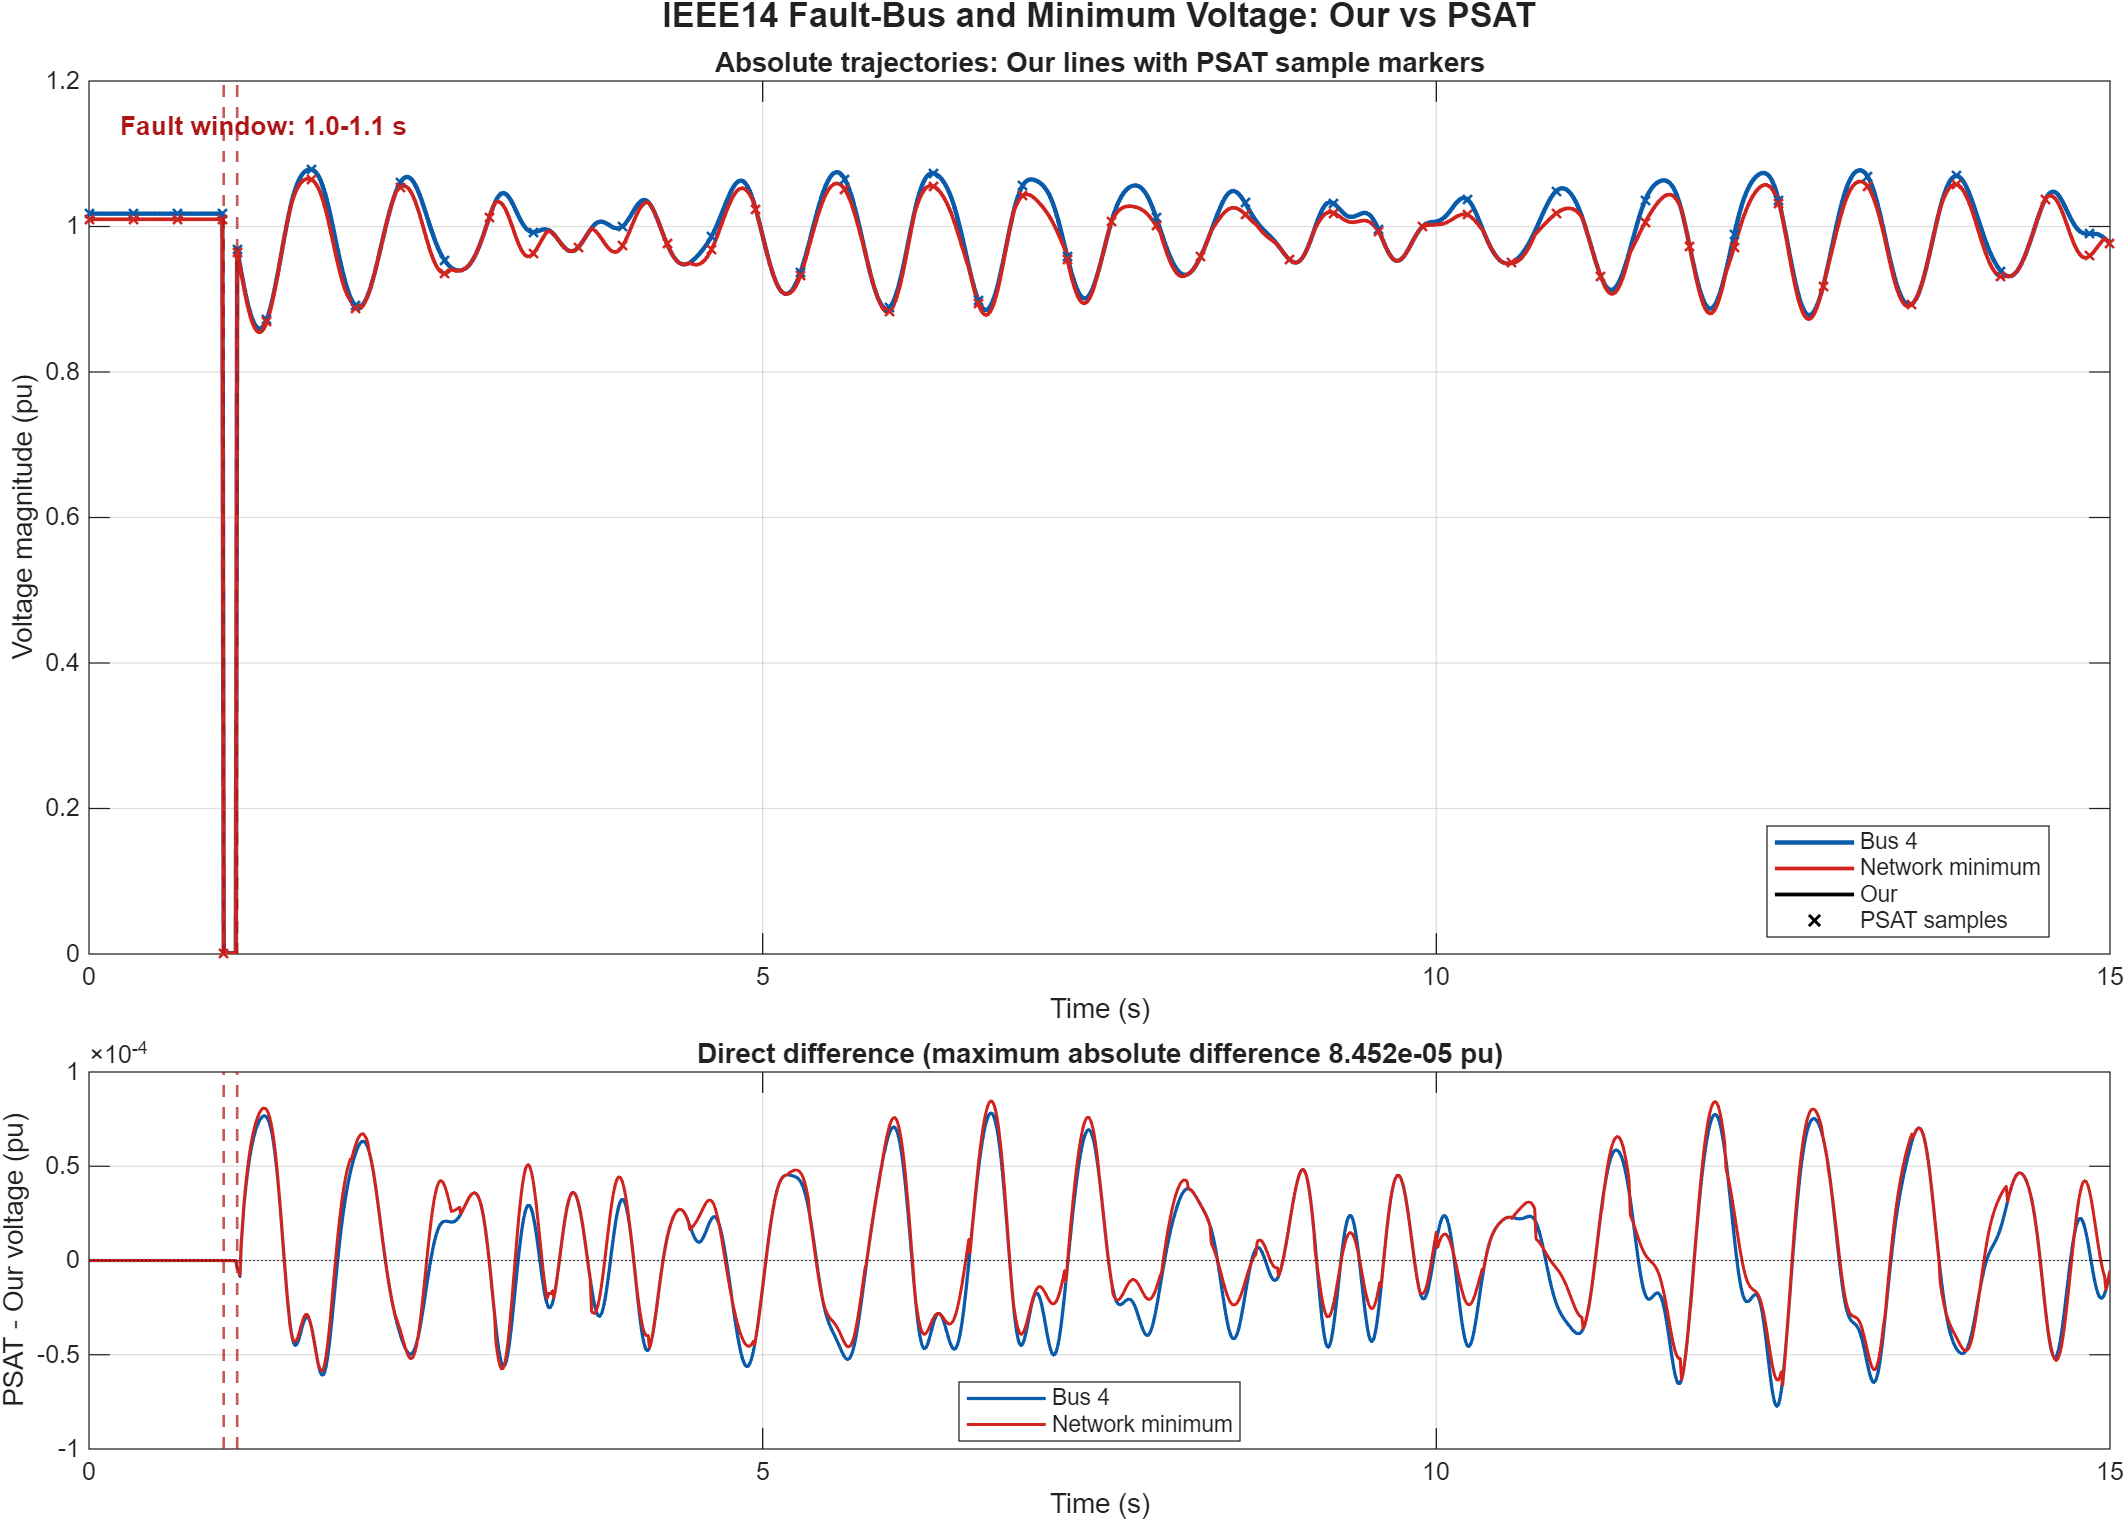
\includegraphics[width=.92\textwidth]{figures/padiyar_two_area/ieee14_ts_voltage_ours_psat.png}
\caption{Fresh IEEE14 bus-4 และ minimum-network voltage magnitudes สำหรับ declared fault โดยใช้ \texttt{run\_ts.m} plotting convention แผงบน: Our lines และ PSAT cross markers แผงล่าง: direct PSAT--Our voltage differences}
\label{fig:ieee14-ts-voltage}
\end{figure}

\section{สรุปผล (Conclusions)}

Padiyar two-area case ให้ traceable replacement reference สำหรับ project โดย reproduce Table~9.2 ด้วย in-house power flow, implement source's actual five-state AVR model, เปิดเผย manual-excitation comparison และรัน SSSA และ residual-checked TS จากหนึ่ง DAE ไม่มีการ fabricate subtransient parameter หรือ PSS setting ส่วนต่อขยายถัดไปอาจเพิ่ม documented PSS design และใช้ frozen SG baseline นี้สำหรับ SG-to-VSG replacement studies

\end{document}
